\documentclass[11pt]{article}
\usepackage[T1]{fontenc}
\usepackage[margin=1in]{geometry}
\usepackage{amsmath,amssymb,booktabs,hyperref}
% Adapted from Paper-code/SkiRentalForAdaptivity/camready/main.tex and plots/.
% Names are scoped so these snippets can also be included in the original paper.
\usepackage{pgfplots,booktabs,graphicx}
\usepgfplotslibrary{groupplots}
\usetikzlibrary{plotmarks}
\pgfplotsset{compat=1.18,
  skiqf axis/.style={
    label style={font=\small,align=center},
    tick label style={font=\scriptsize},
    title style={font=\small,align=center},
    legend style={font=\small,draw=none},
    grid=major,grid style={line width=.2pt,draw=gray!50},
    scaled ticks=false,
  },
  skiqfNonAdaptive/.style={color=gray,mark=pentagon*,mark options={color=gray}},
  skiqfAdaptive/.style={color=cyan,mark=square*,mark options={color=cyan}},
  skiqfSki/.style={color=magenta,mark=halfcircle*,mark options={color=magenta}},
  skiqfRandomized/.style={color=orange,mark=star,mark options={color=orange}},
  skiqfHybrid/.style={color=blue,mark=halfsquare*,mark options={color=blue}},
  skiqfNonAdaptiveBar/.style={fill=lightgray,draw=lightgray},
  skiqfAdaptiveBar/.style={fill=cyan,draw=cyan},
  skiqfSkiBar/.style={fill=magenta,draw=magenta},
  skiqfRandomizedBar/.style={fill=orange,draw=orange},
  skiqfHybridBar/.style={fill=blue,draw=blue},
}

\title{Randomized Ski Rental and RandomizedSkiQF}
\author{Background and analysis}
\date{November 2026}
\begin{document}
\maketitle
\begin{abstract}
This report separates classical ski-rental theory from its application to RandomizedSkiQF. Part I explains the classical rental model, the randomized purchase rule, and its expected competitive guarantee. Part II develops workload-dependent cost comparisons relevant to RandomizedSkiQF, including uniform occurrence counts and query-frequency distributions. The latter calculations are consequences of the idealized rental model, not measurements or a competitive proof for the integrated filter.
\end{abstract}
\part{The classical randomized ski-rental algorithm}
\section{The decision problem}
You need skis on each day of a season, but do not know how many days the season will last. Renting costs $r$ per day. Buying costs $br$ once and covers that day and all later days. Divide all costs by $r$: renting now costs 1 and buying costs $b$. Buying replaces renting on the purchase day; it does not incur an additional day's rental charge.

Initially assume that $b=B$ is a positive integer. The season length $n\ge1$ is an integer revealed one day at a time. On day $k$, you know that day $k$ exists, but not whether day $k+1$ will exist. The price is fixed, purchase is always available, and ownership is permanent. These assumptions define the problem being analyzed.

An offline algorithm knows $n$ in advance. It either rents throughout or buys on the first day, so
\[
\mathrm{OPT}(n)=\min(n,B).
\]
An online algorithm has to decide without that knowledge. If it plans to buy on day $K$, its total cost is
\[
C(n,K)=\begin{cases}n,&n<K,\\K-1+B,&n\ge K.\end{cases}
\]
The purchase happens only if the season reaches day $K$.

\section{The deterministic baseline}
The standard deterministic rule rents for $B-1$ days and buys on day $B$. If $n<B$, it is optimal. If $n\ge B$, its cost is $2B-1$, compared with offline cost $B$. Its worst-case ratio is therefore
\[
\rho_{\mathrm{det}}=2-\frac1B.
\]
For integer $B$, this is optimal among deterministic algorithms. Buying earlier on day $k<B$ lets the adversary stop on day $k$, giving ratio $(k-1+B)/k=1+(B-1)/k\ge2-1/B$. Buying later gives a long-season cost greater than $2B-1$; never buying has unbounded ratio. Before purchasing, the only new information is that the season continues, so a deterministic policy is characterized by such a purchase day.

The vulnerability is uncertainty about the stopping time. A purchase just before the season ends wastes money, while waiting too long wastes rental payments. Randomization balances these risks across different season lengths.

\section{What ``competitive in expectation'' means}
For a randomized algorithm, $K$ is random. A ratio $\rho$ means
\[
\text{for every fixed }n\ge1,\qquad
\mathbb E_K[C(n,K)]\le\rho\,\mathrm{OPT}(n).
\]
Equivalently, the competitive ratio is $\sup_n\mathbb E_K[C(n,K)]/\mathrm{OPT}(n)$. The expectation is over the algorithm's private random choices. No probability distribution on season lengths is assumed.

This is the oblivious-adversary model: the adversary can know the purchase distribution but must choose the season independently of the realized random choices. An adversary that observes the purchase and immediately ends the season changes the problem. Also, the inequality is an expected-cost statement, not a guarantee for every run or a high-probability bound.

The classical optimal limiting ratio is $e/(e-1)\simeq1.582$, as recalled in the ski-rental literature~\cite{background}. The frequently quoted deterministic ratio 2 and randomized ratio 1.582 are limiting values; integer purchase costs admit the sharper finite-$B$ expressions below.

\section{The randomized purchase rule}
For $B\ge2$, define $q=1-1/B$ and sample
\[
\boxed{\Pr(K=k)=p_k=\frac{q^{B-k}}{B(1-q^B)},\qquad k=1,\ldots,B.}
\]
Then rent on days before $K$ and buy on day $K$, if it occurs. This is not a uniform random threshold: later days have larger probability, with $p_{k+1}=p_k/q$. The geometric-series identity gives
\[
\sum_{k=1}^B p_k=
\frac{1-q^B}{B(1-q)(1-q^B)}=1.
\]
For $B=1$, buy on the first day deterministically.

The algorithm makes one random choice per season, before observing its length:
\begin{enumerate}
\item Sample one purchase day $K$ from $p_1,\ldots,p_B$.
\item Rent on every day before $K$ that actually occurs.
\item If day $K$ occurs, buy then; otherwise the season ends without a purchase.
\end{enumerate}
Once $K$ has been sampled, all subsequent actions are deterministic. There is no further random decision during the season.

To sample this distribution concretely, draw one uniform number $U\in[0,1)$ and choose the smallest $c$ such that $U<\sum_{j=1}^{c}p_j$. The interval assigned to day $c$ has length $p_c$, so the probability of selecting that day is exactly $p_c$.

\section{Deriving the purchase-day distribution}
Karlin et al. describe a randomized algorithm as a probability distribution over deterministic threshold algorithms. They write the inequalities needed for a competitive guarantee, set them to equalities, solve the resulting difference equations, and normalize the probabilities~\cite{karlin}. The following gives that construction in ski-rental notation; the original paper uses a caching problem with different cost conventions.

Let $p_c$ be the probability of choosing the deterministic algorithm that buys on day $c$. For a season of length $n\le B$, its expected cost is
\[
E_n=\sum_{c=1}^n (B+c-1)p_c
+n\sum_{c=n+1}^B p_c.
\]
The first sum covers choices that buy before the season ends. The second covers choices that rent throughout. For $n\ge B$, every choice has bought, so $E_n=E_B$.

Our objective is to choose nonnegative probabilities summing to one and the smallest possible $\rho$ such that
\[
\begin{cases}
E_n\le\rho n,&1\le n\le B,\\
E_n\le\rho B,&n>B.
\end{cases}
\]
These are simply the competitive-ratio requirements, since the offline cost is $\min(n,B)$. Together with $p_c\ge0$ and $\sum_c p_c=1$, minimizing $\rho$ is a linear program: each expected cost $E_n$ is a linear function of the probabilities. Only the first $B$ cost constraints are needed because costs stop changing after day $B$.

Geometrically, we lower $\rho$ until lowering it further would make the constraints infeasible. An optimum can be chosen at a vertex of the feasible polyhedron, where some constraints are tight. Linear programming alone does not imply that every cost constraint is tight. For this ski-rental construction, setting all $B$ cost constraints to equality produces the classical candidate distribution.

Following Karlin's construction, set these inequalities to equalities and solve for the probabilities. For the first $B$ horizons, this means
\[
E_1=\rho,\quad E_2=2\rho,\quad\ldots,\quad E_B=B\rho.
\]
This step looks for a distribution that balances the expected ratio across season lengths. It is a way to construct the algorithm, not an extra assumption about the input or the definition of competitiveness. After solving, we verify that the probabilities are valid and that they satisfy the required bound. Proving that no other algorithm does better is a separate lower-bound argument.

\paragraph{Step 1: Express the cost of one more day.}
Couple seasons of length $c-1$ and $c$ by using the same planned purchase day $K$. If $K<c$, both seasons have already paid for skis and the cost increment is zero. If $K=c$, the longer season buys for $B$, whereas the shorter season stops after renting for $c-1$ days. If $K>c$, the longer season pays one more rental. Therefore
\begin{equation}
E_c-E_{c-1}=Bp_c+\sum_{k=c+1}^B p_k.
\label{eq:increment}
\end{equation}
Since we set $E_c=\rho c$ and $E_{c-1}=\rho(c-1)$, subtracting gives $E_c-E_{c-1}=\rho$. For $c=1$, use $E_0=0$.

\paragraph{Step 2: Eliminate the unknown ratio.}
For consecutive days $c$ and $c+1$, with $c<B$, we require
\begin{align*}
Bp_c+p_{c+1}+\sum_{k=c+2}^B p_k&=\rho,\\
Bp_{c+1}+\sum_{k=c+2}^B p_k&=\rho.
\end{align*}
Subtracting the second equation from the first gives
\[
Bp_c-(B-1)p_{c+1}=0,
\qquad p_c=\left(1-\frac1B\right)p_{c+1}=q p_{c+1}.
\]
Iterating backward from the last day yields $p_c=q^{B-c}p_B$.

\paragraph{Step 3: Normalize the distribution.}
Since the policy buys on one of days $1,\ldots,B$,
\[
1=\sum_{c=1}^B p_c
=p_B\sum_{j=0}^{B-1}q^j
=p_B\frac{1-q^B}{1-q}.
\]
Thus $p_B=(1-q)/(1-q^B)$, and substitution gives
\[
\boxed{p_c=\frac{(1-q)q^{B-c}}{1-q^B}
=\frac{q^{B-c}}{B(1-q^B)}.}
\]
All terms are positive for $B>1$, so this is a valid probability distribution. On day $B$, equation~\eqref{eq:increment} gives $\rho=Bp_B=1/(1-q^B)$. The recurrence ensures every earlier increment has that same value. Thus the equations produce a valid distribution with the desired expected costs.

\section{Deriving the expected guarantee}
The recurrence and normalization above give
\[
E_c-E_{c-1}=\rho_B,\qquad
\rho_B=\frac1{1-(1-1/B)^B},\quad 1\le c\le B.
\]
Starting from $E_0=0$ and summing these increments gives $E_n=\rho_B n$ for $n\le B$. For $n>B$, every possible sampled purchase day has already occurred, so $E_n=E_B=\rho_BB$. Combining the two cases,
\[
\boxed{\mathbb E_K[C(n,K)]=\rho_B\min(n,B)
=\rho_B\mathrm{OPT}(n).}
\]
This proves the expected guarantee for every fixed season length. The separate assertion that no randomized policy can achieve a smaller worst-case ratio requires a minimax lower-bound proof, which is not reproduced here.

Since $(1-1/B)^B\to e^{-1}$,
\[
\rho_B\longrightarrow\frac{e}{e-1}=1.5819767\ldots.
\]
For finite integer $B>1$, $\rho_B$ is smaller than this limit and smaller than $2-1/B$.
\begin{center}
\begin{tabular}{rrr}
\toprule
Purchase cost $B$&Randomized ratio&Deterministic ratio\\
\midrule
1&1.0000&1.0000\\
2&1.3333&1.5000\\
3&1.4211&1.6667\\
5&1.4874&1.8000\\
10&1.5353&1.9000\\
$B\to\infty$&1.5820&2.0000\\
\bottomrule
\end{tabular}
\end{center}

\section{A better worst-case guarantee does not mean lower cost on every season}
For $n<B$, deterministic ski rental pays $n$, whereas the randomized rule pays $\rho_Bn$ in expectation. Randomization pays a premium on short seasons. For $n\ge B$, it saves
\[
\Delta_B=2B-1-\rho_BB
\]
relative to the deterministic rule. It trades some short-season performance for better protection when the season is long.

If a separate application model supplies a random horizon $N$, independent of the algorithm's coins, the randomized rule has lower average modeled cost precisely when
\[
\Pr(N\ge B)\Delta_B>
(\rho_B-1)\mathbb E[N\mathbf1_{\{N<B\}}].
\]
This is an algebraic comparison of the two cost functions, not an assumption needed by competitive analysis.

\clearpage
\part{Workload implications for RandomizedSkiQF}
\section{The application model and its scope}
The following calculations apply the classical cost functions to idealized independent adaptation instances. Let a missed opportunity to adapt incur a false-positive database lookup of cost $R$, and let adaptation add cost $A$. Under the convention that the triggering lookup must also be paid, the normalized purchase cost is $B=1+A/R$. We assume this is an integer and that both policies use this calibrated cost. An instance with $N$ occurrences would incur $N$ false positives if it were never corrected; a successful purchase eliminates the remaining ones.

For general $\alpha=A/R$, with deterministic threshold $t$, the total cost is $k$ when $k<t$ and $t+\alpha$ otherwise. For a sampled threshold with probabilities $p_c$,
\[
E[C(k,K)]=k\Pr(K>k)+\sum_{c=1}^{\min(k,B)}p_c(c+\alpha).
\]
The classical simplification $\rho_B\min(k,B)$ requires integer $B=1+\alpha$. For any other supplied threshold and cost ratio, use the full expression rather than claiming that same calibrated guarantee.

These assumptions let us compare policies mathematically before measuring the system. They do not identify every query key with an independent instance in the actual filter: fingerprints can share state, and one adaptation can affect several keys. Space limits, failed adaptations, CPU work, and changing access costs also fall outside the formulas. No implementation changes are made or assumed here.

\section{Known workload distributions change the optimization objective}
Competitive analysis minimizes a worst-case ratio over horizons. If instead the horizon $N$ follows a known distribution, an average-cost objective is
\[
\min_{\text{policy}}\ \mathbb E_{N,K}[C(N,K)].
\]
These objectives can prefer different policies. In particular, the classical randomized rule is not designed to minimize expected cost for every distribution of $N$.

For a fixed purchase threshold $k$, define
\[
L(k)=\mathbb E_N[C(N,k)]
=\sum_{n=0}^{k-1}n\Pr(N=n)+(k-1+B)\Pr(N\ge k).
\]
Allow $k=\infty$ to mean never buy, with $L(\infty)=\mathbb E[N]$. A randomized threshold, sampled independently of $N$ with probabilities $a_k$, has average cost
\[
\mathbb E_{N,K}[C(N,K)]=\sum_k a_kL(k)\ge\inf_k L(k).
\]
For finite workloads the minimum is attained, so a best deterministic threshold achieves at least as low an average cost as any mixture. This is a linear objective over a probability simplex: select a threshold with smallest coefficient $L(k)$. It does not say that the standard deterministic threshold $k=B$ is best for every known workload distribution. Nor does it address policies that observe additional predictive information beyond the occurrence count.

\section{Which occurrence distributions favor randomization?}
For comparison with deterministic purchase at $B$, define
\[
\Delta_B=2B-1-\rho_BB.
\]
For $B>1$, this is positive. On each instance shorter than $B$, the randomized policy pays an expected premium $(\rho_B-1)N$. On each instance reaching $B$, it saves $\Delta_B$. Averaging gives
\begin{equation}
\mathbb E[C_{\mathrm{rand}}-C_{\mathrm{det}}]
=(\rho_B-1)\mathbb E[N\mathbf1_{\{N<B\}}]
-\Delta_B\Pr(N\ge B).
\label{eq:workload-difference}
\end{equation}
Thus the sign depends on both the probability of long instances and the total expected rental cost of short instances. If every instance has $N<B$, deterministic rental is offline-optimal on each one. If every instance has $N\ge B$, randomization has strictly smaller expected cost for $B>1$. A distribution being ``random'' by itself implies neither conclusion.

\subsection{The selected once-or-twice experiment}
Let $f$ denote the fraction of distinct absent query keys occurring once. Every other key occurs twice. At nominal $\alpha=1$, $B=2$, the predicted costs per initially false-positive instance are
\[
E[C_{\rm det}]=3-2f,\qquad E[C_{\rm rand}]=(8-4f)/3.
\]
The ideal crossover is $f=1/2$, with randomization favored below it. These are modeled costs, not predictions that physical I/O or throughput must cross at the same point.

\section{Uniform query keys versus uniform occurrence counts}
Uniformly sampling query keys is different from uniformly sampling each key's total occurrence count. Suppose $T$ query keys are drawn independently, and key $i$ has probability $w_i$. Its total count has marginal distribution
\[
N_i\sim\operatorname{Binomial}(T,w_i).
\]
The counts across keys need not be independent for their expected costs to sum. Under the idealized per-key adaptation model, apply equation~\eqref{eq:workload-difference} to each relevant key and add the results. Keys with zero occurrences contribute zero cost.

For uniform queries over $M$ keys, $w_i=1/M$. The parameter $T/M$ controls the expected count per key. If it is small relative to the purchase threshold, short instances may dominate and early purchases can be wasteful. With a sufficiently long workload over the same finite key space, counts reach $B$ with high probability and the comparison can reverse. Therefore uniform queries do not, by themselves, guarantee that deterministic SkiQF is better.

For a normal or lognormal query generator, the same calculation applies once its discrete key probabilities $w_i$ are specified. If key $i$ corresponds to an interval $[a_i,b_i)$ under a cumulative distribution function $F$, its probability is $F(b_i)-F(a_i)$, with renormalization when the generator truncates the support. Substituting these probabilities into the binomial count distribution gives
\[
\Pr(N_i\ge B)=\sum_{n=B}^T\binom{T}{n}w_i^n(1-w_i)^{T-n},
\]
\[
\mathbb E[N_i\mathbf1_{\{N_i<B\}}]
=\sum_{n=0}^{\min(B-1,T)}n\binom{T}{n}w_i^n(1-w_i)^{T-n}.
\]
A sum with lower limit exceeding its upper limit is zero. These expressions determine the expected policy difference without a separate competitive proof for each named distribution. The actual generator's rounding, truncation, domain size, and parameters matter; ``normal'' or ``lognormal'' alone is insufficient.

These count distributions describe potential occurrences before adaptation, not the observed count of false positives after a policy starts correcting them. Applying the calculation to RandomizedSkiQF requires a justified mapping from those potential occurrences to the fingerprint-level instances. That mapping and a full filter-wide guarantee remain separate work.

\section{Execution decisions and experiment status}
The selected families are distributions (uniform, normal, lognormal, Zipf), the existing immediate-feedback adaptive adversary, and singleton mixtures with $f=0,0.25,0.50,0.75,1$. All five filters participate. Each case has one repetition at seed 741262640; these are single-run measurements.

Medium runs use $q=24$, ten million queries per static case, and thirty million queries for the adaptive adversary. Large runs use $q=27$ and one hundred million queries per case. The existing medium and large adversary detector windows remain 100,000 and 1,000,000 negative queries, respectively. All runs retain eight remainder bits, 90\% initial occupancy, 100 reporting rounds, nominal $B=2$, and the existing storage budgets. Large runs must not begin before all medium cases and their reports pass validation.

The new workload uses ordinary absent keys rather than forced false positives. A seeded bijection over disjoint integer ranges produces unique inserted and query keys. For exactly $T$ operations, set $D=\operatorname{round}(T(1-f)/(2-f))$ doubleton keys and $S=T-2D$ singleton keys, then shuffle the multiset. Report the realized $S/(S+D)$ as well as the requested fraction. All filters receive the same complete trace, including queries already corrected by a filter.

Workload histograms are computed outside timing after the trace is saved. Report singleton fractions both among distinct keys and among query operations. The nonadaptive baseline supplies a separate initial-false-positive frequency histogram; adaptive-filter frequencies are censored by corrections. Actual normal/lognormal generator behavior is preserved, and measured histograms characterize those traces.

The improved classical randomized cost guarantee requires an oblivious adversary. It is not a stronger guarantee for an adaptive filter against a non-oblivious adversary. No claim that this policy is automatically 2-competitive against that stronger adversary is made here. The policy implementation remains unchanged.

Execute from the benchmark worktree using:
\begin{verbatim}
.venv/bin/python experiments/run.py run --tests distributions \
  adaptive-adversary singleton-mixture --size medium --repetitions 1 \
  --output sponge/tods/randomized-medium
\end{verbatim}
The lines above form one shell command. The staged entry point \texttt{.venv/bin/python} \path{experiments/run_randomized_study.py} enforces the medium-completion gate, updates this document with generated plots, and then executes large. Its execution log is \path{/tmp/randomized-study-execution.log}. After medium completion and report validation, use the same selection with \texttt{--size large} and a fresh \texttt{randomized-large} output directory. No other experiment families are selected.

\section{Measured results}
\IfFileExists{randomized-experiment-results.tex}{\subsection*{Medium results}
All ten cases completed. Each measurement is from one run.\par
distributions/uniform: singleton keys 100.00\%, singleton operations 100.00\%; initial-FP singleton keys 100.00\%; randomized/deterministic throughput 0.851.\par
distributions/normal: singleton keys 4.54\%, singleton operations 0.90\%; initial-FP singleton keys 4.98\%; randomized/deterministic throughput 1.349.\par
distributions/lognormal: singleton keys 32.62\%, singleton operations 9.42\%; initial-FP singleton keys 32.01\%; randomized/deterministic throughput 0.867.\par
distributions/zipf: singleton keys 70.17\%, singleton operations 14.27\%; initial-FP singleton keys 68.53\%; randomized/deterministic throughput 0.931.\par
singleton-mixture/f-000: singleton keys 0.00\%, singleton operations 0.00\%; initial-FP singleton keys 0.00\%; randomized/deterministic throughput 1.162.\par
singleton-mixture/f-025: singleton keys 25.00\%, singleton operations 14.29\%; initial-FP singleton keys 25.54\%; randomized/deterministic throughput 1.057.\par
singleton-mixture/f-050: singleton keys 50.00\%, singleton operations 33.33\%; initial-FP singleton keys 50.41\%; randomized/deterministic throughput 0.995.\par
singleton-mixture/f-075: singleton keys 75.00\%, singleton operations 60.00\%; initial-FP singleton keys 74.80\%; randomized/deterministic throughput 0.878.\par
singleton-mixture/f-100: singleton keys 100.00\%, singleton operations 100.00\%; initial-FP singleton keys 100.00\%; randomized/deterministic throughput 0.796.\par
\clearpage
\section{Singleton mixtures}
The horizontal axis is the fraction of distinct keys appearing once; all other keys appear twice.
\begin{center}
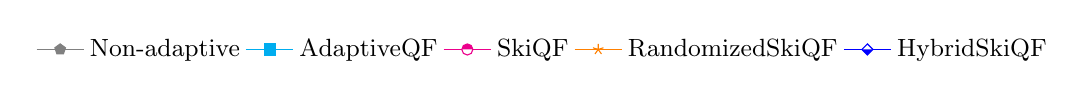
\begin{tikzpicture}
\begin{axis}[hide axis,xmin=0,xmax=1,ymin=0,ymax=1,
scale only axis,width=1cm,height=0.4cm,
legend columns=5,legend cell align=left,
legend style={draw=none,font=\small,at={(0.5,0.5)},anchor=center}]
\addlegendimage{skiqfNonAdaptive}
\addlegendentry{Non-adaptive}
\addlegendimage{skiqfAdaptive}
\addlegendentry{AdaptiveQF}
\addlegendimage{skiqfSki}
\addlegendentry{SkiQF}
\addlegendimage{skiqfRandomized}
\addlegendentry{RandomizedSkiQF}
\addlegendimage{skiqfHybrid}
\addlegendentry{HybridSkiQF}
\end{axis}\end{tikzpicture}
\par\medskip
\begingroup
\pgfmathsetlengthmacro{\skiqfpanelwidth}{(\linewidth-1.6cm-1.3cm)/2}
\begin{tikzpicture}\begin{groupplot}[skiqf axis,
group style={group size=2 by 2,horizontal sep=1.3cm,vertical sep=1.5cm},
scale only axis,width=\skiqfpanelwidth,height=3cm,scaled y ticks=true]
\nextgroupplot[title={Throughput (MOps/s)},
ylabel={Throughput (MOps/s)},
ymin=0,
xlabel={Singleton fraction}]
\addplot[skiqfNonAdaptive,mark size=1.8pt,mark repeat=1] coordinates {(0,2.216873) (0.25,2.203246) (0.5,2.227596) (0.75,2.087827) (1,2.175649)};
\addplot[skiqfAdaptive,mark size=1.8pt,mark repeat=1] coordinates {(0,2.22647) (0.25,2.058051) (0.5,1.764133) (0.75,1.525587) (1,1.211636)};
\addplot[skiqfSki,mark size=1.8pt,mark repeat=1] coordinates {(0,1.501483) (0.25,1.677971) (0.5,1.727754) (0.75,1.944354) (1,2.105198)};
\addplot[skiqfRandomized,mark size=1.8pt,mark repeat=1] coordinates {(0,1.745108) (0.25,1.772908) (0.5,1.718276) (0.75,1.707864) (1,1.675978)};
\addplot[skiqfHybrid,mark size=1.8pt,mark repeat=1] coordinates {(0,2.066307) (0.25,1.846945) (0.5,1.701203) (0.75,1.537137) (1,2.172891)};
\nextgroupplot[title={Observed FPR},
ylabel={Observed FPR},
ymin=0,
xlabel={Singleton fraction}]
\addplot[skiqfNonAdaptive,mark size=1.8pt,mark repeat=1] coordinates {(0,0.0035066) (0.25,0.0034809) (0.5,0.0034749) (0.75,0.0035018) (1,0.0034973)};
\addplot[skiqfAdaptive,mark size=1.8pt,mark repeat=1] coordinates {(0,0.0017558) (0.25,0.0019973) (0.5,0.0023243) (0.75,0.0027963) (1,0.0034938)};
\addplot[skiqfSki,mark size=1.8pt,mark repeat=1] coordinates {(0,0.0035056) (0.25,0.0034798) (0.5,0.003474) (0.75,0.0035002) (1,0.0034973)};
\addplot[skiqfRandomized,mark size=1.8pt,mark repeat=1] coordinates {(0,0.0029458) (0.25,0.0029967) (0.5,0.0031064) (0.75,0.0032714) (1,0.0034963)};
\addplot[skiqfHybrid,mark size=1.8pt,mark repeat=1] coordinates {(0,0.002088) (0.25,0.0022876) (0.5,0.0025447) (0.75,0.0029316) (1,0.0034973)};
\nextgroupplot[title={Adaptations},
ylabel={Adaptations},
ymin=0,
xlabel={Singleton fraction}]
\addplot[skiqfNonAdaptive,mark size=1.8pt,mark repeat=1] coordinates {(0,0) (0.25,0) (0.5,0) (0.75,0) (1,0)};
\addplot[skiqfAdaptive,mark size=1.8pt,mark repeat=1] coordinates {(0,17558) (0.25,19973) (0.5,23243) (0.75,27963) (1,34938)};
\addplot[skiqfSki,mark size=1.8pt,mark repeat=1] coordinates {(0,17528) (0.25,14853) (0.5,11521) (0.75,7054) (1,36)};
\addplot[skiqfRandomized,mark size=1.8pt,mark repeat=1] coordinates {(0,17532) (0.25,16427) (0.5,15344) (0.75,13809) (1,11374)};
\addplot[skiqfHybrid,mark size=1.8pt,mark repeat=1] coordinates {(0,17377) (0.25,19342) (0.5,21991) (0.75,25839) (1,0)};
\nextgroupplot[title={Physical reads (MiB)},
ylabel={Physical reads (MiB)},
ymin=0,
xlabel={Singleton fraction}]
\addplot[skiqfNonAdaptive,mark size=1.8pt,mark repeat=1] coordinates {(0,791.6679688) (0.25,794.7539062) (0.5,801.1328125) (0.75,816.015625) (1,828.2109375)};
\addplot[skiqfAdaptive,mark size=1.8pt,mark repeat=1] coordinates {(0,683.671875) (0.25,780.9804688) (0.5,906.828125) (0.75,1091.105469) (1,1360.703125)};
\addplot[skiqfSki,mark size=1.8pt,mark repeat=1] coordinates {(0,1054.546875) (0.25,1006.304688) (0.5,960.71875) (0.75,905.4296875) (1,807.390625)};
\addplot[skiqfRandomized,mark size=1.8pt,mark repeat=1] coordinates {(0,929.4453125) (0.25,930.9179688) (0.5,943.4296875) (0.75,961.828125) (1,983.6875)};
\addplot[skiqfHybrid,mark size=1.8pt,mark repeat=1] coordinates {(0,755.1796875) (0.25,828.328125) (0.5,933.1445312) (0.75,1085.375) (1,807.2265625)};
\end{groupplot}\end{tikzpicture}\endgroup\end{center}

\begin{center}\small Single-run results; no error bars.\end{center}
\clearpage
\section{Robustness across workload distributions}
Distribution panels and aggregate comparisons follow the paper's robustness study.
\begin{center}
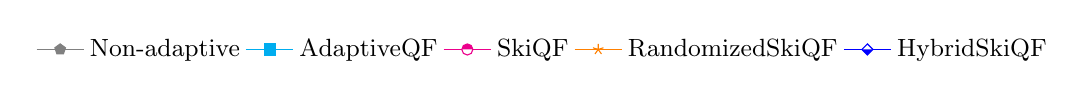
\begin{tikzpicture}
\begin{axis}[hide axis,xmin=0,xmax=1,ymin=0,ymax=1,
scale only axis,width=1cm,height=0.4cm,
legend columns=5,legend cell align=left,
legend style={draw=none,font=\small,at={(0.5,0.5)},anchor=center}]
\addlegendimage{skiqfNonAdaptive}
\addlegendentry{Non-adaptive}
\addlegendimage{skiqfAdaptive}
\addlegendentry{AdaptiveQF}
\addlegendimage{skiqfSki}
\addlegendentry{SkiQF}
\addlegendimage{skiqfRandomized}
\addlegendentry{RandomizedSkiQF}
\addlegendimage{skiqfHybrid}
\addlegendentry{HybridSkiQF}
\end{axis}\end{tikzpicture}
\par\medskip
\begingroup
\pgfmathsetlengthmacro{\skiqfpanelwidth}{(\linewidth-1.6cm-2.0999999999999996cm)/4}
\begin{tikzpicture}\begin{groupplot}[skiqf axis,
group style={group size=4 by 1,horizontal sep=0.7cm,vertical sep=1.5cm},
scale only axis,width=\skiqfpanelwidth,height=3cm,scaled y ticks=true]
\nextgroupplot[title={Uniform},
ylabel={Throughput\\(MOps/sec)},
ymin=0,
xlabel={Queries (millions)},
xmin=0,xmax=10,enlarge x limits=false]
\addplot[skiqfNonAdaptive,mark size=1.8pt,mark repeat=11] coordinates {(0.1,2.030865) (0.2,2.497146) (0.3,1.744239) (0.4,2.00167) (0.5,2.65351) (0.6,2.969764) (0.7,2.219101) (0.8,2.849348) (0.9,3.020066) (1,3.081626) (1.1,2.865159) (1.2,2.956551) (1.3,2.419893) (1.4,2.073362) (1.5,2.097545) (1.6,2.197495) (1.7,1.973438) (1.8,1.908442) (1.9,2.605553) (2,1.862692) (2.1,3.168059) (2.2,2.927243) (2.3,3.062222) (2.4,3.041787) (2.5,3.041678) (2.6,3.112131) (2.7,3.075843) (2.8,2.748984) (2.9,3.044258) (3,2.529372) (3.1,2.752581) (3.2,2.410243) (3.3,1.770835) (3.4,2.042767) (3.5,2.082516) (3.6,1.968068) (3.7,1.685904) (3.8,1.479265) (3.9,1.651607) (4,1.870947) (4.1,1.817746) (4.2,1.663061) (4.3,1.97875) (4.4,2.006212) (4.5,2.154494) (4.6,2.045427) (4.7,2.242427) (4.8,1.738212) (4.9,2.045166) (5,1.874976) (5.1,1.847981) (5.2,1.806826) (5.3,2.145016) (5.4,1.808785) (5.5,2.098452) (5.6,0.962455) (5.7,1.529595) (5.8,2.000026) (5.9,2.18665) (6,1.920353) (6.1,1.9518) (6.2,1.944641) (6.3,1.97263) (6.4,1.746582) (6.5,1.998897) (6.6,2.140367) (6.7,1.880738) (6.8,2.08478) (6.9,1.806682) (7,2.012162) (7.1,1.883858) (7.2,2.071936) (7.3,1.798483) (7.4,2.273847) (7.5,1.936274) (7.6,1.998736) (7.7,2.201887) (7.8,2.193427) (7.9,1.958706) (8,1.870015) (8.1,1.901663) (8.2,2.011282) (8.3,1.980906) (8.4,1.975383) (8.5,2.060362) (8.6,2.15784) (8.7,1.922323) (8.8,1.98216) (8.9,1.996419) (9,1.975108) (9.1,2.037668) (9.2,2.145994) (9.3,1.992617) (9.4,2.1271) (9.5,2.049808) (9.6,1.999639) (9.7,1.641171) (9.8,2.165473) (9.9,1.94022) (10,1.731356)};
\addplot[skiqfAdaptive,mark size=1.8pt,mark repeat=11] coordinates {(0.1,1.185399) (0.2,1.56333) (0.3,1.610159) (0.4,1.349573) (0.5,1.540637) (0.6,1.400337) (0.7,1.205029) (0.8,1.190433) (0.9,1.214942) (1,1.258405) (1.1,1.127794) (1.2,1.196612) (1.3,1.131159) (1.4,1.245065) (1.5,1.257334) (1.6,1.240691) (1.7,1.173355) (1.8,1.164246) (1.9,1.253503) (2,1.192834) (2.1,1.333484) (2.2,1.115178) (2.3,1.265565) (2.4,1.248776) (2.5,1.238284) (2.6,1.275745) (2.7,1.281826) (2.8,1.150182) (2.9,1.188773) (3,1.138431) (3.1,1.139747) (3.2,1.071505) (3.3,1.12686) (3.4,1.040936) (3.5,1.202038) (3.6,1.281355) (3.7,1.168881) (3.8,1.115557) (3.9,1.196803) (4,1.308477) (4.1,1.249974) (4.2,1.140047) (4.3,1.13986) (4.4,1.165202) (4.5,1.225064) (4.6,1.229904) (4.7,1.309035) (4.8,1.15742) (4.9,1.26304) (5,1.167784) (5.1,1.199898) (5.2,1.171778) (5.3,1.430471) (5.4,1.310385) (5.5,1.322114) (5.6,1.260266) (5.7,1.241376) (5.8,1.298737) (5.9,1.239908) (6,1.086468) (6.1,1.273947) (6.2,1.231262) (6.3,1.184877) (6.4,1.270949) (6.5,1.295408) (6.6,1.233104) (6.7,1.125306) (6.8,1.187931) (6.9,1.178635) (7,1.274012) (7.1,1.051219) (7.2,1.216953) (7.3,1.126745) (7.4,1.293784) (7.5,1.094282) (7.6,1.006196) (7.7,1.250734) (7.8,1.292397) (7.9,1.051927) (8,1.164769) (8.1,1.292331) (8.2,1.174692) (8.3,1.159682) (8.4,1.204152) (8.5,1.216562) (8.6,1.25114) (8.7,1.156415) (8.8,1.169371) (8.9,1.152797) (9,1.187215) (9.1,1.206325) (9.2,1.231292) (9.3,1.162684) (9.4,1.296457) (9.5,1.25128) (9.6,1.186123) (9.7,1.253539) (9.8,1.318676) (9.9,1.145623) (10,1.065496)};
\addplot[skiqfSki,mark size=1.8pt,mark repeat=11] coordinates {(0.1,2.266098) (0.2,2.836653) (0.3,2.810902) (0.4,2.589744) (0.5,2.684394) (0.6,2.688839) (0.7,3.014011) (0.8,2.67366) (0.9,3.025639) (1,3.141443) (1.1,2.827066) (1.2,3.02168) (1.3,2.110595) (1.4,2.190528) (1.5,2.131431) (1.6,2.16714) (1.7,2.048855) (1.8,1.964326) (1.9,2.148303) (2,1.009593) (2.1,0.670766) (2.2,0.966174) (2.3,2.052386) (2.4,1.937054) (2.5,2.010161) (2.6,2.08732) (2.7,2.129951) (2.8,1.970993) (2.9,2.064477) (3,1.806275) (3.1,1.978629) (3.2,1.888959) (3.3,1.879215) (3.4,1.99299) (3.5,2.089736) (3.6,2.149145) (3.7,2.079898) (3.8,1.939601) (3.9,1.972362) (4,1.916988) (4.1,2.082905) (4.2,1.958392) (4.3,1.972301) (4.4,1.967408) (4.5,2.099422) (4.6,2.083124) (4.7,2.257601) (4.8,1.910351) (4.9,2.234759) (5,1.94349) (5.1,2.068483) (5.2,2.012367) (5.3,2.453972) (5.4,2.200458) (5.5,2.26068) (5.6,2.160395) (5.7,2.170018) (5.8,2.232207) (5.9,2.155984) (6,1.863269) (6.1,2.176839) (6.2,2.118166) (6.3,2.04442) (6.4,2.126456) (6.5,2.070523) (6.6,2.165009) (6.7,1.937029) (6.8,2.089535) (6.9,2.189323) (7,2.227381) (7.1,1.931587) (7.2,2.039823) (7.3,1.889913) (7.4,2.230329) (7.5,1.947687) (7.6,1.983815) (7.7,2.215523) (7.8,2.242511) (7.9,1.935348) (8,2.043933) (8.1,2.223802) (8.2,2.059003) (8.3,2.007403) (8.4,1.997617) (8.5,2.050324) (8.6,2.195809) (8.7,1.990069) (8.8,2.082107) (8.9,1.965533) (9,2.012774) (9.1,2.058398) (9.2,2.076368) (9.3,2.011664) (9.4,2.173471) (9.5,2.024036) (9.6,1.944696) (9.7,2.072681) (9.8,2.231713) (9.9,2.017919) (10,1.930691)};
\addplot[skiqfRandomized,mark size=1.8pt,mark repeat=11] coordinates {(0.1,1.68672) (0.2,2.203019) (0.3,2.239219) (0.4,2.091905) (0.5,2.08207) (0.6,2.337826) (0.7,2.404249) (0.8,2.437574) (0.9,2.175327) (1,1.768764) (1.1,1.605162) (1.2,1.68428) (1.3,1.569213) (1.4,1.722625) (1.5,1.713248) (1.6,1.715419) (1.7,1.676666) (1.8,1.599639) (1.9,1.731094) (2,1.636699) (2.1,1.850237) (2.2,1.715265) (2.3,1.791661) (2.4,1.794113) (2.5,1.73819) (2.6,1.830524) (2.7,1.776387) (2.8,1.637305) (2.9,1.705859) (3,1.584698) (3.1,1.537047) (3.2,1.686901) (3.3,1.584925) (3.4,1.654088) (3.5,1.729736) (3.6,1.729306) (3.7,1.740314) (3.8,1.58084) (3.9,1.612557) (4,1.797238) (4.1,1.788517) (4.2,1.600839) (4.3,1.675898) (4.4,1.65286) (4.5,1.730394) (4.6,1.705215) (4.7,1.862521) (4.8,1.634205) (4.9,1.847001) (5,1.664358) (5.1,1.683459) (5.2,1.677081) (5.3,1.992666) (5.4,1.690375) (5.5,1.772973) (5.6,1.812498) (5.7,1.799039) (5.8,1.816108) (5.9,1.771145) (6,1.597746) (6.1,1.773276) (6.2,1.714389) (6.3,1.661897) (6.4,1.757693) (6.5,1.853859) (6.6,1.797867) (6.7,1.643028) (6.8,1.745359) (6.9,1.760579) (7,1.78714) (7.1,1.601089) (7.2,1.627467) (7.3,1.517544) (7.4,1.756286) (7.5,1.646674) (7.6,1.637251) (7.7,1.799864) (7.8,1.787682) (7.9,1.604818) (8,1.708798) (8.1,1.649682) (8.2,1.697313) (8.3,1.627193) (8.4,1.721262) (8.5,1.681165) (8.6,1.768922) (8.7,1.655981) (8.8,1.645821) (8.9,1.624623) (9,1.552316) (9.1,1.648877) (9.2,1.740391) (9.3,1.621758) (9.4,1.858727) (9.5,1.639956) (9.6,1.619231) (9.7,1.704269) (9.8,1.823021) (9.9,1.615555) (10,1.603403)};
\addplot[skiqfHybrid,mark size=1.8pt,mark repeat=11] coordinates {(0.1,1.774424) (0.2,2.39547) (0.3,2.370758) (0.4,2.153502) (0.5,1.77955) (0.6,1.933302) (0.7,1.87333) (0.8,2.238838) (0.9,2.534257) (1,2.568101) (1.1,2.3126) (1.2,2.450105) (1.3,1.520138) (1.4,1.349841) (1.5,1.320212) (1.6,1.084978) (1.7,1.275256) (1.8,1.240468) (1.9,1.451005) (2,1.324783) (2.1,1.483176) (2.2,1.34347) (2.3,1.458239) (2.4,1.403898) (2.5,1.164236) (2.6,1.426437) (2.7,1.416712) (2.8,1.337259) (2.9,1.374491) (3,1.270811) (3.1,1.234134) (3.2,1.311312) (3.3,1.325064) (3.4,1.328187) (3.5,1.392938) (3.6,1.424888) (3.7,1.398708) (3.8,1.35898) (3.9,1.403085) (4,1.474427) (4.1,1.431093) (4.2,1.373479) (4.3,1.301154) (4.4,1.336413) (4.5,1.375863) (4.6,1.350555) (4.7,1.508905) (4.8,1.304262) (4.9,1.43651) (5,1.290419) (5.1,1.309725) (5.2,1.330011) (5.3,1.682441) (5.4,1.412571) (5.5,1.481322) (5.6,1.423429) (5.7,1.417503) (5.8,1.482177) (5.9,1.498261) (6,1.315747) (6.1,1.426418) (6.2,1.398213) (6.3,1.334654) (6.4,1.445487) (6.5,1.492604) (6.6,1.466542) (6.7,1.25647) (6.8,1.375893) (6.9,1.430348) (7,1.495366) (7.1,1.239551) (7.2,1.37878) (7.3,1.263535) (7.4,1.469613) (7.5,1.317624) (7.6,1.343287) (7.7,1.470888) (7.8,1.490434) (7.9,1.303245) (8,1.380478) (8.1,1.474026) (8.2,1.348192) (8.3,1.329465) (8.4,1.381872) (8.5,1.373641) (8.6,1.505082) (8.7,1.308373) (8.8,1.360249) (8.9,1.344437) (9,1.289455) (9.1,1.280319) (9.2,1.420608) (9.3,1.28943) (9.4,1.470242) (9.5,1.409552) (9.6,1.35201) (9.7,1.369309) (9.8,1.501053) (9.9,1.335236) (10,1.335395)};
\nextgroupplot[title={Normal},
ymin=0,
xlabel={Queries (millions)},
xmin=0,xmax=10,enlarge x limits=false]
\addplot[skiqfNonAdaptive,mark size=1.8pt,mark repeat=11] coordinates {(0.1,1.760876) (0.2,2.447217) (0.3,2.453435) (0.4,2.844104) (0.5,2.634713) (0.6,3.236876) (0.7,2.941289) (0.8,3.279118) (0.9,3.00583) (1,3.21462) (1.1,2.971613) (1.2,3.426059) (1.3,2.882709) (1.4,3.076036) (1.5,2.879571) (1.6,2.950404) (1.7,2.005161) (1.8,1.623198) (1.9,1.759106) (2,1.73292) (2.1,1.781145) (2.2,1.98814) (2.3,1.863784) (2.4,1.721329) (2.5,1.746568) (2.6,1.781244) (2.7,1.607957) (2.8,1.672208) (2.9,1.909214) (3,1.892902) (3.1,1.738013) (3.2,1.884532) (3.3,1.735576) (3.4,2.011345) (3.5,2.102653) (3.6,1.874511) (3.7,1.87947) (3.8,1.690864) (3.9,1.931239) (4,1.902901) (4.1,1.733226) (4.2,1.789827) (4.3,1.811008) (4.4,1.864244) (4.5,1.722056) (4.6,1.82911) (4.7,2.075017) (4.8,1.858747) (4.9,1.77633) (5,1.744219) (5.1,1.689483) (5.2,1.692648) (5.3,1.628531) (5.4,1.884894) (5.5,1.693418) (5.6,1.650847) (5.7,1.781073) (5.8,1.728166) (5.9,1.692599) (6,1.796334) (6.1,1.849108) (6.2,1.886741) (6.3,1.814379) (6.4,1.694694) (6.5,1.876566) (6.6,1.853906) (6.7,1.732555) (6.8,1.881965) (6.9,1.837948) (7,1.684424) (7.1,1.717513) (7.2,1.720032) (7.3,1.845876) (7.4,1.83945) (7.5,1.672953) (7.6,1.769785) (7.7,1.814334) (7.8,1.727232) (7.9,1.847227) (8,1.740795) (8.1,1.83072) (8.2,1.748236) (8.3,1.628239) (8.4,1.743013) (8.5,1.716346) (8.6,1.874414) (8.7,1.62014) (8.8,1.903253) (8.9,1.561885) (9,1.983245) (9.1,1.877282) (9.2,1.686932) (9.3,1.725891) (9.4,1.755578) (9.5,1.754968) (9.6,1.881929) (9.7,1.91201) (9.8,1.829829) (9.9,1.620117) (10,1.794144)};
\addplot[skiqfAdaptive,mark size=1.8pt,mark repeat=11] coordinates {(0.1,0.710573) (0.2,1.443935) (0.3,1.409182) (0.4,1.565443) (0.5,1.52444) (0.6,1.851588) (0.7,1.605711) (0.8,1.2869) (0.9,1.256078) (1,0.91347) (1.1,1.348221) (1.2,1.601659) (1.3,1.432209) (1.4,1.585369) (1.5,1.566447) (1.6,1.774244) (1.7,1.747171) (1.8,1.694012) (1.9,1.681915) (2,1.441323) (2.1,2.019057) (2.2,2.213218) (2.3,1.789683) (2.4,2.0325) (2.5,2.005482) (2.6,1.88535) (2.7,1.630998) (2.8,2.176563) (2.9,3.038977) (3,2.156152) (3.1,2.494314) (3.2,2.065922) (3.3,2.989425) (3.4,2.952038) (3.5,3.945686) (3.6,3.68992) (3.7,2.994754) (3.8,2.715382) (3.9,3.646524) (4,3.254029) (4.1,3.142382) (4.2,4.442714) (4.3,5.037424) (4.4,3.911305) (4.5,4.030996) (4.6,4.749001) (4.7,4.578289) (4.8,4.280521) (4.9,4.570205) (5,4.175654) (5.1,5.099679) (5.2,4.844114) (5.3,6.638684) (5.4,7.987761) (5.5,4.187608) (5.6,6.840093) (5.7,4.509413) (5.8,6.311926) (5.9,5.485676) (6,4.379561) (6.1,6.708557) (6.2,6.141027) (6.3,7.673259) (6.4,8.953884) (6.5,5.78459) (6.6,8.058204) (6.7,5.142105) (6.8,5.179265) (6.9,4.083207) (7,5.571152) (7.1,5.042528) (7.2,4.65226) (7.3,5.14645) (7.4,5.800024) (7.5,5.09364) (7.6,4.18061) (7.7,4.893381) (7.8,5.813214) (7.9,8.245444) (8,3.749296) (8.1,3.917909) (8.2,6.170098) (8.3,7.535061) (8.4,9.655425) (8.5,5.223177) (8.6,4.722046) (8.7,7.580973) (8.8,7.778181) (8.9,11.515632) (9,11.261599) (9.1,9.289674) (9.2,7.159872) (9.3,6.523486) (9.4,4.447678) (9.5,8.611641) (9.6,10.809711) (9.7,13.054997) (9.8,13.57319) (9.9,11.180905) (10,10.756379)};
\addplot[skiqfSki,mark size=1.8pt,mark repeat=11] coordinates {(0.1,1.646422) (0.2,1.969155) (0.3,1.963342) (0.4,2.261432) (0.5,2.217722) (0.6,2.355334) (0.7,2.172) (0.8,2.344478) (0.9,2.128307) (1,1.7877) (1.1,2.261475) (1.2,2.186765) (1.3,1.458331) (1.4,1.500133) (1.5,1.424106) (1.6,1.458391) (1.7,1.456217) (1.8,1.477571) (1.9,1.525938) (2,1.496739) (2.1,1.640903) (2.2,1.687544) (2.3,1.696283) (2.4,1.564209) (2.5,1.703285) (2.6,1.755102) (2.7,1.787224) (2.8,1.715192) (2.9,2.059078) (3,1.815974) (3.1,1.954085) (3.2,2.220721) (3.3,2.017595) (3.4,2.511962) (3.5,2.520789) (3.6,2.211613) (3.7,2.460478) (3.8,2.010914) (3.9,2.492945) (4,2.724944) (4.1,2.516713) (4.2,2.67958) (4.3,2.576093) (4.4,2.596696) (4.5,2.600107) (4.6,2.746937) (4.7,3.377303) (4.8,3.293842) (4.9,3.562662) (5,2.700802) (5.1,3.379469) (5.2,2.956236) (5.3,3.04827) (5.4,3.76771) (5.5,3.34919) (5.6,3.553271) (5.7,3.70215) (5.8,4.26031) (5.9,3.719962) (6,4.284949) (6.1,5.286632) (6.2,4.086967) (6.3,4.694755) (6.4,3.83629) (6.5,5.018788) (6.6,5.301322) (6.7,4.69377) (6.8,5.019839) (6.9,6.21699) (7,6.298046) (7.1,5.060786) (7.2,6.367868) (7.3,5.697772) (7.4,5.905771) (7.5,5.748827) (7.6,6.235893) (7.7,6.214631) (7.8,6.927643) (7.9,6.505297) (8,6.383954) (8.1,6.506949) (8.2,7.500115) (8.3,6.856592) (8.4,5.52112) (8.5,6.103509) (8.6,7.694708) (8.7,7.374057) (8.8,7.606524) (8.9,6.795028) (9,7.111128) (9.1,10.889903) (9.2,9.400025) (9.3,8.19198) (9.4,7.470941) (9.5,8.61182) (9.6,7.427555) (9.7,7.699606) (9.8,8.967679) (9.9,8.93018) (10,6.925717)};
\addplot[skiqfRandomized,mark size=1.8pt,mark repeat=11] coordinates {(0.1,1.425103) (0.2,2.110857) (0.3,2.23741) (0.4,2.442692) (0.5,2.386715) (0.6,2.706955) (0.7,2.430687) (0.8,2.824079) (0.9,2.690401) (1,2.45821) (1.1,1.944489) (1.2,2.256139) (1.3,2.031598) (1.4,2.174244) (1.5,2.065318) (1.6,1.978268) (1.7,2.060476) (1.8,2.055337) (1.9,2.10954) (2,2.031025) (2.1,2.382071) (2.2,2.388178) (2.3,2.688901) (2.4,2.250694) (2.5,2.134766) (2.6,2.872918) (2.7,2.560296) (2.8,2.652177) (2.9,3.101648) (3,2.933391) (3.1,2.429111) (3.2,2.980337) (3.3,2.884758) (3.4,3.772753) (3.5,3.865207) (3.6,3.328036) (3.7,3.28372) (3.8,3.171858) (3.9,3.80499) (4,3.987442) (4.1,3.153754) (4.2,3.675847) (4.3,4.07872) (4.4,3.767365) (4.5,3.805573) (4.6,4.500438) (4.7,4.983928) (4.8,4.97444) (4.9,4.870532) (5,4.369174) (5.1,5.344691) (5.2,4.272014) (5.3,3.986438) (5.4,5.510917) (5.5,4.649023) (5.6,5.220972) (5.7,5.48905) (5.8,5.876706) (5.9,5.653196) (6,6.287082) (6.1,7.782078) (6.2,6.283425) (6.3,6.822514) (6.4,5.67168) (6.5,7.514348) (6.6,8.098872) (6.7,6.619503) (6.8,7.065142) (6.9,7.436912) (7,7.664785) (7.1,7.121219) (7.2,7.594289) (7.3,8.158035) (7.4,8.697398) (7.5,7.355506) (7.6,9.10052) (7.7,8.575598) (7.8,9.918741) (7.9,9.506176) (8,9.686747) (8.1,7.698678) (8.2,10.033858) (8.3,8.008379) (8.4,8.285669) (8.5,8.715251) (8.6,9.648274) (8.7,9.579974) (8.8,10.836045) (8.9,8.519498) (9,9.4609) (9.1,11.873247) (9.2,11.57118) (9.3,9.767475) (9.4,9.642339) (9.5,10.407968) (9.6,10.129309) (9.7,11.690574) (9.8,10.192557) (9.9,10.062839) (10,8.52984)};
\addplot[skiqfHybrid,mark size=1.8pt,mark repeat=11] coordinates {(0.1,2.151397) (0.2,2.983916) (0.3,2.983657) (0.4,3.451668) (0.5,3.23869) (0.6,3.364126) (0.7,3.45163) (0.8,3.839235) (0.9,3.639079) (1,3.924986) (1.1,1.456202) (1.2,2.113389) (1.3,1.479036) (1.4,1.503204) (1.5,1.353209) (1.6,1.038866) (1.7,1.570665) (1.8,1.544614) (1.9,1.461165) (2,1.626116) (2.1,2.153275) (2.2,2.413863) (2.3,2.25433) (2.4,2.021663) (2.5,2.174979) (2.6,2.589796) (2.7,2.521997) (2.8,2.65177) (2.9,3.343019) (3,2.648574) (3.1,3.038341) (3.2,2.991) (3.3,3.467655) (3.4,4.091937) (3.5,3.838302) (3.6,3.484233) (3.7,4.217926) (3.8,3.34704) (3.9,3.962317) (4,4.103214) (4.1,3.814382) (4.2,4.859377) (4.3,5.20039) (4.4,5.685213) (4.5,4.425418) (4.6,5.351343) (4.7,6.215704) (4.8,5.818563) (4.9,5.831606) (5,5.329516) (5.1,5.753368) (5.2,5.477829) (5.3,6.364401) (5.4,6.97114) (5.5,5.995382) (5.6,6.829445) (5.7,6.228834) (5.8,6.908318) (5.9,7.137109) (6,7.998361) (6.1,8.044669) (6.2,7.943458) (6.3,8.568183) (6.4,8.1948) (6.5,8.839738) (6.6,11.047448) (6.7,9.540743) (6.8,8.909791) (6.9,8.318676) (7,8.86879) (7.1,8.098442) (7.2,8.783886) (7.3,9.911084) (7.4,10.185537) (7.5,10.742659) (7.6,9.80607) (7.7,9.982724) (7.8,11.458953) (7.9,10.072454) (8,9.451915) (8.1,9.545538) (8.2,11.337964) (8.3,10.318244) (8.4,9.954376) (8.5,10.276818) (8.6,12.000978) (8.7,12.976505) (8.8,10.745043) (8.9,12.050179) (9,11.050141) (9.1,14.0205) (9.2,13.184397) (9.3,11.923979) (9.4,11.105958) (9.5,14.338215) (9.6,12.092475) (9.7,8.722009) (9.8,9.48398) (9.9,12.332652) (10,11.701401)};
\nextgroupplot[title={Lognormal},
ymin=0,
xlabel={Queries (millions)},
xmin=0,xmax=10,enlarge x limits=false]
\addplot[skiqfNonAdaptive,mark size=1.8pt,mark repeat=11] coordinates {(0.1,2.12916) (0.2,2.854462) (0.3,1.955026) (0.4,3.309632) (0.5,3.513025) (0.6,3.846036) (0.7,3.580002) (0.8,3.655532) (0.9,3.864151) (1,4.011905) (1.1,3.855627) (1.2,3.731062) (1.3,3.599631) (1.4,3.952141) (1.5,4.069862) (1.6,3.84241) (1.7,3.557299) (1.8,2.731418) (1.9,3.098313) (2,2.928596) (2.1,2.431203) (2.2,2.110672) (2.3,2.81182) (2.4,2.817455) (2.5,2.540179) (2.6,3.048084) (2.7,2.896381) (2.8,2.776347) (2.9,2.748668) (3,2.778369) (3.1,2.851079) (3.2,2.597311) (3.3,2.585145) (3.4,2.471888) (3.5,2.884166) (3.6,2.40422) (3.7,2.889532) (3.8,2.583321) (3.9,2.726586) (4,2.585736) (4.1,2.77938) (4.2,2.813137) (4.3,2.428575) (4.4,2.518) (4.5,2.810561) (4.6,2.719104) (4.7,2.792015) (4.8,2.619018) (4.9,2.501561) (5,3.144711) (5.1,2.962724) (5.2,2.774645) (5.3,2.701119) (5.4,2.645555) (5.5,2.759877) (5.6,2.658723) (5.7,2.75843) (5.8,2.627656) (5.9,2.973942) (6,2.699304) (6.1,2.920505) (6.2,2.626268) (6.3,2.696296) (6.4,2.947179) (6.5,3.032969) (6.6,2.79439) (6.7,2.870352) (6.8,2.627151) (6.9,2.534172) (7,2.755256) (7.1,2.620802) (7.2,2.578483) (7.3,2.682085) (7.4,2.71976) (7.5,2.832061) (7.6,2.590336) (7.7,3.048829) (7.8,2.307907) (7.9,2.517646) (8,1.980995) (8.1,2.049344) (8.2,3.042764) (8.3,2.681282) (8.4,2.696528) (8.5,2.782292) (8.6,2.487381) (8.7,2.976523) (8.8,2.705305) (8.9,2.737247) (9,2.781734) (9.1,2.584224) (9.2,2.804837) (9.3,2.867078) (9.4,2.78206) (9.5,2.616272) (9.6,2.756408) (9.7,2.338978) (9.8,2.039014) (9.9,2.638904) (10,2.373383)};
\addplot[skiqfAdaptive,mark size=1.8pt,mark repeat=11] coordinates {(0.1,1.135482) (0.2,1.758778) (0.3,1.659489) (0.4,1.980389) (0.5,2.065976) (0.6,2.388289) (0.7,1.844234) (0.8,1.627677) (0.9,1.886376) (1,2.047824) (1.1,1.867983) (1.2,2.068645) (1.3,2.056353) (1.4,2.121408) (1.5,2.425381) (1.6,2.254837) (1.7,2.460111) (1.8,2.478457) (1.9,2.754416) (2,2.536035) (2.1,2.58674) (2.2,2.4931) (2.3,2.911991) (2.4,2.459089) (2.5,2.561547) (2.6,3.13901) (2.7,2.958535) (2.8,3.067952) (2.9,3.02079) (3,2.968115) (3.1,3.421236) (3.2,3.014522) (3.3,3.173919) (3.4,2.900594) (3.5,3.337812) (3.6,3.317292) (3.7,3.420158) (3.8,3.662408) (3.9,3.713773) (4,3.436836) (4.1,4.39511) (4.2,4.09498) (4.3,2.931103) (4.4,3.792248) (4.5,4.094564) (4.6,4.393912) (4.7,4.568453) (4.8,5.35273) (4.9,4.153547) (5,4.309667) (5.1,3.382032) (5.2,2.768564) (5.3,4.323564) (5.4,3.761758) (5.5,3.72856) (5.6,3.774319) (5.7,4.289858) (5.8,4.022951) (5.9,3.936148) (6,4.009982) (6.1,5.290686) (6.2,4.977454) (6.3,5.835561) (6.4,5.563312) (6.5,5.296722) (6.6,4.683722) (6.7,5.173227) (6.8,4.074246) (6.9,6.093868) (7,5.188662) (7.1,5.290248) (7.2,5.186417) (7.3,6.017824) (7.4,4.174533) (7.5,6.14886) (7.6,5.638084) (7.7,6.76556) (7.8,5.627769) (7.9,4.62597) (8,5.114303) (8.1,6.897996) (8.2,6.431338) (8.3,6.52409) (8.4,7.189715) (8.5,6.204423) (8.6,6.744828) (8.7,8.154947) (8.8,6.934371) (8.9,6.295067) (9,6.974508) (9.1,6.915344) (9.2,6.482798) (9.3,7.304554) (9.4,6.39946) (9.5,6.511341) (9.6,7.142233) (9.7,7.681514) (9.8,7.49694) (9.9,7.938597) (10,6.704059)};
\addplot[skiqfSki,mark size=1.8pt,mark repeat=11] coordinates {(0.1,1.883671) (0.2,2.212824) (0.3,2.425543) (0.4,2.647311) (0.5,2.402389) (0.6,2.997321) (0.7,2.826788) (0.8,2.826419) (0.9,3.170651) (1,3.232315) (1.1,2.399403) (1.2,2.352887) (1.3,2.322152) (1.4,2.269331) (1.5,2.179018) (1.6,2.262861) (1.7,2.435621) (1.8,2.38826) (1.9,2.155564) (2,2.40982) (2.1,2.41307) (2.2,2.33191) (2.3,2.243716) (2.4,2.551418) (2.5,2.297543) (2.6,2.849159) (2.7,2.790816) (2.8,2.582958) (2.9,2.563864) (3,2.555587) (3.1,2.74983) (3.2,2.793934) (3.3,2.672421) (3.4,2.486622) (3.5,3.202716) (3.6,2.525609) (3.7,2.920516) (3.8,3.068659) (3.9,3.032596) (4,2.739695) (4.1,2.963063) (4.2,3.032675) (4.3,3.019265) (4.4,2.770794) (4.5,3.170351) (4.6,3.116428) (4.7,3.425587) (4.8,3.640111) (4.9,3.110912) (5,3.603371) (5.1,3.319832) (5.2,3.305065) (5.3,3.358312) (5.4,3.306483) (5.5,3.777603) (5.6,3.501671) (5.7,3.616776) (5.8,3.456612) (5.9,3.811257) (6,3.949701) (6.1,3.891452) (6.2,3.514269) (6.3,4.078897) (6.4,4.452436) (6.5,4.203399) (6.6,4.541614) (6.7,4.19503) (6.8,3.732453) (6.9,3.885409) (7,3.931533) (7.1,3.848008) (7.2,3.69844) (7.3,4.173746) (7.4,4.045273) (7.5,4.520272) (7.6,4.06854) (7.7,4.524189) (7.8,4.1827) (7.9,4.240985) (8,4.287654) (8.1,5.23747) (8.2,4.397463) (8.3,4.688468) (8.4,4.711251) (8.5,4.852952) (8.6,4.500428) (8.7,4.92509) (8.8,4.028707) (8.9,4.303627) (9,4.675808) (9.1,4.741502) (9.2,4.664082) (9.3,4.666403) (9.4,5.22265) (9.5,4.636602) (9.6,5.14593) (9.7,4.498611) (9.8,5.271808) (9.9,5.470987) (10,5.012771)};
\addplot[skiqfRandomized,mark size=1.8pt,mark repeat=11] coordinates {(0.1,1.299586) (0.2,2.074423) (0.3,2.106518) (0.4,2.267669) (0.5,2.574016) (0.6,2.878184) (0.7,2.630986) (0.8,2.666302) (0.9,3.013927) (1,2.635815) (1.1,2.087915) (1.2,2.159011) (1.3,2.398491) (1.4,2.363923) (1.5,2.346924) (1.6,1.809112) (1.7,1.361584) (1.8,1.360237) (1.9,1.72537) (2,1.406601) (2.1,1.354771) (2.2,1.343687) (2.3,1.410243) (2.4,1.363629) (2.5,1.587194) (2.6,1.846512) (2.7,1.459053) (2.8,1.715622) (2.9,1.47223) (3,1.763713) (3.1,1.798417) (3.2,1.823098) (3.3,1.486024) (3.4,1.744064) (3.5,1.878483) (3.6,1.463313) (3.7,2.956818) (3.8,2.905304) (3.9,3.168547) (4,3.074308) (4.1,3.3752) (4.2,3.304551) (4.3,2.637869) (4.4,3.328234) (4.5,3.870086) (4.6,3.521789) (4.7,3.469134) (4.8,3.571877) (4.9,3.29277) (5,3.519918) (5.1,3.487301) (5.2,3.252917) (5.3,3.555475) (5.4,3.430117) (5.5,4.023242) (5.6,3.797142) (5.7,3.90708) (5.8,3.602157) (5.9,4.036993) (6,3.9407) (6.1,3.937512) (6.2,3.926239) (6.3,4.48384) (6.4,4.020326) (6.5,4.588677) (6.6,4.865499) (6.7,3.801155) (6.8,3.523594) (6.9,4.625348) (7,4.188249) (7.1,4.065989) (7.2,3.629711) (7.3,4.606516) (7.4,4.635993) (7.5,4.637487) (7.6,4.203868) (7.7,5.123847) (7.8,4.535782) (7.9,4.405152) (8,4.727314) (8.1,5.167826) (8.2,5.314317) (8.3,5.124176) (8.4,5.073885) (8.5,5.408019) (8.6,5.287664) (8.7,4.86404) (8.8,4.827947) (8.9,5.400253) (9,4.773718) (9.1,5.110299) (9.2,5.375755) (9.3,5.278293) (9.4,5.657381) (9.5,5.304465) (9.6,4.9825) (9.7,5.404065) (9.8,5.64222) (9.9,6.202103) (10,5.114879)};
\addplot[skiqfHybrid,mark size=1.8pt,mark repeat=11] coordinates {(0.1,2.043217) (0.2,2.674099) (0.3,2.34825) (0.4,2.69228) (0.5,3.278448) (0.6,3.737362) (0.7,3.263909) (0.8,3.169086) (0.9,3.671444) (1,3.865184) (1.1,1.425707) (1.2,1.887196) (1.3,1.661881) (1.4,1.542364) (1.5,1.659624) (1.6,1.559369) (1.7,1.751213) (1.8,1.752873) (1.9,2.063484) (2,1.908314) (2.1,1.974457) (2.2,1.944124) (2.3,2.081323) (2.4,1.879058) (2.5,1.966849) (2.6,2.579762) (2.7,2.440371) (2.8,2.397673) (2.9,2.382787) (3,2.377384) (3.1,2.644798) (3.2,2.602628) (3.3,2.548973) (3.4,2.50445) (3.5,3.014391) (3.6,2.62071) (3.7,2.747399) (3.8,3.03396) (3.9,2.95045) (4,2.900945) (4.1,3.539649) (4.2,3.111771) (4.3,3.099328) (4.4,3.26505) (4.5,3.700084) (4.6,3.346287) (4.7,4.000089) (4.8,4.436659) (4.9,3.429869) (5,4.682465) (5.1,3.760232) (5.2,3.67704) (5.3,3.878458) (5.4,3.390749) (5.5,3.985707) (5.6,4.391275) (5.7,4.914327) (5.8,4.186399) (5.9,4.308047) (6,4.70538) (6.1,4.754728) (6.2,4.271286) (6.3,4.728614) (6.4,4.909827) (6.5,4.744283) (6.6,4.830656) (6.7,5.23982) (6.8,4.837012) (6.9,4.908007) (7,4.617474) (7.1,4.795) (7.2,4.591908) (7.3,5.831689) (7.4,5.784313) (7.5,5.818066) (7.6,4.946709) (7.7,5.805613) (7.8,5.369689) (7.9,5.404384) (8,5.986534) (8.1,6.071184) (8.2,5.735862) (8.3,5.95286) (8.4,6.177314) (8.5,5.951094) (8.6,6.313053) (8.7,7.130463) (8.8,6.262534) (8.9,5.460326) (9,6.252884) (9.1,6.470079) (9.2,5.803084) (9.3,6.533468) (9.4,6.193617) (9.5,5.900054) (9.6,6.23355) (9.7,5.710028) (9.8,4.939861) (9.9,5.32239) (10,4.861278)};
\nextgroupplot[title={Zipfian},
ymin=0,
xlabel={Queries (millions)},
xmin=0,xmax=10,enlarge x limits=false]
\addplot[skiqfNonAdaptive,mark size=1.8pt,mark repeat=11] coordinates {(0.1,3.319423) (0.2,5.203122) (0.3,5.988403) (0.4,6.446531) (0.5,6.715684) (0.6,7.31048) (0.7,6.897778) (0.8,6.253104) (0.9,6.341162) (1,6.114198) (1.1,6.588399) (1.2,7.715856) (1.3,8.646461) (1.4,8.028259) (1.5,7.336382) (1.6,8.417873) (1.7,9.018392) (1.8,8.41709) (1.9,8.052281) (2,10.17474) (2.1,8.941616) (2.2,9.12748) (2.3,8.284802) (2.4,6.748499) (2.5,7.681076) (2.6,8.864139) (2.7,8.178907) (2.8,9.288352) (2.9,9.038766) (3,8.1441) (3.1,8.832946) (3.2,9.651777) (3.3,8.039468) (3.4,8.14741) (3.5,8.063491) (3.6,8.606402) (3.7,8.781331) (3.8,8.634278) (3.9,8.382657) (4,7.90921) (4.1,9.252777) (4.2,9.599846) (4.3,9.35207) (4.4,8.734004) (4.5,8.269592) (4.6,8.501684) (4.7,7.355961) (4.8,5.359387) (4.9,5.82044) (5,5.493614) (5.1,4.463476) (5.2,6.164352) (5.3,5.863001) (5.4,6.908864) (5.5,5.680423) (5.6,5.03444) (5.7,6.414695) (5.8,6.339779) (5.9,5.872872) (6,6.45977) (6.1,6.655751) (6.2,5.732823) (6.3,6.723947) (6.4,6.766546) (6.5,6.624539) (6.6,6.679141) (6.7,5.9609) (6.8,6.898975) (6.9,5.876518) (7,7.063973) (7.1,6.036729) (7.2,5.941021) (7.3,5.969193) (7.4,5.889847) (7.5,6.289523) (7.6,6.553761) (7.7,6.29422) (7.8,6.779978) (7.9,6.159482) (8,6.585936) (8.1,5.330765) (8.2,6.534174) (8.3,6.920195) (8.4,6.665705) (8.5,5.548152) (8.6,5.117945) (8.7,6.548163) (8.8,6.6183) (8.9,6.692717) (9,6.7821) (9.1,5.790233) (9.2,6.018783) (9.3,7.202758) (9.4,6.404135) (9.5,6.77111) (9.6,6.245832) (9.7,7.035358) (9.8,6.131456) (9.9,5.973638) (10,6.599055)};
\addplot[skiqfAdaptive,mark size=1.8pt,mark repeat=11] coordinates {(0.1,1.70145) (0.2,3.077242) (0.3,3.681669) (0.4,4.022558) (0.5,4.161589) (0.6,4.895893) (0.7,4.422204) (0.8,4.207348) (0.9,5.300899) (1,4.804588) (1.1,4.448056) (1.2,5.158659) (1.3,5.914604) (1.4,5.021351) (1.5,4.732056) (1.6,5.840886) (1.7,6.070667) (1.8,5.681566) (1.9,4.032829) (2,5.122171) (2.1,4.928754) (2.2,4.538629) (2.3,4.689904) (2.4,4.430848) (2.5,4.109672) (2.6,4.58854) (2.7,4.591361) (2.8,5.151003) (2.9,5.005485) (3,4.63708) (3.1,5.181977) (3.2,4.947749) (3.3,4.408435) (3.4,3.855876) (3.5,4.238931) (3.6,4.655015) (3.7,5.066327) (3.8,5.057764) (3.9,5.438369) (4,4.801312) (4.1,6.13029) (4.2,5.949532) (4.3,5.563686) (4.4,5.325803) (4.5,4.948824) (4.6,4.959769) (4.7,5.567647) (4.8,4.739972) (4.9,5.953442) (5,5.115904) (5.1,5.192299) (5.2,4.420123) (5.3,4.751459) (5.4,5.944691) (5.5,5.192338) (5.6,5.757878) (5.7,5.54299) (5.8,5.592591) (5.9,5.704328) (6,5.17361) (6.1,5.870691) (6.2,5.120892) (6.3,5.809381) (6.4,6.447933) (6.5,5.981333) (6.6,5.286184) (6.7,5.254264) (6.8,5.633431) (6.9,5.684434) (7,4.978916) (7.1,4.720745) (7.2,5.224355) (7.3,5.731499) (7.4,5.810429) (7.5,6.022657) (7.6,5.966716) (7.7,5.977369) (7.8,6.283941) (7.9,7.157782) (8,7.421052) (8.1,5.080742) (8.2,6.602555) (8.3,7.617767) (8.4,6.565408) (8.5,7.430311) (8.6,6.151464) (8.7,6.617015) (8.8,6.912909) (8.9,6.986424) (9,6.90205) (9.1,5.800885) (9.2,6.128517) (9.3,6.336451) (9.4,6.152519) (9.5,6.905206) (9.6,5.990236) (9.7,6.06837) (9.8,5.999078) (9.9,6.201652) (10,6.257787)};
\addplot[skiqfSki,mark size=1.8pt,mark repeat=11] coordinates {(0.1,2.352977) (0.2,3.887864) (0.3,4.284541) (0.4,5.399523) (0.5,5.435972) (0.6,6.039647) (0.7,5.677765) (0.8,5.602842) (0.9,7.238133) (1,6.251673) (1.1,5.975601) (1.2,6.476311) (1.3,5.79941) (1.4,5.717483) (1.5,6.064315) (1.6,7.476376) (1.7,7.943838) (1.8,6.188175) (1.9,5.930091) (2,8.464432) (2.1,7.661734) (2.2,7.888083) (2.3,7.891413) (2.4,7.682616) (2.5,7.256556) (2.6,8.131626) (2.7,7.305734) (2.8,8.399541) (2.9,8.650231) (3,7.754302) (3.1,8.051195) (3.2,8.641823) (3.3,7.088926) (3.4,5.006263) (3.5,5.334943) (3.6,5.48154) (3.7,6.171311) (3.8,5.875799) (3.9,5.336591) (4,6.06819) (4.1,6.450997) (4.2,6.113783) (4.3,6.514346) (4.4,6.829486) (4.5,5.647287) (4.6,5.8206) (4.7,5.707536) (4.8,5.798348) (4.9,6.388336) (5,6.284469) (5.1,5.847991) (5.2,6.136833) (5.3,5.219432) (5.4,6.551982) (5.5,5.744441) (5.6,5.804329) (5.7,5.860076) (5.8,6.42344) (5.9,5.001306) (6,5.923741) (6.1,6.696493) (6.2,4.978193) (6.3,6.206868) (6.4,6.579959) (6.5,5.700997) (6.6,6.362184) (6.7,6.466012) (6.8,6.750393) (6.9,5.420023) (7,6.253432) (7.1,6.681863) (7.2,6.235396) (7.3,7.031156) (7.4,6.479051) (7.5,6.699964) (7.6,6.345529) (7.7,5.980712) (7.8,6.861147) (7.9,7.154059) (8,7.807352) (8.1,5.723289) (8.2,7.764983) (8.3,7.045001) (8.4,7.258519) (8.5,8.189478) (8.6,6.322506) (8.7,6.456978) (8.8,8.462983) (8.9,7.132946) (9,7.32888) (9.1,5.354445) (9.2,6.230968) (9.3,6.874428) (9.4,6.163861) (9.5,6.689198) (9.6,6.823508) (9.7,7.809576) (9.8,5.952814) (9.9,7.0991) (10,6.276475)};
\addplot[skiqfRandomized,mark size=1.8pt,mark repeat=11] coordinates {(0.1,2.253715) (0.2,3.733203) (0.3,4.085308) (0.4,4.811674) (0.5,5.007314) (0.6,5.055611) (0.7,4.452223) (0.8,5.099848) (0.9,5.403315) (1,5.853212) (1.1,5.61847) (1.2,5.745626) (1.3,7.107421) (1.4,6.086322) (1.5,5.784068) (1.6,7.052049) (1.7,6.380044) (1.8,6.56465) (1.9,6.399175) (2,7.857412) (2.1,7.396282) (2.2,7.649205) (2.3,7.635901) (2.4,7.216609) (2.5,7.101773) (2.6,7.214058) (2.7,6.61798) (2.8,6.192423) (2.9,5.783357) (3,5.23776) (3.1,5.663729) (3.2,6.305873) (3.3,4.897005) (3.4,5.201458) (3.5,5.459673) (3.6,4.841744) (3.7,5.778939) (3.8,5.522192) (3.9,5.308631) (4,5.734381) (4.1,6.204278) (4.2,6.735402) (4.3,6.266448) (4.4,5.757806) (4.5,5.330883) (4.6,5.163081) (4.7,6.415157) (4.8,5.106813) (4.9,6.294597) (5,5.307435) (5.1,5.368512) (5.2,5.327583) (5.3,5.046208) (5.4,5.341072) (5.5,5.171803) (5.6,5.283156) (5.7,5.857629) (5.8,5.934394) (5.9,5.631774) (6,5.276531) (6.1,6.176096) (6.2,5.209137) (6.3,6.026894) (6.4,6.12544) (6.5,6.020843) (6.6,5.684009) (6.7,5.71643) (6.8,6.562973) (6.9,5.462567) (7,6.509377) (7.1,6.143545) (7.2,6.04781) (7.3,6.712558) (7.4,6.399599) (7.5,6.740637) (7.6,5.983451) (7.7,6.024784) (7.8,6.296727) (7.9,7.099565) (8,7.091982) (8.1,5.901967) (8.2,6.001668) (8.3,6.147705) (8.4,5.381065) (8.5,6.885873) (8.6,6.517026) (8.7,6.66116) (8.8,7.732593) (8.9,7.309446) (9,6.866492) (9.1,5.250828) (9.2,5.293598) (9.3,6.361354) (9.4,6.293476) (9.5,7.645306) (9.6,6.415195) (9.7,7.686914) (9.8,6.073631) (9.9,6.727506) (10,6.103391)};
\addplot[skiqfHybrid,mark size=1.8pt,mark repeat=11] coordinates {(0.1,3.460745) (0.2,5.012314) (0.3,5.884828) (0.4,6.325207) (0.5,6.718633) (0.6,7.232287) (0.7,6.718969) (0.8,6.450753) (0.9,7.866803) (1,7.781889) (1.1,2.312241) (1.2,3.638722) (1.3,4.601772) (1.4,4.470333) (1.5,4.283871) (1.6,5.165967) (1.7,5.710664) (1.8,4.980447) (1.9,4.913559) (2,6.162446) (2.1,5.880844) (2.2,5.714655) (2.3,5.6607) (2.4,4.655077) (2.5,3.932638) (2.6,4.344414) (2.7,4.025128) (2.8,4.586627) (2.9,4.425327) (3,4.52852) (3.1,4.652846) (3.2,4.923084) (3.3,4.273775) (3.4,3.942592) (3.5,3.982086) (3.6,4.160176) (3.7,4.602191) (3.8,4.194465) (3.9,4.678162) (4,3.81029) (4.1,4.722679) (4.2,4.634653) (4.3,4.987342) (4.4,4.680415) (4.5,4.468105) (4.6,4.551225) (4.7,4.266243) (4.8,4.554969) (4.9,5.379083) (5,4.758663) (5.1,4.9648) (5.2,4.327394) (5.3,4.445597) (5.4,5.136973) (5.5,4.969069) (5.6,5.411669) (5.7,4.908307) (5.8,4.96867) (5.9,4.982499) (6,4.967216) (6.1,5.598118) (6.2,4.663557) (6.3,5.325642) (6.4,6.30808) (6.5,5.634781) (6.6,5.071211) (6.7,5.272618) (6.8,5.646822) (6.9,5.737648) (7,5.59852) (7.1,5.405593) (7.2,5.58098) (7.3,6.910125) (7.4,5.504909) (7.5,5.396878) (7.6,5.482295) (7.7,5.428152) (7.8,6.103322) (7.9,6.547681) (8,6.955921) (8.1,5.087504) (8.2,6.669922) (8.3,6.58865) (8.4,6.241) (8.5,7.23588) (8.6,5.474874) (8.7,6.45727) (8.8,6.745003) (8.9,6.927064) (9,6.393223) (9.1,5.143371) (9.2,5.542038) (9.3,6.074451) (9.4,5.88617) (9.5,6.564973) (9.6,5.661932) (9.7,6.4777) (9.8,5.620353) (9.9,5.802313) (10,5.863839)};
\end{groupplot}\end{tikzpicture}\endgroup\end{center}

\begin{center}\small Instantaneous database query throughput. Higher is better.\end{center}
\begin{center}
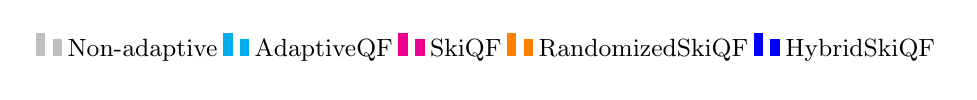
\begin{tikzpicture}
\begin{axis}[hide axis,xmin=0,xmax=1,ymin=0,ymax=1,
scale only axis,width=1cm,height=0.4cm,
legend columns=5,legend cell align=left,
legend style={draw=none,font=\small,at={(0.5,0.5)},anchor=center}]
\addlegendimage{ybar legend,/tikz/ybar,skiqfNonAdaptiveBar}
\addlegendentry{Non-adaptive}
\addlegendimage{ybar legend,/tikz/ybar,skiqfAdaptiveBar}
\addlegendentry{AdaptiveQF}
\addlegendimage{ybar legend,/tikz/ybar,skiqfSkiBar}
\addlegendentry{SkiQF}
\addlegendimage{ybar legend,/tikz/ybar,skiqfRandomizedBar}
\addlegendentry{RandomizedSkiQF}
\addlegendimage{ybar legend,/tikz/ybar,skiqfHybridBar}
\addlegendentry{HybridSkiQF}
\end{axis}\end{tikzpicture}
\par\medskip
\begingroup
\pgfmathsetlengthmacro{\skiqfpanelwidth}{(\linewidth-1.6cm-0.0cm)/1}
\begin{tikzpicture}\begin{groupplot}[skiqf axis,
group style={group size=1 by 1,horizontal sep=0.7cm,vertical sep=1.5cm},
scale only axis,width=\skiqfpanelwidth,height=3cm,scaled y ticks=true]
\nextgroupplot[title={Overall query throughput},
ylabel={Throughput\\(MOps/sec)},
ymin=0,
ybar=0,bar width=5pt,enlarge x limits=false,
xmin=-0.5,xmax=3.5,
xtick={0,1,2,3},
xticklabels={Uniform,Normal,Lognormal,Zipfian},
x tick label style={rotate=45,anchor=east,font=\scriptsize}]
\addplot[skiqfNonAdaptiveBar,mark size=1.8pt,mark repeat=1] coordinates {(0,2.068739) (1,1.895934) (2,2.764757) (3,6.790382)};
\addplot[skiqfAdaptiveBar,mark size=1.8pt,mark repeat=1] coordinates {(0,1.211388) (1,3.02368) (2,3.51782) (3,5.17478)};
\addplot[skiqfSkiBar,mark size=1.8pt,mark repeat=1] coordinates {(0,2.035416) (1,2.938368) (2,3.241766) (3,6.247072)};
\addplot[skiqfRandomizedBar,mark size=1.8pt,mark repeat=1] coordinates {(0,1.731598) (1,3.965002) (2,2.811685) (3,5.818481)};
\addplot[skiqfHybridBar,mark size=1.8pt,mark repeat=1] coordinates {(0,1.43449) (1,4.129935) (2,3.324736) (3,5.138479)};
\end{groupplot}\end{tikzpicture}\endgroup\end{center}

\begin{center}\small Final cumulative throughput; higher is better.\end{center}
\clearpage
\begin{center}
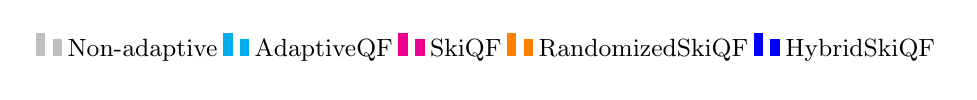
\begin{tikzpicture}
\begin{axis}[hide axis,xmin=0,xmax=1,ymin=0,ymax=1,
scale only axis,width=1cm,height=0.4cm,
legend columns=5,legend cell align=left,
legend style={draw=none,font=\small,at={(0.5,0.5)},anchor=center}]
\addlegendimage{ybar legend,/tikz/ybar,skiqfNonAdaptiveBar}
\addlegendentry{Non-adaptive}
\addlegendimage{ybar legend,/tikz/ybar,skiqfAdaptiveBar}
\addlegendentry{AdaptiveQF}
\addlegendimage{ybar legend,/tikz/ybar,skiqfSkiBar}
\addlegendentry{SkiQF}
\addlegendimage{ybar legend,/tikz/ybar,skiqfRandomizedBar}
\addlegendentry{RandomizedSkiQF}
\addlegendimage{ybar legend,/tikz/ybar,skiqfHybridBar}
\addlegendentry{HybridSkiQF}
\end{axis}\end{tikzpicture}
\par\medskip
\begingroup
\pgfmathsetlengthmacro{\skiqfpanelwidth}{(\linewidth-1.6cm-0.0cm)/1}
\begin{tikzpicture}\begin{groupplot}[skiqf axis,
group style={group size=1 by 1,horizontal sep=0.7cm,vertical sep=1.5cm},
scale only axis,width=\skiqfpanelwidth,height=3cm,scaled y ticks=true]
\nextgroupplot[title={Overall disk I/O},
ylabel={Bytes read\\(GiB)},
ymin=0,
ybar=0,bar width=5pt,enlarge x limits=false,
xmin=-0.5,xmax=3.5,
xtick={0,1,2,3},
xticklabels={Uniform,Normal,Lognormal,Zipfian},
x tick label style={rotate=45,anchor=east,font=\scriptsize}]
\addplot[skiqfNonAdaptiveBar,mark size=1.8pt,mark repeat=1] coordinates {(0,0.8140220642) (1,0.6193466187) (2,0.5996246338) (3,0.2178497314)};
\addplot[skiqfAdaptiveBar,mark size=1.8pt,mark repeat=1] coordinates {(0,1.334709167) (1,0.2655448914) (2,0.3834266663) (3,0.2697715759)};
\addplot[skiqfSkiBar,mark size=1.8pt,mark repeat=1] coordinates {(0,0.7921600342) (1,0.3638153076) (2,0.4488105774) (3,0.2252578735)};
\addplot[skiqfRandomizedBar,mark size=1.8pt,mark repeat=1] coordinates {(0,0.9665985107) (1,0.3255844116) (2,0.4227333069) (3,0.2389945984)};
\addplot[skiqfHybridBar,mark size=1.8pt,mark repeat=1] coordinates {(0,0.7920684814) (1,0.3141288757) (2,0.421672821) (3,0.2704772949)};
\end{groupplot}\end{tikzpicture}\endgroup\end{center}

\begin{center}\small Database plus reverse-map physical reads. Lower is better.\end{center}
\clearpage
\begin{center}
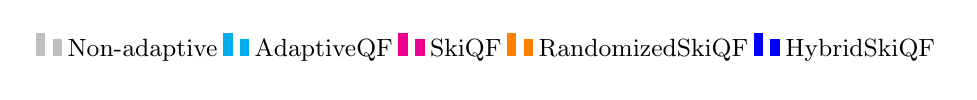
\begin{tikzpicture}
\begin{axis}[hide axis,xmin=0,xmax=1,ymin=0,ymax=1,
scale only axis,width=1cm,height=0.4cm,
legend columns=5,legend cell align=left,
legend style={draw=none,font=\small,at={(0.5,0.5)},anchor=center}]
\addlegendimage{ybar legend,/tikz/ybar,skiqfNonAdaptiveBar}
\addlegendentry{Non-adaptive}
\addlegendimage{ybar legend,/tikz/ybar,skiqfAdaptiveBar}
\addlegendentry{AdaptiveQF}
\addlegendimage{ybar legend,/tikz/ybar,skiqfSkiBar}
\addlegendentry{SkiQF}
\addlegendimage{ybar legend,/tikz/ybar,skiqfRandomizedBar}
\addlegendentry{RandomizedSkiQF}
\addlegendimage{ybar legend,/tikz/ybar,skiqfHybridBar}
\addlegendentry{HybridSkiQF}
\end{axis}\end{tikzpicture}
\par\medskip
\begingroup
\pgfmathsetlengthmacro{\skiqfpanelwidth}{(\linewidth-1.6cm-2.0999999999999996cm)/4}
\begin{tikzpicture}\begin{groupplot}[skiqf axis,
group style={group size=4 by 2,horizontal sep=0.7cm,vertical sep=1.5cm},
scale only axis,width=\skiqfpanelwidth,height=3cm,scaled y ticks=true]
\nextgroupplot[title={Uniform},
ylabel={Bytes read\\(GiB)},
ymin=0,
ybar=0,bar width=5pt,enlarge x limits=false,
xmin=-0.5,xmax=0.5,
xtick={0},
xticklabels={},
x tick label style={rotate=45,anchor=east,font=\scriptsize}]
\addplot[skiqfNonAdaptiveBar,mark size=1.8pt,mark repeat=1] coordinates {(0,0.8140220642)};
\addplot[skiqfAdaptiveBar,mark size=1.8pt,mark repeat=1] coordinates {(0,0.7919006348)};
\addplot[skiqfSkiBar,mark size=1.8pt,mark repeat=1] coordinates {(0,0.7913894653)};
\addplot[skiqfRandomizedBar,mark size=1.8pt,mark repeat=1] coordinates {(0,0.791595459)};
\addplot[skiqfHybridBar,mark size=1.8pt,mark repeat=1] coordinates {(0,0.7920303345)};
\nextgroupplot[title={Normal},
ymin=0,
ybar=0,bar width=5pt,enlarge x limits=false,
xmin=-0.5,xmax=0.5,
xtick={0},
xticklabels={},
x tick label style={rotate=45,anchor=east,font=\scriptsize}]
\addplot[skiqfNonAdaptiveBar,mark size=1.8pt,mark repeat=1] coordinates {(0,0.6193466187)};
\addplot[skiqfAdaptiveBar,mark size=1.8pt,mark repeat=1] coordinates {(0,0.1583366394)};
\addplot[skiqfSkiBar,mark size=1.8pt,mark repeat=1] coordinates {(0,0.2613334656)};
\addplot[skiqfRandomizedBar,mark size=1.8pt,mark repeat=1] coordinates {(0,0.2221488953)};
\addplot[skiqfHybridBar,mark size=1.8pt,mark repeat=1] coordinates {(0,0.2088661194)};
\nextgroupplot[title={Lognormal},
ymin=0,
ybar=0,bar width=5pt,enlarge x limits=false,
xmin=-0.5,xmax=0.5,
xtick={0},
xticklabels={},
x tick label style={rotate=45,anchor=east,font=\scriptsize}]
\addplot[skiqfNonAdaptiveBar,mark size=1.8pt,mark repeat=1] coordinates {(0,0.5996246338)};
\addplot[skiqfAdaptiveBar,mark size=1.8pt,mark repeat=1] coordinates {(0,0.2284736633)};
\addplot[skiqfSkiBar,mark size=1.8pt,mark repeat=1] coordinates {(0,0.3428878784)};
\addplot[skiqfRandomizedBar,mark size=1.8pt,mark repeat=1] coordinates {(0,0.3012886047)};
\addplot[skiqfHybridBar,mark size=1.8pt,mark repeat=1] coordinates {(0,0.2723083496)};
\nextgroupplot[title={Zipfian},
ymin=0,
ybar=0,bar width=5pt,enlarge x limits=false,
xmin=-0.5,xmax=0.5,
xtick={0},
xticklabels={},
x tick label style={rotate=45,anchor=east,font=\scriptsize}]
\addplot[skiqfNonAdaptiveBar,mark size=1.8pt,mark repeat=1] coordinates {(0,0.2178497314)};
\addplot[skiqfAdaptiveBar,mark size=1.8pt,mark repeat=1] coordinates {(0,0.161113739)};
\addplot[skiqfSkiBar,mark size=1.8pt,mark repeat=1] coordinates {(0,0.1901359558)};
\addplot[skiqfRandomizedBar,mark size=1.8pt,mark repeat=1] coordinates {(0,0.180683136)};
\addplot[skiqfHybridBar,mark size=1.8pt,mark repeat=1] coordinates {(0,0.1688728333)};
\nextgroupplot[title={Uniform},
ylabel={False positives\\(millions)},
ymin=0,
ybar=0,bar width=5pt,enlarge x limits=false,
xmin=-0.5,xmax=0.5,
xtick={0},
xticklabels={},
x tick label style={rotate=45,anchor=east,font=\scriptsize}]
\addplot[skiqfNonAdaptiveBar,mark size=1.8pt,mark repeat=1] coordinates {(0,0.034946)};
\addplot[skiqfAdaptiveBar,mark size=1.8pt,mark repeat=1] coordinates {(0,0.034907)};
\addplot[skiqfSkiBar,mark size=1.8pt,mark repeat=1] coordinates {(0,0.034946)};
\addplot[skiqfRandomizedBar,mark size=1.8pt,mark repeat=1] coordinates {(0,0.034937)};
\addplot[skiqfHybridBar,mark size=1.8pt,mark repeat=1] coordinates {(0,0.034946)};
\nextgroupplot[title={Normal},
ymin=0,
ybar=0,bar width=5pt,enlarge x limits=false,
xmin=-0.5,xmax=0.5,
xtick={0},
xticklabels={},
x tick label style={rotate=45,anchor=east,font=\scriptsize}]
\addplot[skiqfNonAdaptiveBar,mark size=1.8pt,mark repeat=1] coordinates {(0,0.034702)};
\addplot[skiqfAdaptiveBar,mark size=1.8pt,mark repeat=1] coordinates {(0,0.006901)};
\addplot[skiqfSkiBar,mark size=1.8pt,mark repeat=1] coordinates {(0,0.013454)};
\addplot[skiqfRandomizedBar,mark size=1.8pt,mark repeat=1] coordinates {(0,0.011345)};
\addplot[skiqfHybridBar,mark size=1.8pt,mark repeat=1] coordinates {(0,0.010295)};
\nextgroupplot[title={Lognormal},
ymin=0,
ybar=0,bar width=5pt,enlarge x limits=false,
xmin=-0.5,xmax=0.5,
xtick={0},
xticklabels={},
x tick label style={rotate=45,anchor=east,font=\scriptsize}]
\addplot[skiqfNonAdaptiveBar,mark size=1.8pt,mark repeat=1] coordinates {(0,0.034952)};
\addplot[skiqfAdaptiveBar,mark size=1.8pt,mark repeat=1] coordinates {(0,0.010057)};
\addplot[skiqfSkiBar,mark size=1.8pt,mark repeat=1] coordinates {(0,0.016895)};
\addplot[skiqfRandomizedBar,mark size=1.8pt,mark repeat=1] coordinates {(0,0.014664)};
\addplot[skiqfHybridBar,mark size=1.8pt,mark repeat=1] coordinates {(0,0.013178)};
\nextgroupplot[title={Zipfian},
ymin=0,
ybar=0,bar width=5pt,enlarge x limits=false,
xmin=-0.5,xmax=0.5,
xtick={0},
xticklabels={},
x tick label style={rotate=45,anchor=east,font=\scriptsize}]
\addplot[skiqfNonAdaptiveBar,mark size=1.8pt,mark repeat=1] coordinates {(0,0.028093)};
\addplot[skiqfAdaptiveBar,mark size=1.8pt,mark repeat=1] coordinates {(0,0.006974)};
\addplot[skiqfSkiBar,mark size=1.8pt,mark repeat=1] coordinates {(0,0.009172)};
\addplot[skiqfRandomizedBar,mark size=1.8pt,mark repeat=1] coordinates {(0,0.008445)};
\addplot[skiqfHybridBar,mark size=1.8pt,mark repeat=1] coordinates {(0,0.00926)};
\end{groupplot}\end{tikzpicture}\endgroup\end{center}

\begin{center}\small Database I/O and false positives. Lower is better.\end{center}
\clearpage
\begin{center}
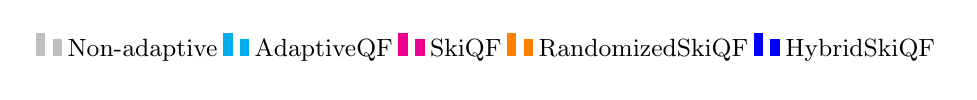
\begin{tikzpicture}
\begin{axis}[hide axis,xmin=0,xmax=1,ymin=0,ymax=1,
scale only axis,width=1cm,height=0.4cm,
legend columns=5,legend cell align=left,
legend style={draw=none,font=\small,at={(0.5,0.5)},anchor=center}]
\addlegendimage{ybar legend,/tikz/ybar,skiqfNonAdaptiveBar}
\addlegendentry{Non-adaptive}
\addlegendimage{ybar legend,/tikz/ybar,skiqfAdaptiveBar}
\addlegendentry{AdaptiveQF}
\addlegendimage{ybar legend,/tikz/ybar,skiqfSkiBar}
\addlegendentry{SkiQF}
\addlegendimage{ybar legend,/tikz/ybar,skiqfRandomizedBar}
\addlegendentry{RandomizedSkiQF}
\addlegendimage{ybar legend,/tikz/ybar,skiqfHybridBar}
\addlegendentry{HybridSkiQF}
\end{axis}\end{tikzpicture}
\par\medskip
\begingroup
\pgfmathsetlengthmacro{\skiqfpanelwidth}{(\linewidth-1.6cm-2.0999999999999996cm)/4}
\begin{tikzpicture}\begin{groupplot}[skiqf axis,
group style={group size=4 by 2,horizontal sep=0.7cm,vertical sep=1.5cm},
scale only axis,width=\skiqfpanelwidth,height=3cm,scaled y ticks=true]
\nextgroupplot[title={Uniform},
ylabel={Bytes read\\(GiB)},
ymin=0,
ybar=0,bar width=5pt,enlarge x limits=false,
xmin=-0.5,xmax=0.5,
xtick={0},
xticklabels={},
x tick label style={rotate=45,anchor=east,font=\scriptsize}]
\addplot[skiqfNonAdaptiveBar,mark size=1.8pt,mark repeat=1] coordinates {(0,0)};
\addplot[skiqfAdaptiveBar,mark size=1.8pt,mark repeat=1] coordinates {(0,0.5428085327)};
\addplot[skiqfSkiBar,mark size=1.8pt,mark repeat=1] coordinates {(0,0.0007705688477)};
\addplot[skiqfRandomizedBar,mark size=1.8pt,mark repeat=1] coordinates {(0,0.1750030518)};
\addplot[skiqfHybridBar,mark size=1.8pt,mark repeat=1] coordinates {(0,3.814697266e-05)};
\nextgroupplot[title={Normal},
ymin=0,
ybar=0,bar width=5pt,enlarge x limits=false,
xmin=-0.5,xmax=0.5,
xtick={0},
xticklabels={},
x tick label style={rotate=45,anchor=east,font=\scriptsize}]
\addplot[skiqfNonAdaptiveBar,mark size=1.8pt,mark repeat=1] coordinates {(0,0)};
\addplot[skiqfAdaptiveBar,mark size=1.8pt,mark repeat=1] coordinates {(0,0.107208252)};
\addplot[skiqfSkiBar,mark size=1.8pt,mark repeat=1] coordinates {(0,0.102481842)};
\addplot[skiqfRandomizedBar,mark size=1.8pt,mark repeat=1] coordinates {(0,0.1034355164)};
\addplot[skiqfHybridBar,mark size=1.8pt,mark repeat=1] coordinates {(0,0.1052627563)};
\nextgroupplot[title={Lognormal},
ymin=0,
ybar=0,bar width=5pt,enlarge x limits=false,
xmin=-0.5,xmax=0.5,
xtick={0},
xticklabels={},
x tick label style={rotate=45,anchor=east,font=\scriptsize}]
\addplot[skiqfNonAdaptiveBar,mark size=1.8pt,mark repeat=1] coordinates {(0,0)};
\addplot[skiqfAdaptiveBar,mark size=1.8pt,mark repeat=1] coordinates {(0,0.1549530029)};
\addplot[skiqfSkiBar,mark size=1.8pt,mark repeat=1] coordinates {(0,0.105922699)};
\addplot[skiqfRandomizedBar,mark size=1.8pt,mark repeat=1] coordinates {(0,0.1214447021)};
\addplot[skiqfHybridBar,mark size=1.8pt,mark repeat=1] coordinates {(0,0.1493644714)};
\nextgroupplot[title={Zipfian},
ymin=0,
ybar=0,bar width=5pt,enlarge x limits=false,
xmin=-0.5,xmax=0.5,
xtick={0},
xticklabels={},
x tick label style={rotate=45,anchor=east,font=\scriptsize}]
\addplot[skiqfNonAdaptiveBar,mark size=1.8pt,mark repeat=1] coordinates {(0,0)};
\addplot[skiqfAdaptiveBar,mark size=1.8pt,mark repeat=1] coordinates {(0,0.1086578369)};
\addplot[skiqfSkiBar,mark size=1.8pt,mark repeat=1] coordinates {(0,0.03512191772)};
\addplot[skiqfRandomizedBar,mark size=1.8pt,mark repeat=1] coordinates {(0,0.0583114624)};
\addplot[skiqfHybridBar,mark size=1.8pt,mark repeat=1] coordinates {(0,0.1016044617)};
\nextgroupplot[title={Uniform},
ylabel={Adaptations\\(millions)},
ymin=0,
ybar=0,bar width=5pt,enlarge x limits=false,
xmin=-0.5,xmax=0.5,
xtick={0},
xticklabels={},
x tick label style={rotate=45,anchor=east,font=\scriptsize}]
\addplot[skiqfNonAdaptiveBar,mark size=1.8pt,mark repeat=1] coordinates {(0,0)};
\addplot[skiqfAdaptiveBar,mark size=1.8pt,mark repeat=1] coordinates {(0,0.034907)};
\addplot[skiqfSkiBar,mark size=1.8pt,mark repeat=1] coordinates {(0,3.9e-05)};
\addplot[skiqfRandomizedBar,mark size=1.8pt,mark repeat=1] coordinates {(0,0.011367)};
\addplot[skiqfHybridBar,mark size=1.8pt,mark repeat=1] coordinates {(0,0)};
\nextgroupplot[title={Normal},
ymin=0,
ybar=0,bar width=5pt,enlarge x limits=false,
xmin=-0.5,xmax=0.5,
xtick={0},
xticklabels={},
x tick label style={rotate=45,anchor=east,font=\scriptsize}]
\addplot[skiqfNonAdaptiveBar,mark size=1.8pt,mark repeat=1] coordinates {(0,0)};
\addplot[skiqfAdaptiveBar,mark size=1.8pt,mark repeat=1] coordinates {(0,0.006901)};
\addplot[skiqfSkiBar,mark size=1.8pt,mark repeat=1] coordinates {(0,0.006554)};
\addplot[skiqfRandomizedBar,mark size=1.8pt,mark repeat=1] coordinates {(0,0.006667)};
\addplot[skiqfHybridBar,mark size=1.8pt,mark repeat=1] coordinates {(0,0.006863)};
\nextgroupplot[title={Lognormal},
ymin=0,
ybar=0,bar width=5pt,enlarge x limits=false,
xmin=-0.5,xmax=0.5,
xtick={0},
xticklabels={},
x tick label style={rotate=45,anchor=east,font=\scriptsize}]
\addplot[skiqfNonAdaptiveBar,mark size=1.8pt,mark repeat=1] coordinates {(0,0)};
\addplot[skiqfAdaptiveBar,mark size=1.8pt,mark repeat=1] coordinates {(0,0.010057)};
\addplot[skiqfSkiBar,mark size=1.8pt,mark repeat=1] coordinates {(0,0.006839)};
\addplot[skiqfRandomizedBar,mark size=1.8pt,mark repeat=1] coordinates {(0,0.007886)};
\addplot[skiqfHybridBar,mark size=1.8pt,mark repeat=1] coordinates {(0,0.009649)};
\nextgroupplot[title={Zipfian},
ymin=0,
ybar=0,bar width=5pt,enlarge x limits=false,
xmin=-0.5,xmax=0.5,
xtick={0},
xticklabels={},
x tick label style={rotate=45,anchor=east,font=\scriptsize}]
\addplot[skiqfNonAdaptiveBar,mark size=1.8pt,mark repeat=1] coordinates {(0,0)};
\addplot[skiqfAdaptiveBar,mark size=1.8pt,mark repeat=1] coordinates {(0,0.006974)};
\addplot[skiqfSkiBar,mark size=1.8pt,mark repeat=1] coordinates {(0,0.002199)};
\addplot[skiqfRandomizedBar,mark size=1.8pt,mark repeat=1] coordinates {(0,0.003761)};
\addplot[skiqfHybridBar,mark size=1.8pt,mark repeat=1] coordinates {(0,0.006492)};
\end{groupplot}\end{tikzpicture}\endgroup\end{center}

\begin{center}\small Reverse-map I/O and adaptations. Lower is better.\end{center}
\clearpage
\section{Adaptive adversary}
This new comparison extends the paper's adversarial study. Each filter receives its own feedback-dependent stream; each case identifies its feedback model.
\begin{center}
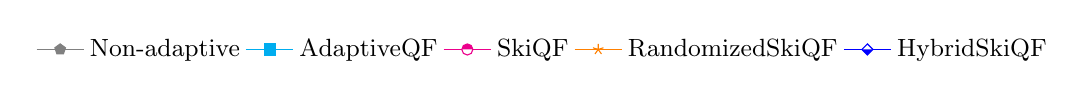
\begin{tikzpicture}
\begin{axis}[hide axis,xmin=0,xmax=1,ymin=0,ymax=1,
scale only axis,width=1cm,height=0.4cm,
legend columns=5,legend cell align=left,
legend style={draw=none,font=\small,at={(0.5,0.5)},anchor=center}]
\addlegendimage{skiqfNonAdaptive}
\addlegendentry{Non-adaptive}
\addlegendimage{skiqfAdaptive}
\addlegendentry{AdaptiveQF}
\addlegendimage{skiqfSki}
\addlegendentry{SkiQF}
\addlegendimage{skiqfRandomized}
\addlegendentry{RandomizedSkiQF}
\addlegendimage{skiqfHybrid}
\addlegendentry{HybridSkiQF}
\end{axis}\end{tikzpicture}
\par\medskip
\begingroup
\pgfmathsetlengthmacro{\skiqfpanelwidth}{(\linewidth-1.6cm-1.3cm)/2}
\begin{tikzpicture}\begin{groupplot}[skiqf axis,
group style={group size=2 by 1,horizontal sep=1.3cm,vertical sep=1.5cm},
scale only axis,width=\skiqfpanelwidth,height=3cm,scaled y ticks=true]
\nextgroupplot[title={Query throughput},
ylabel={Throughput\\(MOps/sec)},
ymin=0,
xlabel={Queries (millions)},
xmin=0,xmax=30,enlarge x limits=false]
\addplot[skiqfNonAdaptive,mark size=1.8pt,mark repeat=11] coordinates {(0.3,2.267813) (0.6,1.294998) (0.9,0.242336) (1.2,0.182133) (1.5,0.169625) (1.8,0.153999) (2.1,0.163409) (2.4,0.164695) (2.7,0.156378) (3,0.154179) (3.3,0.155929) (3.6,0.160073) (3.9,0.16026) (4.2,0.145551) (4.5,0.153359) (4.8,0.151729) (5.1,0.158269) (5.4,0.159324) (5.7,0.158171) (6,0.159554) (6.3,0.159365) (6.6,0.149043) (6.9,0.150055) (7.2,0.158589) (7.5,0.150635) (7.8,0.157284) (8.1,0.158228) (8.4,0.158495) (8.7,0.157245) (9,0.155257) (9.3,0.158869) (9.6,0.153805) (9.9,0.158175) (10.2,0.157269) (10.5,0.158855) (10.8,0.157537) (11.1,0.153127) (11.4,0.154901) (11.7,0.152635) (12,0.158448) (12.3,0.153969) (12.6,0.159374) (12.9,0.157908) (13.2,0.15883) (13.5,0.153457) (13.8,0.15761) (14.1,0.157223) (14.4,0.144833) (14.7,0.15397) (15,0.145075) (15.3,0.15886) (15.6,0.158004) (15.9,0.153565) (16.2,0.151886) (16.5,0.152978) (16.8,0.152293) (17.1,0.155533) (17.4,0.144199) (17.7,0.149341) (18,0.156681) (18.3,0.158541) (18.6,0.14356) (18.9,0.155493) (19.2,0.152714) (19.5,0.159158) (19.8,0.155214) (20.1,0.147917) (20.4,0.146139) (20.7,0.151914) (21,0.157948) (21.3,0.157689) (21.6,0.15589) (21.9,0.15363) (22.2,0.148144) (22.5,0.155491) (22.8,0.15805) (23.1,0.155252) (23.4,0.159318) (23.7,0.155814) (24,0.157162) (24.3,0.158758) (24.6,0.15873) (24.9,0.157044) (25.2,0.158175) (25.5,0.157984) (25.8,0.139142) (26.1,0.14748) (26.4,0.156028) (26.7,0.15601) (27,0.159315) (27.3,0.152966) (27.6,0.140472) (27.9,0.151944) (28.2,0.152025) (28.5,0.148109) (28.8,0.15549) (29.1,0.156816) (29.4,0.157091) (29.7,0.14883) (30,0.152347)};
\addplot[skiqfAdaptive,mark size=1.8pt,mark repeat=11] coordinates {(0.3,1.496024) (0.6,1.492628) (0.9,1.168762) (1.2,1.188694) (1.5,1.208876) (1.8,1.188937) (2.1,1.235646) (2.4,1.121101) (2.7,1.218548) (3,1.181203) (3.3,1.163277) (3.6,1.208314) (3.9,1.134832) (4.2,1.232533) (4.5,1.180986) (4.8,1.203846) (5.1,1.191463) (5.4,1.285584) (5.7,1.257784) (6,1.209892) (6.3,1.211491) (6.6,1.269424) (6.9,1.139265) (7.2,1.1542) (7.5,1.143065) (7.8,1.240424) (8.1,1.202623) (8.4,1.164653) (8.7,1.190646) (9,1.131863) (9.3,1.17502) (9.6,1.207702) (9.9,1.242283) (10.2,1.1825) (10.5,1.221097) (10.8,1.198051) (11.1,1.211457) (11.4,1.234923) (11.7,1.162985) (12,1.260565) (12.3,1.20434) (12.6,1.219979) (12.9,1.21346) (13.2,1.063717) (13.5,1.100494) (13.8,1.22246) (14.1,1.178687) (14.4,1.219245) (14.7,1.12541) (15,1.095941) (15.3,1.140017) (15.6,1.236963) (15.9,1.177266) (16.2,1.233073) (16.5,1.186509) (16.8,1.129067) (17.1,1.169087) (17.4,1.189938) (17.7,1.193955) (18,1.244467) (18.3,1.248995) (18.6,1.271568) (18.9,1.188338) (19.2,1.173523) (19.5,1.175734) (19.8,1.183125) (20.1,1.227475) (20.4,1.239111) (20.7,1.178644) (21,1.193273) (21.3,1.201978) (21.6,1.209272) (21.9,1.112972) (22.2,1.155843) (22.5,1.190854) (22.8,1.101011) (23.1,1.20569) (23.4,1.164038) (23.7,1.131876) (24,1.167892) (24.3,1.156525) (24.6,1.199432) (24.9,1.218834) (25.2,1.276136) (25.5,1.225093) (25.8,1.179635) (26.1,1.176874) (26.4,1.228283) (26.7,1.269194) (27,1.208289) (27.3,1.037395) (27.6,1.11555) (27.9,1.209247) (28.2,1.173965) (28.5,1.137982) (28.8,1.116024) (29.1,1.169329) (29.4,1.168492) (29.7,1.1874) (30,1.229303)};
\addplot[skiqfSki,mark size=1.8pt,mark repeat=11] coordinates {(0.3,1.422819) (0.6,1.450846) (0.9,1.12663) (1.2,1.060444) (1.5,1.029361) (1.8,1.048767) (2.1,1.02568) (2.4,0.974604) (2.7,0.938418) (3,0.822231) (3.3,1.05823) (3.6,1.099957) (3.9,1.051691) (4.2,0.911167) (4.5,0.790829) (4.8,1.082969) (5.1,1.108314) (5.4,1.188216) (5.7,1.142892) (6,0.984354) (6.3,0.8269) (6.6,0.855843) (6.9,0.836912) (7.2,0.812267) (7.5,0.814397) (7.8,0.841289) (8.1,0.830866) (8.4,0.800622) (8.7,0.83839) (9,0.761568) (9.3,0.811207) (9.6,0.82065) (9.9,0.827281) (10.2,0.797966) (10.5,0.821419) (10.8,0.795318) (11.1,0.824113) (11.4,0.84579) (11.7,0.801507) (12,0.840375) (12.3,0.852197) (12.6,0.839561) (12.9,0.83034) (13.2,0.84725) (13.5,0.769027) (13.8,0.829259) (14.1,0.794377) (14.4,0.824276) (14.7,0.826586) (15,0.783268) (15.3,0.793867) (15.6,0.794272) (15.9,0.793011) (16.2,0.847094) (16.5,0.822432) (16.8,0.814251) (17.1,0.79531) (17.4,0.807099) (17.7,0.830096) (18,0.829717) (18.3,0.879797) (18.6,0.857426) (18.9,0.834869) (19.2,0.842819) (19.5,0.835724) (19.8,0.829498) (20.1,0.857663) (20.4,0.828555) (20.7,0.823233) (21,0.79952) (21.3,0.813413) (21.6,0.807127) (21.9,0.801246) (22.2,0.778754) (22.5,0.802022) (22.8,0.827395) (23.1,0.838576) (23.4,0.807444) (23.7,0.788216) (24,0.776493) (24.3,0.79668) (24.6,0.747679) (24.9,0.827185) (25.2,0.843653) (25.5,0.871608) (25.8,0.83076) (26.1,0.806858) (26.4,0.869649) (26.7,0.867014) (27,0.832349) (27.3,0.808583) (27.6,0.838892) (27.9,0.822216) (28.2,0.809193) (28.5,0.838471) (28.8,0.80159) (29.1,0.793097) (29.4,0.807341) (29.7,0.784767) (30,0.852127)};
\addplot[skiqfRandomized,mark size=1.8pt,mark repeat=11] coordinates {(0.3,1.485122) (0.6,1.457063) (0.9,1.038728) (1.2,1.084998) (1.5,1.09968) (1.8,1.010333) (2.1,1.048231) (2.4,0.935779) (2.7,0.811393) (3,0.959209) (3.3,0.927804) (3.6,0.906751) (3.9,1.154353) (4.2,1.130977) (4.5,0.903506) (4.8,1.069595) (5.1,1.008936) (5.4,1.231945) (5.7,1.114196) (6,1.208675) (6.3,1.175738) (6.6,1.271393) (6.9,1.142276) (7.2,1.110218) (7.5,0.962633) (7.8,1.046365) (8.1,0.948616) (8.4,0.874808) (8.7,0.921975) (9,0.889783) (9.3,0.93202) (9.6,0.933692) (9.9,0.91517) (10.2,0.907981) (10.5,0.89212) (10.8,0.818287) (11.1,0.90741) (11.4,0.795858) (11.7,0.891332) (12,0.978383) (12.3,0.927001) (12.6,0.785269) (12.9,0.898561) (13.2,0.845758) (13.5,0.819693) (13.8,0.972202) (14.1,0.904055) (14.4,0.899011) (14.7,0.903108) (15,0.861235) (15.3,0.922596) (15.6,0.961547) (15.9,0.895916) (16.2,0.941685) (16.5,0.873762) (16.8,0.779056) (17.1,0.850581) (17.4,0.89132) (17.7,0.948071) (18,0.910713) (18.3,0.939553) (18.6,0.953091) (18.9,0.95778) (19.2,0.914232) (19.5,0.823977) (19.8,0.895018) (20.1,1.013525) (20.4,0.92411) (20.7,0.931585) (21,0.921174) (21.3,0.957862) (21.6,0.939244) (21.9,0.895339) (22.2,0.918987) (22.5,0.891117) (22.8,0.907179) (23.1,0.893064) (23.4,0.84098) (23.7,0.815461) (24,0.824115) (24.3,0.861468) (24.6,0.898069) (24.9,0.960382) (25.2,0.982717) (25.5,0.977914) (25.8,0.924852) (26.1,0.949593) (26.4,0.914445) (26.7,0.948176) (27,0.867931) (27.3,0.898195) (27.6,0.989273) (27.9,0.868607) (28.2,0.932068) (28.5,0.878789) (28.8,0.916118) (29.1,0.928) (29.4,0.864432) (29.7,0.813068) (30,0.913589)};
\addplot[skiqfHybrid,mark size=1.8pt,mark repeat=11] coordinates {(0.3,1.62487) (0.6,1.588016) (0.9,1.386533) (1.2,1.199087) (1.5,1.264766) (1.8,1.081617) (2.1,1.195277) (2.4,1.245433) (2.7,1.28008) (3,1.106494) (3.3,1.17854) (3.6,1.183653) (3.9,1.207386) (4.2,1.221176) (4.5,1.186495) (4.8,1.256934) (5.1,1.202334) (5.4,1.272883) (5.7,1.292485) (6,1.240641) (6.3,1.208066) (6.6,0.905459) (6.9,1.217538) (7.2,1.18487) (7.5,0.849485) (7.8,1.240727) (8.1,0.451944) (8.4,1.217549) (8.7,1.249403) (9,0.427054) (9.3,1.183674) (9.6,0.430857) (9.9,1.220266) (10.2,0.408869) (10.5,1.203991) (10.8,0.40428) (11.1,1.20178) (11.4,0.405958) (11.7,1.174463) (12,0.401808) (12.3,1.214633) (12.6,0.401734) (12.9,1.252196) (13.2,1.244587) (13.5,0.388623) (13.8,1.261268) (14.1,0.376193) (14.4,1.196825) (14.7,0.240631) (15,0.242461) (15.3,0.404719) (15.6,0.229217) (15.9,0.226683) (16.2,0.210324) (16.5,0.221981) (16.8,0.220903) (17.1,0.382534) (17.4,0.380884) (17.7,0.352684) (18,0.216873) (18.3,0.375266) (18.6,0.354991) (18.9,0.156116) (19.2,0.366308) (19.5,0.225866) (19.8,0.214117) (20.1,0.221731) (20.4,0.212247) (20.7,0.226598) (21,0.161253) (21.3,0.228218) (21.6,1.202214) (21.9,0.374225) (22.2,0.37287) (22.5,0.373635) (22.8,0.22478) (23.1,0.375215) (23.4,0.225976) (23.7,0.379237) (24,0.356222) (24.3,0.356786) (24.6,0.342803) (24.9,0.378388) (25.2,0.353547) (25.5,0.366913) (25.8,0.222242) (26.1,0.374622) (26.4,0.160132) (26.7,0.373934) (27,0.217497) (27.3,0.2185) (27.6,0.228012) (27.9,0.218683) (28.2,0.144052) (28.5,0.381853) (28.8,0.154848) (29.1,0.218691) (29.4,0.372963) (29.7,0.225034) (30,0.219674)};
\nextgroupplot[title={False positives},
ylabel={False positive rate},
ymin=0,
xlabel={Queries (millions)},
xmin=0,xmax=30,enlarge x limits=false]
\addplot[skiqfNonAdaptive,mark size=1.8pt,mark repeat=11] coordinates {(0.3,0.05315333333) (0.6,0.05348) (0.9,0.05336) (1.2,0.05343666667) (1.5,0.05333666667) (1.8,0.05340333333) (2.1,0.05334333333) (2.4,0.05322333333) (2.7,0.05325) (3,0.05333333333) (3.3,0.05347) (3.6,0.05345666667) (3.9,0.0532) (4.2,0.05335) (4.5,0.05340333333) (4.8,0.05335666667) (5.1,0.05325) (5.4,0.05339) (5.7,0.05307) (6,0.05314666667) (6.3,0.05327) (6.6,0.05322333333) (6.9,0.05316333333) (7.2,0.05338) (7.5,0.05339666667) (7.8,0.05334333333) (8.1,0.05331666667) (8.4,0.05326666667) (8.7,0.05337666667) (9,0.0533) (9.3,0.05337) (9.6,0.05348333333) (9.9,0.05325) (10.2,0.05326333333) (10.5,0.05336333333) (10.8,0.05337) (11.1,0.05322) (11.4,0.05343333333) (11.7,0.05335666667) (12,0.05321666667) (12.3,0.05334) (12.6,0.05318333333) (12.9,0.05322) (13.2,0.05329) (13.5,0.05331333333) (13.8,0.05329666667) (14.1,0.05333333333) (14.4,0.05323) (14.7,0.05322) (15,0.05349666667) (15.3,0.05330666667) (15.6,0.05332666667) (15.9,0.05342) (16.2,0.05342666667) (16.5,0.05331) (16.8,0.05338666667) (17.1,0.05322666667) (17.4,0.05338) (17.7,0.05347) (18,0.05340666667) (18.3,0.05338666667) (18.6,0.05334333333) (18.9,0.05328) (19.2,0.05320666667) (19.5,0.05315333333) (19.8,0.05335) (20.1,0.05323333333) (20.4,0.05328333333) (20.7,0.05343333333) (21,0.05316333333) (21.3,0.05331) (21.6,0.05325666667) (21.9,0.05342333333) (22.2,0.05331666667) (22.5,0.05333) (22.8,0.0534) (23.1,0.05349) (23.4,0.05340333333) (23.7,0.05344666667) (24,0.05333) (24.3,0.05328) (24.6,0.05342666667) (24.9,0.05359666667) (25.2,0.05349333333) (25.5,0.05353666667) (25.8,0.05343666667) (26.1,0.05324333333) (26.4,0.05323666667) (26.7,0.05327666667) (27,0.05322333333) (27.3,0.05346333333) (27.6,0.05315333333) (27.9,0.05323333333) (28.2,0.05328) (28.5,0.05325333333) (28.8,0.05338333333) (29.1,0.05341) (29.4,0.05330666667) (29.7,0.05340333333) (30,0.05338333333)};
\addplot[skiqfAdaptive,mark size=1.8pt,mark repeat=11] coordinates {(0.3,0.003313333333) (0.6,0.003733333333) (0.9,0.003506666667) (1.2,0.003543333333) (1.5,0.00355) (1.8,0.0036) (2.1,0.003403333333) (2.4,0.003466666667) (2.7,0.00337) (3,0.003643333333) (3.3,0.00367) (3.6,0.003426666667) (3.9,0.003566666667) (4.2,0.003446666667) (4.5,0.00359) (4.8,0.003446666667) (5.1,0.00353) (5.4,0.003273333333) (5.7,0.003293333333) (6,0.00344) (6.3,0.003413333333) (6.6,0.003323333333) (6.9,0.0035) (7.2,0.003563333333) (7.5,0.003596666667) (7.8,0.003376666667) (8.1,0.003453333333) (8.4,0.003623333333) (8.7,0.003493333333) (9,0.003646666667) (9.3,0.003493333333) (9.6,0.003423333333) (9.9,0.003386666667) (10.2,0.003543333333) (10.5,0.003496666667) (10.8,0.003543333333) (11.1,0.003533333333) (11.4,0.003393333333) (11.7,0.00349) (12,0.003326666667) (12.3,0.0034) (12.6,0.003423333333) (12.9,0.00351) (13.2,0.003426666667) (13.5,0.0036) (13.8,0.003273333333) (14.1,0.003636666667) (14.4,0.00338) (14.7,0.003493333333) (15,0.00375) (15.3,0.003546666667) (15.6,0.003416666667) (15.9,0.003603333333) (16.2,0.00339) (16.5,0.003526666667) (16.8,0.003623333333) (17.1,0.00355) (17.4,0.00354) (17.7,0.003526666667) (18,0.003356666667) (18.3,0.00342) (18.6,0.003296666667) (18.9,0.003463333333) (19.2,0.003403333333) (19.5,0.003593333333) (19.8,0.00339) (20.1,0.00341) (20.4,0.0034) (20.7,0.00355) (21,0.00352) (21.3,0.003456666667) (21.6,0.003476666667) (21.9,0.003726666667) (22.2,0.003606666667) (22.5,0.00353) (22.8,0.003516666667) (23.1,0.00347) (23.4,0.003593333333) (23.7,0.003743333333) (24,0.00363) (24.3,0.00367) (24.6,0.00353) (24.9,0.003483333333) (25.2,0.003313333333) (25.5,0.00339) (25.8,0.003513333333) (26.1,0.003436666667) (26.4,0.003423333333) (26.7,0.0033) (27,0.003496666667) (27.3,0.003556666667) (27.6,0.003463333333) (27.9,0.00351) (28.2,0.003553333333) (28.5,0.003556666667) (28.8,0.003546666667) (29.1,0.00354) (29.4,0.003573333333) (29.7,0.003546666667) (30,0.003413333333)};
\addplot[skiqfSki,mark size=1.8pt,mark repeat=11] coordinates {(0.3,0.006493333333) (0.6,0.00731) (0.9,0.006813333333) (1.2,0.007036666667) (1.5,0.006966666667) (1.8,0.006936666667) (2.1,0.006743333333) (2.4,0.006783333333) (2.7,0.006626666667) (3,0.007086666667) (3.3,0.007193333333) (3.6,0.006763333333) (3.9,0.00697) (4.2,0.00679) (4.5,0.007073333333) (4.8,0.00671) (5.1,0.006926666667) (5.4,0.00646) (5.7,0.00646) (6,0.006716666667) (6.3,0.00674) (6.6,0.006503333333) (6.9,0.006893333333) (7.2,0.007006666667) (7.5,0.006933333333) (7.8,0.006726666667) (8.1,0.006723333333) (8.4,0.007016666667) (8.7,0.00673) (9,0.00734) (9.3,0.006893333333) (9.6,0.00661) (9.9,0.006733333333) (10.2,0.007023333333) (10.5,0.006743333333) (10.8,0.007013333333) (11.1,0.00682) (11.4,0.006636666667) (11.7,0.00705) (12,0.006503333333) (12.3,0.00664) (12.6,0.006786666667) (12.9,0.00685) (13.2,0.006733333333) (13.5,0.006966666667) (13.8,0.006416666667) (14.1,0.007093333333) (14.4,0.006803333333) (14.7,0.00678) (15,0.007106666667) (15.3,0.00709) (15.6,0.006703333333) (15.9,0.006956666667) (16.2,0.006746666667) (16.5,0.006956666667) (16.8,0.006956666667) (17.1,0.00706) (17.4,0.007036666667) (17.7,0.006773333333) (18,0.00688) (18.3,0.00645) (18.6,0.006596666667) (18.9,0.006723333333) (19.2,0.00672) (19.5,0.0069) (19.8,0.006763333333) (20.1,0.00652) (20.4,0.006826666667) (20.7,0.006926666667) (21,0.006783333333) (21.3,0.006893333333) (21.6,0.00686) (21.9,0.007106666667) (22.2,0.007106666667) (22.5,0.007126666667) (22.8,0.006776666667) (23.1,0.006746666667) (23.4,0.007073333333) (23.7,0.00722) (24,0.00728) (24.3,0.007156666667) (24.6,0.007073333333) (24.9,0.006826666667) (25.2,0.006566666667) (25.5,0.006556666667) (25.8,0.006753333333) (26.1,0.006923333333) (26.4,0.006553333333) (26.7,0.00658) (27,0.006686666667) (27.3,0.006936666667) (27.6,0.006786666667) (27.9,0.006853333333) (28.2,0.00704) (28.5,0.006833333333) (28.8,0.006986666667) (29.1,0.00704) (29.4,0.007013333333) (29.7,0.007076666667) (30,0.006616666667)};
\addplot[skiqfRandomized,mark size=1.8pt,mark repeat=11] coordinates {(0.3,0.00548) (0.6,0.00618) (0.9,0.005663333333) (1.2,0.00579) (1.5,0.00594) (1.8,0.005936666667) (2.1,0.005706666667) (2.4,0.005656666667) (2.7,0.005713333333) (3,0.006016666667) (3.3,0.006093333333) (3.6,0.00566) (3.9,0.005906666667) (4.2,0.005843333333) (4.5,0.005923333333) (4.8,0.005566666667) (5.1,0.00579) (5.4,0.005456666667) (5.7,0.00537) (6,0.005593333333) (6.3,0.00569) (6.6,0.005493333333) (6.9,0.005796666667) (7.2,0.00581) (7.5,0.005886666667) (7.8,0.005496666667) (8.1,0.005586666667) (8.4,0.005856666667) (8.7,0.005766666667) (9,0.006053333333) (9.3,0.005703333333) (9.6,0.00556) (9.9,0.005516666667) (10.2,0.00592) (10.5,0.005626666667) (10.8,0.00578) (11.1,0.005763333333) (11.4,0.0056) (11.7,0.005906666667) (12,0.005376666667) (12.3,0.00554) (12.6,0.005713333333) (12.9,0.005583333333) (13.2,0.00565) (13.5,0.00613) (13.8,0.00532) (14.1,0.005903333333) (14.4,0.005666666667) (14.7,0.00571) (15,0.006066666667) (15.3,0.005923333333) (15.6,0.005473333333) (15.9,0.005936666667) (16.2,0.005576666667) (16.5,0.006023333333) (16.8,0.005876666667) (17.1,0.005763333333) (17.4,0.005876666667) (17.7,0.00569) (18,0.00577) (18.3,0.005643333333) (18.6,0.005353333333) (18.9,0.005633333333) (19.2,0.005606666667) (19.5,0.005863333333) (19.8,0.005733333333) (20.1,0.005393333333) (20.4,0.005753333333) (20.7,0.005786666667) (21,0.005636666667) (21.3,0.005683333333) (21.6,0.005713333333) (21.9,0.00603) (22.2,0.00594) (22.5,0.00596) (22.8,0.00576) (23.1,0.005626666667) (23.4,0.00588) (23.7,0.006056666667) (24,0.00587) (24.3,0.00612) (24.6,0.00583) (24.9,0.005766666667) (25.2,0.005576666667) (25.5,0.00541) (25.8,0.005713333333) (26.1,0.005736666667) (26.4,0.005626666667) (26.7,0.005543333333) (27,0.005616666667) (27.3,0.00586) (27.6,0.0055) (27.9,0.005953333333) (28.2,0.00587) (28.5,0.005763333333) (28.8,0.005873333333) (29.1,0.005883333333) (29.4,0.00584) (29.7,0.005896666667) (30,0.00547)};
\addplot[skiqfHybrid,mark size=1.8pt,mark repeat=11] coordinates {(0.3,0.01993333333) (0.6,0.003716666667) (0.9,0.02009666667) (1.2,0.003563333333) (1.5,0.02015333333) (1.8,0.003533333333) (2.1,0.003453333333) (2.4,0.003476666667) (2.7,0.00335) (3,0.00363) (3.3,0.00369) (3.6,0.00343) (3.9,0.00355) (4.2,0.003463333333) (4.5,0.003616666667) (4.8,0.003413333333) (5.1,0.003536666667) (5.4,0.0033) (5.7,0.003283333333) (6,0.00342) (6.3,0.003463333333) (6.6,0.01985333333) (6.9,0.003533333333) (7.2,0.00359) (7.5,0.02005333333) (7.8,0.003426666667) (8.1,0.01997666667) (8.4,0.00356) (8.7,0.003446666667) (9,0.02034666667) (9.3,0.00351) (9.6,0.01994666667) (9.9,0.00345) (10.2,0.02013333333) (10.5,0.003523333333) (10.8,0.02014666667) (11.1,0.003473333333) (11.4,0.01994) (11.7,0.00363) (12,0.01987333333) (12.3,0.003406666667) (12.6,0.02004333333) (12.9,0.003446666667) (13.2,0.003416666667) (13.5,0.02014666667) (13.8,0.003293333333) (14.1,0.02016) (14.4,0.00352) (14.7,0.03668666667) (15,0.03664) (15.3,0.02015333333) (15.6,0.03669666667) (15.9,0.03671333333) (16.2,0.03665) (16.5,0.03669666667) (16.8,0.03678) (17.1,0.02006333333) (17.4,0.02014333333) (17.7,0.01995) (18,0.03667333333) (18.3,0.01985333333) (18.6,0.01992333333) (18.9,0.05333666667) (19.2,0.02011) (19.5,0.03658) (19.8,0.03671333333) (20.1,0.03649) (20.4,0.03668666667) (20.7,0.03651) (21,0.05335666667) (21.3,0.03669) (21.6,0.003463333333) (21.9,0.01996666667) (22.2,0.02022666667) (22.5,0.02020666667) (22.8,0.03674) (23.1,0.02012) (23.4,0.03661) (23.7,0.02021333333) (24,0.02036) (24.3,0.02012) (24.6,0.02033) (24.9,0.02009333333) (25.2,0.01992333333) (25.5,0.01994333333) (25.8,0.03656) (26.1,0.02009333333) (26.4,0.05325) (26.7,0.01991) (27,0.03650333333) (27.3,0.03666333333) (27.6,0.03667) (27.9,0.03674666667) (28.2,0.05319) (28.5,0.02000333333) (28.8,0.05327333333) (29.1,0.03675333333) (29.4,0.02027) (29.7,0.03666) (30,0.0369)};
\end{groupplot}\end{tikzpicture}\endgroup\end{center}

\begin{center}\small Perfect recognition of ordinary query outcomes: corrections immediately disable replay; tolerated false positives enable it. There are no probes or adversary windows. HybridSkiQF's detector window is 100,000 negative-key queries; smoothing remains 0.7 and the repeated-FP threshold remains 6.\end{center}
\begin{center}
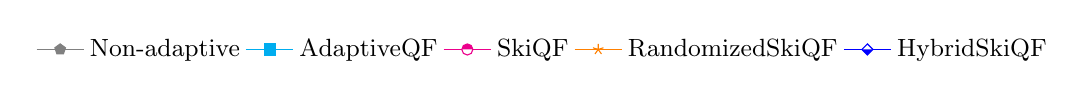
\begin{tikzpicture}
\begin{axis}[hide axis,xmin=0,xmax=1,ymin=0,ymax=1,
scale only axis,width=1cm,height=0.4cm,
legend columns=5,legend cell align=left,
legend style={draw=none,font=\small,at={(0.5,0.5)},anchor=center}]
\addlegendimage{skiqfNonAdaptive}
\addlegendentry{Non-adaptive}
\addlegendimage{skiqfAdaptive}
\addlegendentry{AdaptiveQF}
\addlegendimage{skiqfSki}
\addlegendentry{SkiQF}
\addlegendimage{skiqfRandomized}
\addlegendentry{RandomizedSkiQF}
\addlegendimage{skiqfHybrid}
\addlegendentry{HybridSkiQF}
\end{axis}\end{tikzpicture}
\par\medskip
\begingroup
\pgfmathsetlengthmacro{\skiqfpanelwidth}{(\linewidth-1.6cm-0.0cm)/1}
\begin{tikzpicture}\begin{groupplot}[skiqf axis,
group style={group size=1 by 1,horizontal sep=0.7cm,vertical sep=1.5cm},
scale only axis,width=\skiqfpanelwidth,height=3cm,scaled y ticks=true]
\nextgroupplot[title={Replay flag},
ylabel={Fraction of queries\\with replay enabled},
ymin=0,
xlabel={Queries (millions)},
xmin=0,xmax=30,enlarge x limits=false]
\addplot[skiqfNonAdaptive,mark size=1.8pt,mark repeat=11] coordinates {(0.3,0.9999566667) (0.6,1) (0.9,1) (1.2,1) (1.5,1) (1.8,1) (2.1,1) (2.4,1) (2.7,1) (3,1) (3.3,1) (3.6,1) (3.9,1) (4.2,1) (4.5,1) (4.8,1) (5.1,1) (5.4,1) (5.7,1) (6,1) (6.3,1) (6.6,1) (6.9,1) (7.2,1) (7.5,1) (7.8,1) (8.1,1) (8.4,1) (8.7,1) (9,1) (9.3,1) (9.6,1) (9.9,1) (10.2,1) (10.5,1) (10.8,1) (11.1,1) (11.4,1) (11.7,1) (12,1) (12.3,1) (12.6,1) (12.9,1) (13.2,1) (13.5,1) (13.8,1) (14.1,1) (14.4,1) (14.7,1) (15,1) (15.3,1) (15.6,1) (15.9,1) (16.2,1) (16.5,1) (16.8,1) (17.1,1) (17.4,1) (17.7,1) (18,1) (18.3,1) (18.6,1) (18.9,1) (19.2,1) (19.5,1) (19.8,1) (20.1,1) (20.4,1) (20.7,1) (21,1) (21.3,1) (21.6,1) (21.9,1) (22.2,1) (22.5,1) (22.8,1) (23.1,1) (23.4,1) (23.7,1) (24,1) (24.3,1) (24.6,1) (24.9,1) (25.2,1) (25.5,1) (25.8,1) (26.1,1) (26.4,1) (26.7,1) (27,1) (27.3,1) (27.6,1) (27.9,1) (28.2,1) (28.5,1) (28.8,1) (29.1,1) (29.4,1) (29.7,1) (30,1)};
\addplot[skiqfAdaptive,mark size=1.8pt,mark repeat=11] coordinates {(0.3,0) (0.6,0) (0.9,0) (1.2,0) (1.5,0) (1.8,0) (2.1,0) (2.4,0) (2.7,0) (3,0) (3.3,0) (3.6,0) (3.9,0) (4.2,0) (4.5,0) (4.8,0) (5.1,0) (5.4,0) (5.7,0) (6,0) (6.3,0) (6.6,0) (6.9,0) (7.2,0) (7.5,0) (7.8,0) (8.1,0) (8.4,0) (8.7,0) (9,0) (9.3,0) (9.6,0) (9.9,0) (10.2,0) (10.5,0) (10.8,0) (11.1,0) (11.4,0) (11.7,0) (12,0) (12.3,0) (12.6,0) (12.9,0) (13.2,0) (13.5,0) (13.8,0) (14.1,0) (14.4,0) (14.7,0) (15,0) (15.3,0) (15.6,0) (15.9,0) (16.2,0) (16.5,0) (16.8,0) (17.1,0) (17.4,0) (17.7,0) (18,0) (18.3,0) (18.6,0) (18.9,0) (19.2,0) (19.5,0) (19.8,0) (20.1,0) (20.4,0) (20.7,0) (21,0) (21.3,0) (21.6,0) (21.9,0) (22.2,0) (22.5,0) (22.8,0) (23.1,0) (23.4,0) (23.7,0) (24,0) (24.3,0) (24.6,0) (24.9,0) (25.2,0) (25.5,0) (25.8,0) (26.1,0) (26.4,0) (26.7,0) (27,0) (27.3,0) (27.6,0) (27.9,0) (28.2,0) (28.5,0) (28.8,0) (29.1,0) (29.4,0) (29.7,0) (30,0)};
\addplot[skiqfSki,mark size=1.8pt,mark repeat=11] coordinates {(0.3,0.03385666667) (0.6,0.03917) (0.9,0.03609666667) (1.2,0.03664666667) (1.5,0.03645) (1.8,0.03644666667) (2.1,0.03479666667) (2.4,0.03500333333) (2.7,0.03535333333) (3,0.03565333333) (3.3,0.03702333333) (3.6,0.03398333333) (3.9,0.03578666667) (4.2,0.03552) (4.5,0.03704) (4.8,0.03531666667) (5.1,0.03587) (5.4,0.03333666667) (5.7,0.03357333333) (6,0.03549666667) (6.3,0.03609333333) (6.6,0.03423666667) (6.9,0.03581333333) (7.2,0.03653666667) (7.5,0.03494666667) (7.8,0.03587333333) (8.1,0.03456) (8.4,0.03758333333) (8.7,0.03366333333) (9,0.03933) (9.3,0.03547) (9.6,0.03402666667) (9.9,0.03494) (10.2,0.03665333333) (10.5,0.03511) (10.8,0.03649666667) (11.1,0.03502) (11.4,0.03506666667) (11.7,0.03712333333) (12,0.03397666667) (12.3,0.03429666667) (12.6,0.03537666667) (12.9,0.03700333333) (13.2,0.03337333333) (13.5,0.03578) (13.8,0.03345333333) (14.1,0.03772333333) (14.4,0.03534) (14.7,0.03453) (15,0.03694) (15.3,0.03753) (15.6,0.03541) (15.9,0.03616333333) (16.2,0.03558666667) (16.5,0.03538) (16.8,0.03556333333) (17.1,0.03662333333) (17.4,0.03632333333) (17.7,0.03435333333) (18,0.03521) (18.3,0.0335) (18.6,0.03398666667) (18.9,0.03472666667) (19.2,0.03495) (19.5,0.03524) (19.8,0.03531666667) (20.1,0.03480333333) (20.4,0.03543) (20.7,0.03544) (21,0.0361) (21.3,0.03663666667) (21.6,0.03535333333) (21.9,0.03713) (22.2,0.03749) (22.5,0.03491333333) (22.8,0.03529666667) (23.1,0.03509) (23.4,0.03697333333) (23.7,0.03694666667) (24,0.03844666667) (24.3,0.03733333333) (24.6,0.03695) (24.9,0.03537666667) (25.2,0.03500666667) (25.5,0.03362666667) (25.8,0.03470333333) (26.1,0.03669) (26.4,0.03386) (26.7,0.03427) (27,0.03354333333) (27.3,0.03685666667) (27.6,0.03492666667) (27.9,0.03664666667) (28.2,0.03661333333) (28.5,0.03435) (28.8,0.03716) (29.1,0.03573333333) (29.4,0.03586333333) (29.7,0.03662) (30,0.03458333333)};
\addplot[skiqfRandomized,mark size=1.8pt,mark repeat=11] coordinates {(0.3,0.02195) (0.6,0.02601) (0.9,0.02331666667) (1.2,0.02326666667) (1.5,0.02649) (1.8,0.02515) (2.1,0.02426333333) (2.4,0.02322666667) (2.7,0.02398333333) (3,0.02565) (3.3,0.0258) (3.6,0.02446666667) (3.9,0.02479333333) (4.2,0.02430333333) (4.5,0.02467333333) (4.8,0.02310333333) (5.1,0.02400333333) (5.4,0.02319333333) (5.7,0.02173) (6,0.02263333333) (6.3,0.02384333333) (6.6,0.02319) (6.9,0.02396) (7.2,0.02327333333) (7.5,0.02533666667) (7.8,0.02210666667) (8.1,0.02399666667) (8.4,0.02384666667) (8.7,0.02469333333) (9,0.02491666667) (9.3,0.02357666667) (9.6,0.02306666667) (9.9,0.02238) (10.2,0.02575) (10.5,0.02328) (10.8,0.02376) (11.1,0.02369) (11.4,0.02220333333) (11.7,0.02507666667) (12,0.02234) (12.3,0.02211666667) (12.6,0.02359) (12.9,0.02327666667) (13.2,0.02350333333) (13.5,0.02676) (13.8,0.02149666667) (14.1,0.02373666667) (14.4,0.02380333333) (14.7,0.02401) (15,0.02506666667) (15.3,0.02371333333) (15.6,0.02233) (15.9,0.02524333333) (16.2,0.02346) (16.5,0.02488666667) (16.8,0.02450666667) (17.1,0.02351) (17.4,0.02436333333) (17.7,0.02367333333) (18,0.02476666667) (18.3,0.02437) (18.6,0.02228666667) (18.9,0.02428666667) (19.2,0.02343666667) (19.5,0.02409) (19.8,0.02298666667) (20.1,0.02239333333) (20.4,0.02396) (20.7,0.02438666667) (21,0.02365333333) (21.3,0.02405) (21.6,0.02317) (21.9,0.02435333333) (22.2,0.02554) (22.5,0.02500333333) (22.8,0.02442666667) (23.1,0.02471666667) (23.4,0.02522) (23.7,0.02376333333) (24,0.02384333333) (24.3,0.02638666667) (24.6,0.02429) (24.9,0.02436333333) (25.2,0.02365333333) (25.5,0.02214) (25.8,0.02446666667) (26.1,0.02424) (26.4,0.02242666667) (26.7,0.02372333333) (27,0.02260666667) (27.3,0.02359) (27.6,0.02127) (27.9,0.02546666667) (28.2,0.02570333333) (28.5,0.02353333333) (28.8,0.02507666667) (29.1,0.02442666667) (29.4,0.02484) (29.7,0.02471666667) (30,0.02222333333)};
\addplot[skiqfHybrid,mark size=1.8pt,mark repeat=11] coordinates {(0.3,0.3332933333) (0.6,0) (0.9,0.3329133333) (1.2,0) (1.5,0.33319) (1.8,3.333333333e-06) (2.1,0) (2.4,0) (2.7,0) (3,0) (3.3,0) (3.6,0) (3.9,0) (4.2,0) (4.5,0) (4.8,0) (5.1,0) (5.4,0) (5.7,0) (6,0) (6.3,0) (6.6,0.33316) (6.9,3.333333333e-06) (7.2,0) (7.5,0.3314133333) (7.8,0) (8.1,0.3315933333) (8.4,0) (8.7,0) (9,0.3331466667) (9.3,0) (9.6,0.33275) (9.9,3.333333333e-06) (10.2,0.33324) (10.5,3.333333333e-06) (10.8,0.3332066667) (11.1,3.333333333e-06) (11.4,0.3330966667) (11.7,3.333333333e-06) (12,0.3325133333) (12.3,3.333333333e-06) (12.6,0.33314) (12.9,3.333333333e-06) (13.2,0) (13.5,0.3326233333) (13.8,3.333333333e-06) (14.1,0.3329133333) (14.4,0) (14.7,0.6662833333) (15,0.66328) (15.3,0.3333366667) (15.6,0.6665266667) (15.9,0.6654633333) (16.2,0.6658333333) (16.5,0.6662633333) (16.8,0.66634) (17.1,0.33118) (17.4,0.3327933333) (17.7,0.32781) (18,0.66656) (18.3,0.3333366667) (18.6,0.33298) (18.9,1) (19.2,0.3327233333) (19.5,0.6665466667) (19.8,0.6659733333) (20.1,0.6643133333) (20.4,0.6664666667) (20.7,0.6643833333) (21,1) (21.3,0.6654866667) (21.6,3.333333333e-06) (21.9,0.3307033333) (22.2,0.3315733333) (22.5,0.3332333333) (22.8,0.6660866667) (23.1,0.33314) (23.4,0.6655133333) (23.7,0.33325) (24,0.3332866667) (24.3,0.3317433333) (24.6,0.3326033333) (24.9,0.3329433333) (25.2,0.3296066667) (25.5,0.33319) (25.8,0.6665966667) (26.1,0.3328033333) (26.4,0.9985966667) (26.7,0.33223) (27,0.6653233333) (27.3,0.66667) (27.6,0.6652866667) (27.9,0.66667) (28.2,0.99824) (28.5,0.3294266667) (28.8,0.9999) (29.1,0.6664533333) (29.4,0.33258) (29.7,0.6653366667) (30,0.6665066667)};
\end{groupplot}\end{tikzpicture}\endgroup\end{center}

\begin{center}\small The flag changes immediately; the plot averages its value over each reporting interval.\end{center}
\begin{center}
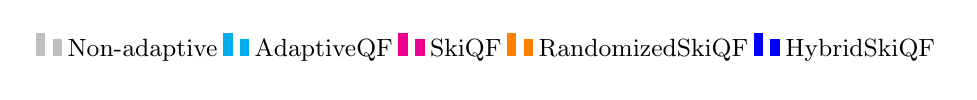
\begin{tikzpicture}
\begin{axis}[hide axis,xmin=0,xmax=1,ymin=0,ymax=1,
scale only axis,width=1cm,height=0.4cm,
legend columns=5,legend cell align=left,
legend style={draw=none,font=\small,at={(0.5,0.5)},anchor=center}]
\addlegendimage{ybar legend,/tikz/ybar,skiqfNonAdaptiveBar}
\addlegendentry{Non-adaptive}
\addlegendimage{ybar legend,/tikz/ybar,skiqfAdaptiveBar}
\addlegendentry{AdaptiveQF}
\addlegendimage{ybar legend,/tikz/ybar,skiqfSkiBar}
\addlegendentry{SkiQF}
\addlegendimage{ybar legend,/tikz/ybar,skiqfRandomizedBar}
\addlegendentry{RandomizedSkiQF}
\addlegendimage{ybar legend,/tikz/ybar,skiqfHybridBar}
\addlegendentry{HybridSkiQF}
\end{axis}\end{tikzpicture}
\par\medskip
\begingroup
\pgfmathsetlengthmacro{\skiqfpanelwidth}{(\linewidth-1.6cm-0.0cm)/1}
\begin{tikzpicture}\begin{groupplot}[skiqf axis,
group style={group size=1 by 1,horizontal sep=0.7cm,vertical sep=1.5cm},
scale only axis,width=\skiqfpanelwidth,height=3cm,scaled y ticks=true]
\nextgroupplot[title={Corrections by traffic regime},
ylabel={Corrections},
ymin=0,
ybar=0,bar width=5pt,enlarge x limits=false,
xmin=-0.5,xmax=1.5,
xtick={0,1},
xticklabels={Replay disabled,Replay enabled},
x tick label style={rotate=45,anchor=east,font=\scriptsize}]
\addplot[skiqfNonAdaptiveBar,mark size=1.8pt,mark repeat=1] coordinates {(0,0) (1,0)};
\addplot[skiqfAdaptiveBar,mark size=1.8pt,mark repeat=1] coordinates {(0,104826) (1,0)};
\addplot[skiqfSkiBar,mark size=1.8pt,mark repeat=1] coordinates {(0,8) (1,101043)};
\addplot[skiqfRandomizedBar,mark size=1.8pt,mark repeat=1] coordinates {(0,33876) (1,68446)};
\addplot[skiqfHybridBar,mark size=1.8pt,mark repeat=1] coordinates {(0,69995) (1,64)};
\end{groupplot}\end{tikzpicture}\endgroup\end{center}

\begin{center}\small Regimes refer to the flag before the query; a correction disables replay for the next query.\end{center}
\begin{center}
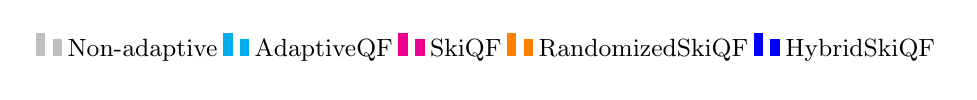
\begin{tikzpicture}
\begin{axis}[hide axis,xmin=0,xmax=1,ymin=0,ymax=1,
scale only axis,width=1cm,height=0.4cm,
legend columns=5,legend cell align=left,
legend style={draw=none,font=\small,at={(0.5,0.5)},anchor=center}]
\addlegendimage{ybar legend,/tikz/ybar,skiqfNonAdaptiveBar}
\addlegendentry{Non-adaptive}
\addlegendimage{ybar legend,/tikz/ybar,skiqfAdaptiveBar}
\addlegendentry{AdaptiveQF}
\addlegendimage{ybar legend,/tikz/ybar,skiqfSkiBar}
\addlegendentry{SkiQF}
\addlegendimage{ybar legend,/tikz/ybar,skiqfRandomizedBar}
\addlegendentry{RandomizedSkiQF}
\addlegendimage{ybar legend,/tikz/ybar,skiqfHybridBar}
\addlegendentry{HybridSkiQF}
\end{axis}\end{tikzpicture}
\par\medskip
\begingroup
\pgfmathsetlengthmacro{\skiqfpanelwidth}{(\linewidth-1.6cm-1.3cm)/2}
\begin{tikzpicture}\begin{groupplot}[skiqf axis,
group style={group size=2 by 1,horizontal sep=1.3cm,vertical sep=1.5cm},
scale only axis,width=\skiqfpanelwidth,height=3cm,scaled y ticks=true]
\nextgroupplot[title={Overall throughput},
ylabel={Throughput\\(MOps/sec)},
ymin=0,
ybar=0,bar width=5pt,enlarge x limits=false,
xmin=-0.5,xmax=0.5,
xtick={0},
xticklabels={Immediate feedback},
x tick label style={rotate=45,anchor=east,font=\scriptsize}]
\addplot[skiqfNonAdaptiveBar,mark size=1.8pt,mark repeat=1] coordinates {(0,0.158388)};
\addplot[skiqfAdaptiveBar,mark size=1.8pt,mark repeat=1] coordinates {(0,1.191532)};
\addplot[skiqfSkiBar,mark size=1.8pt,mark repeat=1] coordinates {(0,0.856136)};
\addplot[skiqfRandomizedBar,mark size=1.8pt,mark repeat=1] coordinates {(0,0.938719)};
\addplot[skiqfHybridBar,mark size=1.8pt,mark repeat=1] coordinates {(0,0.390469)};
\nextgroupplot[title={Overall FPR},
ylabel={False positive rate},
ymin=0,
ybar=0,bar width=5pt,enlarge x limits=false,
xmin=-0.5,xmax=0.5,
xtick={0},
xticklabels={Immediate feedback},
x tick label style={rotate=45,anchor=east,font=\scriptsize}]
\addplot[skiqfNonAdaptiveBar,mark size=1.8pt,mark repeat=1] coordinates {(0,0.0533292)};
\addplot[skiqfAdaptiveBar,mark size=1.8pt,mark repeat=1] coordinates {(0,0.0034942)};
\addplot[skiqfSkiBar,mark size=1.8pt,mark repeat=1] coordinates {(0,0.006850966667)};
\addplot[skiqfRandomizedBar,mark size=1.8pt,mark repeat=1] coordinates {(0,0.005744433333)};
\addplot[skiqfHybridBar,mark size=1.8pt,mark repeat=1] coordinates {(0,0.0200778)};
\end{groupplot}\end{tikzpicture}\endgroup\end{center}

\begin{center}\small Final cumulative measurements. Throughput: higher is better; FPR: lower is better.\end{center}
\subsection*{Large results}
All ten cases completed. Each measurement is from one run.\par
distributions/uniform: singleton keys 100.00\%, singleton operations 100.00\%; initial-FP singleton keys 100.00\%; randomized/deterministic throughput 0.781.\par
distributions/normal: singleton keys 4.42\%, singleton operations 0.88\%; initial-FP singleton keys 4.52\%; randomized/deterministic throughput 1.108.\par
distributions/lognormal: singleton keys 32.64\%, singleton operations 9.42\%; initial-FP singleton keys 32.59\%; randomized/deterministic throughput 1.044.\par
distributions/zipf: singleton keys 71.09\%, singleton operations 13.32\%; initial-FP singleton keys 71.24\%; randomized/deterministic throughput 0.932.\par
singleton-mixture/f-000: singleton keys 0.00\%, singleton operations 0.00\%; initial-FP singleton keys 0.00\%; randomized/deterministic throughput 1.100.\par
singleton-mixture/f-025: singleton keys 25.00\%, singleton operations 14.29\%; initial-FP singleton keys 25.03\%; randomized/deterministic throughput 1.052.\par
singleton-mixture/f-050: singleton keys 50.00\%, singleton operations 33.33\%; initial-FP singleton keys 50.11\%; randomized/deterministic throughput 1.008.\par
singleton-mixture/f-075: singleton keys 75.00\%, singleton operations 60.00\%; initial-FP singleton keys 75.05\%; randomized/deterministic throughput 0.895.\par
singleton-mixture/f-100: singleton keys 100.00\%, singleton operations 100.00\%; initial-FP singleton keys 100.00\%; randomized/deterministic throughput 0.745.\par
\clearpage
\section{Singleton mixtures}
The horizontal axis is the fraction of distinct keys appearing once; all other keys appear twice.
\begin{center}
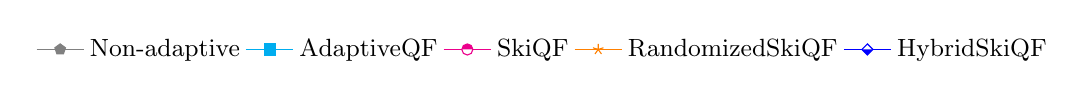
\begin{tikzpicture}
\begin{axis}[hide axis,xmin=0,xmax=1,ymin=0,ymax=1,
scale only axis,width=1cm,height=0.4cm,
legend columns=5,legend cell align=left,
legend style={draw=none,font=\small,at={(0.5,0.5)},anchor=center}]
\addlegendimage{skiqfNonAdaptive}
\addlegendentry{Non-adaptive}
\addlegendimage{skiqfAdaptive}
\addlegendentry{AdaptiveQF}
\addlegendimage{skiqfSki}
\addlegendentry{SkiQF}
\addlegendimage{skiqfRandomized}
\addlegendentry{RandomizedSkiQF}
\addlegendimage{skiqfHybrid}
\addlegendentry{HybridSkiQF}
\end{axis}\end{tikzpicture}
\par\medskip
\begingroup
\pgfmathsetlengthmacro{\skiqfpanelwidth}{(\linewidth-1.6cm-1.3cm)/2}
\begin{tikzpicture}\begin{groupplot}[skiqf axis,
group style={group size=2 by 2,horizontal sep=1.3cm,vertical sep=1.5cm},
scale only axis,width=\skiqfpanelwidth,height=3cm,scaled y ticks=true]
\nextgroupplot[title={Throughput (MOps/s)},
ylabel={Throughput (MOps/s)},
ymin=0,
xlabel={Singleton fraction}]
\addplot[skiqfNonAdaptive,mark size=1.8pt,mark repeat=1] coordinates {(0,1.799041) (0.25,1.805794) (0.5,1.798787) (0.75,1.819765) (1,1.799054)};
\addplot[skiqfAdaptive,mark size=1.8pt,mark repeat=1] coordinates {(0,1.752622) (0.25,1.561684) (0.5,1.246321) (0.75,1.162634) (1,0.921182)};
\addplot[skiqfSki,mark size=1.8pt,mark repeat=1] coordinates {(0,1.247593) (0.25,1.304077) (0.5,1.370921) (0.75,1.53509) (1,1.841932)};
\addplot[skiqfRandomized,mark size=1.8pt,mark repeat=1] coordinates {(0,1.37192) (0.25,1.372456) (0.5,1.381746) (0.75,1.3745) (1,1.37307)};
\addplot[skiqfHybrid,mark size=1.8pt,mark repeat=1] coordinates {(0,1.748928) (0.25,1.556124) (0.5,1.293267) (0.75,1.151042) (1,1.801418)};
\nextgroupplot[title={Observed FPR},
ylabel={Observed FPR},
ymin=0,
xlabel={Singleton fraction}]
\addplot[skiqfNonAdaptive,mark size=1.8pt,mark repeat=1] coordinates {(0,0.0035162) (0.25,0.00351152) (0.5,0.0035091) (0.75,0.00350904) (1,0.00350736)};
\addplot[skiqfAdaptive,mark size=1.8pt,mark repeat=1] coordinates {(0,0.00175965) (0.25,0.00200773) (0.5,0.00234079) (0.75,0.00280619) (1,0.00350195)};
\addplot[skiqfSki,mark size=1.8pt,mark repeat=1] coordinates {(0,0.00351356) (0.25,0.003509) (0.5,0.00350676) (0.75,0.00350735) (1,0.00350736)};
\addplot[skiqfRandomized,mark size=1.8pt,mark repeat=1] coordinates {(0,0.00293425) (0.25,0.00301226) (0.5,0.00312073) (0.75,0.00327295) (1,0.00350555)};
\addplot[skiqfHybrid,mark size=1.8pt,mark repeat=1] coordinates {(0,0.00179477) (0.25,0.00203806) (0.5,0.00236472) (0.75,0.00282008) (1,0.00350736)};
\nextgroupplot[title={Adaptations},
ylabel={Adaptations},
ymin=0,
xlabel={Singleton fraction}]
\addplot[skiqfNonAdaptive,mark size=1.8pt,mark repeat=1] coordinates {(0,0) (0.25,0) (0.5,0) (0.75,0) (1,0)};
\addplot[skiqfAdaptive,mark size=1.8pt,mark repeat=1] coordinates {(0,175965) (0.25,200773) (0.5,234079) (0.75,280619) (1,350195)};
\addplot[skiqfSki,mark size=1.8pt,mark repeat=1] coordinates {(0,175678) (0.25,150376) (0.5,116805) (0.75,70241) (1,542)};
\addplot[skiqfRandomized,mark size=1.8pt,mark repeat=1] coordinates {(0,175706) (0.25,167145) (0.5,155752) (0.75,139990) (1,116736)};
\addplot[skiqfHybrid,mark size=1.8pt,mark repeat=1] coordinates {(0,175938) (0.25,200245) (0.5,232881) (0.75,278455) (1,0)};
\nextgroupplot[title={Physical reads (MiB)},
ylabel={Physical reads (MiB)},
ymin=0,
xlabel={Singleton fraction}]
\addplot[skiqfNonAdaptive,mark size=1.8pt,mark repeat=1] coordinates {(0,9455.78125) (0.25,9445.410156) (0.5,9445.027344) (0.75,9453.742188) (1,9462.097656)};
\addplot[skiqfAdaptive,mark size=1.8pt,mark repeat=1] coordinates {(0,7904.886719) (0.25,9019.488281) (0.5,10530.34766) (0.75,12599.77734) (1,15728.29297)};
\addplot[skiqfSki,mark size=1.8pt,mark repeat=1] coordinates {(0,12441.38672) (0.25,11967.61719) (0.5,11330.375) (0.75,10460.0625) (1,9158.171875)};
\addplot[skiqfRandomized,mark size=1.8pt,mark repeat=1] coordinates {(0,10938.69922) (0.25,10983.79688) (0.5,11078.67578) (0.75,11170.26953) (1,11347.90234)};
\addplot[skiqfHybrid,mark size=1.8pt,mark repeat=1] coordinates {(0,8035.351562) (0.25,9110.859375) (0.5,10575.67188) (0.75,12592.08203) (1,9151.691406)};
\end{groupplot}\end{tikzpicture}\endgroup\end{center}

\begin{center}\small Single-run results; no error bars.\end{center}
\clearpage
\section{Robustness across workload distributions}
Distribution panels and aggregate comparisons follow the paper's robustness study.
\begin{center}
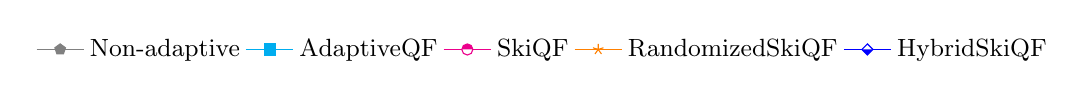
\begin{tikzpicture}
\begin{axis}[hide axis,xmin=0,xmax=1,ymin=0,ymax=1,
scale only axis,width=1cm,height=0.4cm,
legend columns=5,legend cell align=left,
legend style={draw=none,font=\small,at={(0.5,0.5)},anchor=center}]
\addlegendimage{skiqfNonAdaptive}
\addlegendentry{Non-adaptive}
\addlegendimage{skiqfAdaptive}
\addlegendentry{AdaptiveQF}
\addlegendimage{skiqfSki}
\addlegendentry{SkiQF}
\addlegendimage{skiqfRandomized}
\addlegendentry{RandomizedSkiQF}
\addlegendimage{skiqfHybrid}
\addlegendentry{HybridSkiQF}
\end{axis}\end{tikzpicture}
\par\medskip
\begingroup
\pgfmathsetlengthmacro{\skiqfpanelwidth}{(\linewidth-1.6cm-2.0999999999999996cm)/4}
\begin{tikzpicture}\begin{groupplot}[skiqf axis,
group style={group size=4 by 1,horizontal sep=0.7cm,vertical sep=1.5cm},
scale only axis,width=\skiqfpanelwidth,height=3cm,scaled y ticks=true]
\nextgroupplot[title={Uniform},
ylabel={Throughput\\(MOps/sec)},
ymin=0,
xlabel={Queries (millions)},
xmin=0,xmax=100,enlarge x limits=false]
\addplot[skiqfNonAdaptive,mark size=1.8pt,mark repeat=11] coordinates {(1,1.629355) (2,1.85226) (3,1.834647) (4,1.815585) (5,1.839038) (6,1.817807) (7,1.853765) (8,1.808456) (9,1.816661) (10,1.775378) (11,1.861421) (12,1.784706) (13,1.808676) (14,1.858467) (15,1.82339) (16,1.812272) (17,1.778771) (18,1.835988) (19,1.779997) (20,1.86992) (21,1.82897) (22,1.794898) (23,1.827142) (24,1.850259) (25,1.719517) (26,1.823304) (27,1.794445) (28,1.841531) (29,1.900757) (30,1.814815) (31,1.879603) (32,1.836408) (33,1.842799) (34,1.771971) (35,1.831945) (36,1.786269) (37,1.84582) (38,1.827041) (39,1.813704) (40,1.835112) (41,1.835735) (42,1.79426) (43,1.789181) (44,1.870386) (45,1.803768) (46,1.803564) (47,1.845454) (48,1.834666) (49,1.872443) (50,1.831315) (51,1.82595) (52,1.838632) (53,1.772232) (54,1.860593) (55,1.886742) (56,1.794293) (57,1.717498) (58,1.879367) (59,1.791929) (60,1.864039) (61,1.821502) (62,1.82731) (63,1.827278) (64,1.801283) (65,1.822563) (66,1.734471) (67,1.68884) (68,1.794003) (69,1.751071) (70,1.872244) (71,1.839884) (72,1.82728) (73,1.719083) (74,1.835494) (75,1.779342) (76,1.779117) (77,1.9187) (78,1.835997) (79,1.814625) (80,1.802543) (81,1.809851) (82,1.78679) (83,1.722471) (84,1.880128) (85,1.854827) (86,1.769344) (87,1.822301) (88,1.876093) (89,1.878332) (90,1.880068) (91,1.829496) (92,1.812168) (93,1.789805) (94,1.768111) (95,1.897753) (96,1.802099) (97,1.842008) (98,1.851703) (99,1.857136) (100,1.771598)};
\addplot[skiqfAdaptive,mark size=1.8pt,mark repeat=11] coordinates {(1,0.963911) (2,0.949914) (3,0.94423) (4,0.958671) (5,0.903749) (6,0.957591) (7,0.925558) (8,0.969393) (9,0.965676) (10,0.941876) (11,0.951415) (12,0.942364) (13,0.934455) (14,0.980873) (15,0.959982) (16,0.965366) (17,0.93682) (18,0.949521) (19,0.954803) (20,0.960814) (21,0.970659) (22,0.956272) (23,0.948031) (24,0.935101) (25,0.927428) (26,0.940059) (27,0.941019) (28,0.924455) (29,0.979006) (30,0.948296) (31,0.947338) (32,0.941697) (33,0.944626) (34,0.938064) (35,0.930921) (36,0.936687) (37,0.933796) (38,0.925934) (39,0.949076) (40,0.956957) (41,0.969639) (42,0.954223) (43,0.968838) (44,0.98709) (45,0.948813) (46,0.921568) (47,0.954632) (48,0.936693) (49,0.965966) (50,0.86793) (51,0.777143) (52,0.753251) (53,0.738853) (54,0.84387) (55,0.811979) (56,0.781165) (57,0.771985) (58,0.74524) (59,0.713354) (60,0.755532) (61,0.737048) (62,0.783704) (63,0.749823) (64,0.809941) (65,0.678053) (66,0.782901) (67,0.800125) (68,0.685453) (69,0.727803) (70,0.746462) (71,0.703295) (72,0.708757) (73,0.781566) (74,0.737689) (75,0.872745) (76,0.758777) (77,0.850079) (78,0.784266) (79,0.739418) (80,0.821921) (81,0.86796) (82,0.797676) (83,0.692286) (84,0.77826) (85,0.775806) (86,0.712586) (87,0.809843) (88,0.789998) (89,0.796307) (90,0.712334) (91,0.763992) (92,0.738462) (93,0.752451) (94,0.702716) (95,0.713822) (96,0.77411) (97,0.70533) (98,0.766946) (99,0.758801) (100,0.732327)};
\addplot[skiqfSki,mark size=1.8pt,mark repeat=11] coordinates {(1,2.118824) (2,1.763632) (3,1.815985) (4,1.818007) (5,1.747799) (6,1.79489) (7,1.689226) (8,1.781894) (9,1.768293) (10,1.784762) (11,1.818607) (12,1.786268) (13,1.831794) (14,1.842308) (15,1.81095) (16,1.779007) (17,1.758032) (18,1.688573) (19,1.812747) (20,1.814686) (21,1.753998) (22,1.64313) (23,1.715155) (24,1.708552) (25,1.6732) (26,1.533418) (27,1.64374) (28,1.722124) (29,1.708728) (30,1.753955) (31,1.825199) (32,1.683365) (33,1.662314) (34,1.504492) (35,1.650364) (36,1.711541) (37,1.643656) (38,1.667627) (39,1.663272) (40,1.689904) (41,1.734591) (42,1.60229) (43,1.695766) (44,1.793788) (45,1.67854) (46,1.643558) (47,1.673302) (48,1.83327) (49,1.851797) (50,1.805824) (51,1.830241) (52,1.864201) (53,1.787319) (54,1.829569) (55,1.859205) (56,1.704482) (57,1.729179) (58,1.80602) (59,1.800872) (60,1.864074) (61,1.799447) (62,1.823996) (63,1.835385) (64,1.856862) (65,1.795244) (66,1.681192) (67,1.79994) (68,1.76003) (69,1.805093) (70,1.83034) (71,1.811156) (72,1.799592) (73,1.794741) (74,1.801166) (75,1.807133) (76,1.787552) (77,1.85647) (78,1.782891) (79,1.774044) (80,1.786085) (81,1.806835) (82,1.812) (83,1.756421) (84,1.817451) (85,1.818512) (86,1.800495) (87,1.81183) (88,1.833347) (89,1.847457) (90,1.794459) (91,1.715043) (92,1.76318) (93,1.831867) (94,1.772393) (95,1.799145) (96,1.796271) (97,1.680947) (98,1.666824) (99,1.777036) (100,1.58826)};
\addplot[skiqfRandomized,mark size=1.8pt,mark repeat=11] coordinates {(1,1.415376) (2,1.394368) (3,1.432744) (4,1.430995) (5,1.440412) (6,1.409375) (7,1.411467) (8,1.438234) (9,1.430955) (10,1.390931) (11,1.438852) (12,1.382742) (13,1.406658) (14,1.453231) (15,1.41141) (16,1.419732) (17,1.356955) (18,1.262152) (19,1.283568) (20,1.423135) (21,1.383751) (22,1.401935) (23,1.443143) (24,1.42268) (25,1.401154) (26,1.405826) (27,1.393349) (28,1.409367) (29,1.422431) (30,1.367159) (31,1.414451) (32,1.412409) (33,1.417124) (34,1.32655) (35,1.357189) (36,1.365935) (37,1.399583) (38,1.3942) (39,1.379312) (40,1.386784) (41,1.414781) (42,1.376083) (43,1.409885) (44,1.456765) (45,1.382889) (46,1.341326) (47,1.355224) (48,1.369538) (49,1.441065) (50,1.383395) (51,1.406696) (52,1.412027) (53,1.292367) (54,1.417721) (55,1.445165) (56,1.360372) (57,1.345836) (58,1.397747) (59,1.369623) (60,1.45539) (61,1.392904) (62,1.402825) (63,1.415679) (64,1.438144) (65,1.398682) (66,1.405649) (67,1.387449) (68,1.372184) (69,1.398413) (70,1.428841) (71,1.404893) (72,1.406168) (73,1.387383) (74,1.350167) (75,1.329186) (76,1.343088) (77,1.386146) (78,1.323382) (79,1.3467) (80,1.38205) (81,1.324336) (82,1.325231) (83,1.289199) (84,1.285856) (85,1.316158) (86,1.361938) (87,1.299356) (88,1.250252) (89,1.3943) (90,1.377474) (91,1.31027) (92,1.284401) (93,1.368772) (94,1.331617) (95,1.255497) (96,1.342174) (97,1.347972) (98,1.350259) (99,1.321456) (100,1.157067)};
\addplot[skiqfHybrid,mark size=1.8pt,mark repeat=11] coordinates {(1,1.661537) (2,1.82073) (3,1.844382) (4,1.802457) (5,1.823417) (6,1.853566) (7,1.863688) (8,1.818452) (9,1.878982) (10,1.820532) (11,1.854292) (12,1.800625) (13,1.839558) (14,1.911561) (15,1.872483) (16,1.856812) (17,1.834932) (18,1.845555) (19,1.855154) (20,1.889889) (21,1.869246) (22,1.854587) (23,1.842559) (24,1.829894) (25,1.730263) (26,1.758773) (27,1.788734) (28,1.822568) (29,1.859048) (30,1.833061) (31,1.840365) (32,1.798594) (33,1.803752) (34,1.838192) (35,1.773957) (36,1.796023) (37,1.787929) (38,1.855114) (39,1.829859) (40,1.824076) (41,1.848719) (42,1.848943) (43,1.825456) (44,1.748599) (45,1.723033) (46,1.756264) (47,1.807101) (48,1.83254) (49,1.830692) (50,1.807194) (51,1.838131) (52,1.828153) (53,1.686664) (54,1.781447) (55,1.819385) (56,1.727223) (57,1.732502) (58,1.785793) (59,1.792683) (60,1.910023) (61,1.808924) (62,1.804022) (63,1.841844) (64,1.897891) (65,1.778796) (66,1.802098) (67,1.802532) (68,1.768591) (69,1.828474) (70,1.81559) (71,1.815474) (72,1.830871) (73,1.77229) (74,1.806677) (75,1.851071) (76,1.831041) (77,1.910576) (78,1.865238) (79,1.827418) (80,1.769519) (81,1.841467) (82,1.825525) (83,1.768414) (84,1.852497) (85,1.821963) (86,1.826129) (87,1.821093) (88,1.877713) (89,1.826858) (90,1.79652) (91,1.837163) (92,1.753316) (93,1.766527) (94,1.833344) (95,1.88999) (96,1.737419) (97,1.799027) (98,1.81955) (99,1.843306) (100,1.697381)};
\nextgroupplot[title={Normal},
ymin=0,
xlabel={Queries (millions)},
xmin=0,xmax=100,enlarge x limits=false]
\addplot[skiqfNonAdaptive,mark size=1.8pt,mark repeat=11] coordinates {(1,1.658015) (2,1.862665) (3,1.829464) (4,1.854519) (5,1.919791) (6,1.890354) (7,1.880456) (8,1.825288) (9,1.895352) (10,1.787252) (11,1.799905) (12,1.88083) (13,1.861274) (14,1.976767) (15,2.542879) (16,1.971938) (17,1.870721) (18,1.861106) (19,1.81605) (20,1.871451) (21,1.845418) (22,1.812535) (23,1.917039) (24,1.872834) (25,1.838628) (26,1.85454) (27,1.810027) (28,1.940495) (29,1.828767) (30,1.843302) (31,1.82765) (32,1.780644) (33,1.864947) (34,1.790663) (35,1.898648) (36,1.841004) (37,1.877231) (38,1.816066) (39,1.849817) (40,1.881107) (41,1.886309) (42,1.90126) (43,1.803568) (44,1.814269) (45,1.856866) (46,1.839611) (47,1.829066) (48,1.812049) (49,1.830598) (50,1.891394) (51,1.883682) (52,1.888959) (53,1.832791) (54,1.938129) (55,1.896283) (56,1.908525) (57,1.843976) (58,1.869114) (59,1.89998) (60,1.876492) (61,1.860572) (62,1.895635) (63,1.893241) (64,1.919773) (65,1.746342) (66,1.836004) (67,1.816927) (68,1.90197) (69,1.904824) (70,1.846737) (71,1.854646) (72,1.871478) (73,1.909523) (74,1.819106) (75,1.784591) (76,1.823484) (77,1.83099) (78,1.87758) (79,1.791427) (80,1.84858) (81,1.877399) (82,1.823986) (83,1.814277) (84,1.873614) (85,1.811289) (86,1.881631) (87,1.882672) (88,1.690971) (89,1.895074) (90,1.894869) (91,1.869323) (92,1.810956) (93,1.810576) (94,1.865252) (95,1.844413) (96,1.89924) (97,1.844943) (98,1.849176) (99,1.804043) (100,1.902412)};
\addplot[skiqfAdaptive,mark size=1.8pt,mark repeat=11] coordinates {(1,0.91526) (2,1.019628) (3,1.070849) (4,1.156172) (5,1.213286) (6,1.263382) (7,1.279701) (8,1.342741) (9,1.371246) (10,1.4151) (11,1.473031) (12,1.637585) (13,1.7149) (14,1.812982) (15,1.839425) (16,1.912254) (17,1.989959) (18,2.092574) (19,2.158224) (20,2.270204) (21,2.314702) (22,2.483253) (23,2.588453) (24,2.56781) (25,2.70726) (26,2.907754) (27,2.98732) (28,3.161997) (29,3.159087) (30,3.142167) (31,3.830917) (32,3.479257) (33,3.601596) (34,3.835576) (35,3.912169) (36,4.080887) (37,4.242399) (38,4.276002) (39,4.335885) (40,4.396387) (41,4.691365) (42,4.83378) (43,5.067998) (44,4.866758) (45,5.053729) (46,5.748313) (47,5.345778) (48,5.936336) (49,5.844186) (50,6.310562) (51,6.255717) (52,6.524436) (53,6.31602) (54,6.101218) (55,7.090778) (56,7.349144) (57,6.896534) (58,7.388743) (59,7.269977) (60,7.685796) (61,7.496934) (62,7.248455) (63,7.671964) (64,8.275852) (65,8.391998) (66,7.862324) (67,8.728016) (68,8.201847) (69,8.993333) (70,7.817454) (71,8.380507) (72,9.537637) (73,7.674582) (74,9.018338) (75,9.484612) (76,8.570387) (77,8.422546) (78,7.789516) (79,9.721494) (80,9.333395) (81,8.426647) (82,10.112325) (83,7.637295) (84,10.089564) (85,10.363193) (86,10.847452) (87,10.105787) (88,10.621305) (89,10.260157) (90,10.878591) (91,10.202482) (92,10.893976) (93,10.341408) (94,11.011407) (95,11.083129) (96,9.379468) (97,9.880416) (98,11.177968) (99,11.224049) (100,11.260033)};
\addplot[skiqfSki,mark size=1.8pt,mark repeat=11] coordinates {(1,2.092808) (2,1.741093) (3,1.698196) (4,1.685203) (5,1.667868) (6,1.549731) (7,1.518222) (8,1.544966) (9,1.562643) (10,1.456977) (11,1.496272) (12,1.561778) (13,1.489073) (14,1.571931) (15,1.504353) (16,1.476141) (17,1.587429) (18,1.588043) (19,1.546108) (20,1.640861) (21,1.707006) (22,1.684225) (23,1.790604) (24,1.645847) (25,1.77375) (26,1.852262) (27,1.68855) (28,1.980292) (29,2.005944) (30,1.724995) (31,1.847811) (32,1.725912) (33,2.113036) (34,1.765463) (35,2.027192) (36,1.970683) (37,2.255921) (38,2.184626) (39,2.284679) (40,2.474235) (41,2.518163) (42,2.345044) (43,2.565509) (44,2.73828) (45,2.591367) (46,2.438437) (47,2.815121) (48,2.738038) (49,3.009721) (50,3.08957) (51,2.846304) (52,3.459381) (53,3.377389) (54,2.935598) (55,3.726246) (56,3.691396) (57,3.619399) (58,3.449147) (59,3.559854) (60,3.638667) (61,4.034604) (62,4.287391) (63,4.322799) (64,3.885247) (65,3.926427) (66,4.523451) (67,4.337305) (68,4.701404) (69,4.917391) (70,4.156399) (71,5.142178) (72,5.341832) (73,5.197021) (74,5.238561) (75,4.883808) (76,5.526514) (77,5.461109) (78,6.064229) (79,5.876203) (80,5.340075) (81,6.37256) (82,5.991447) (83,5.66716) (84,6.437617) (85,6.567272) (86,6.94346) (87,7.117696) (88,6.752047) (89,7.295082) (90,5.549325) (91,6.702492) (92,7.081153) (93,7.031778) (94,7.884267) (95,7.649027) (96,6.449736) (97,7.206919) (98,7.868141) (99,7.635499) (100,6.666111)};
\addplot[skiqfRandomized,mark size=1.8pt,mark repeat=11] coordinates {(1,1.268862) (2,1.393737) (3,1.449132) (4,1.463235) (5,1.48132) (6,1.457335) (7,1.480424) (8,1.477558) (9,1.531127) (10,1.413584) (11,1.492414) (12,1.585954) (13,1.647715) (14,1.64887) (15,1.618334) (16,1.668991) (17,1.751481) (18,1.78841) (19,1.79231) (20,1.873989) (21,1.89808) (22,1.888519) (23,1.96689) (24,1.930741) (25,2.140272) (26,2.174394) (27,2.119792) (28,2.275305) (29,2.198826) (30,2.221265) (31,2.4575) (32,2.476446) (33,2.462988) (34,2.511996) (35,2.432614) (36,2.556282) (37,2.727747) (38,2.593444) (39,2.93048) (40,2.965853) (41,2.921092) (42,2.936249) (43,3.015829) (44,2.982725) (45,3.239802) (46,3.38982) (47,3.421847) (48,3.631622) (49,3.304378) (50,3.732823) (51,3.594214) (52,3.996343) (53,4.03884) (54,4.161035) (55,4.09212) (56,4.243306) (57,4.10422) (58,4.65346) (59,4.271273) (60,4.753277) (61,4.79769) (62,4.534859) (63,5.09389) (64,5.464357) (65,5.489945) (66,5.601661) (67,5.199277) (68,4.571484) (69,5.18038) (70,5.196394) (71,5.74716) (72,5.609118) (73,6.344802) (74,6.23333) (75,6.053155) (76,6.596084) (77,6.432569) (78,6.865762) (79,6.802765) (80,6.936) (81,6.868034) (82,7.106172) (83,6.979828) (84,6.822216) (85,7.300352) (86,7.296704) (87,5.633784) (88,6.093125) (89,6.88813) (90,7.074615) (91,8.040881) (92,6.278771) (93,7.534246) (94,8.844332) (95,8.853338) (96,7.736346) (97,8.527193) (98,8.246951) (99,8.426063) (100,9.246419)};
\addplot[skiqfHybrid,mark size=1.8pt,mark repeat=11] coordinates {(1,1.568122) (2,0.938142) (3,0.913356) (4,0.994086) (5,1.09449) (6,1.145258) (7,1.165213) (8,1.230942) (9,1.323282) (10,1.365586) (11,1.395606) (12,1.506639) (13,1.457398) (14,1.518289) (15,1.645356) (16,1.669296) (17,1.996502) (18,1.749514) (19,2.023429) (20,1.923965) (21,2.229153) (22,2.354942) (23,2.224848) (24,2.532609) (25,2.531413) (26,2.72235) (27,2.848009) (28,2.520159) (29,3.03335) (30,2.621968) (31,3.450995) (32,3.363389) (33,3.572798) (34,3.649759) (35,3.508526) (36,3.894287) (37,4.089979) (38,4.032979) (39,4.173176) (40,4.420641) (41,4.405162) (42,4.520746) (43,4.896974) (44,4.618253) (45,4.392663) (46,5.460754) (47,4.543778) (48,5.667939) (49,5.646094) (50,5.644098) (51,4.985204) (52,6.332892) (53,5.436186) (54,6.810713) (55,6.821065) (56,6.738569) (57,6.700199) (58,7.297433) (59,7.193037) (60,5.661852) (61,5.690948) (62,7.375052) (63,6.74415) (64,6.689659) (65,8.126694) (66,8.348915) (67,8.304562) (68,8.224121) (69,7.416516) (70,6.602739) (71,8.407544) (72,9.29225) (73,8.901927) (74,9.298355) (75,9.209181) (76,9.512988) (77,8.396856) (78,9.420899) (79,7.809088) (80,8.973312) (81,10.022222) (82,9.966138) (83,9.901915) (84,9.921946) (85,10.144327) (86,10.350687) (87,9.873359) (88,8.835101) (89,9.19035) (90,10.200351) (91,10.753241) (92,10.711099) (93,10.818193) (94,11.151271) (95,10.898252) (96,9.466482) (97,8.83092) (98,10.284216) (99,11.231367) (100,9.429759)};
\nextgroupplot[title={Lognormal},
ymin=0,
xlabel={Queries (millions)},
xmin=0,xmax=100,enlarge x limits=false]
\addplot[skiqfNonAdaptive,mark size=1.8pt,mark repeat=11] coordinates {(1,1.679797) (2,1.855175) (3,1.856418) (4,1.880584) (5,1.865219) (6,1.883833) (7,1.845166) (8,1.932703) (9,1.897383) (10,1.859827) (11,1.904742) (12,1.90641) (13,1.894093) (14,1.851988) (15,1.867248) (16,1.832032) (17,1.791629) (18,1.874022) (19,1.837104) (20,1.765887) (21,1.786519) (22,1.642715) (23,1.859408) (24,1.888201) (25,1.751034) (26,1.856253) (27,1.894599) (28,1.662159) (29,1.811101) (30,1.82847) (31,1.813476) (32,1.918608) (33,1.831794) (34,1.902784) (35,1.918495) (36,1.877466) (37,1.836098) (38,1.886438) (39,1.817896) (40,1.865534) (41,1.818375) (42,1.840892) (43,1.842563) (44,1.856448) (45,1.85839) (46,1.866068) (47,1.8912) (48,1.830969) (49,1.598341) (50,1.906592) (51,1.783393) (52,1.735028) (53,1.859975) (54,1.833294) (55,1.817206) (56,1.869356) (57,1.899404) (58,1.845118) (59,1.800119) (60,1.876088) (61,1.840147) (62,1.824805) (63,1.840608) (64,1.801951) (65,1.876979) (66,1.888866) (67,1.824359) (68,1.849594) (69,1.917186) (70,1.855239) (71,1.905271) (72,1.85903) (73,1.881447) (74,1.810794) (75,1.805779) (76,1.885447) (77,1.880039) (78,1.866264) (79,1.79043) (80,1.864867) (81,1.80017) (82,1.757142) (83,1.816023) (84,1.833403) (85,1.859894) (86,1.855009) (87,1.903305) (88,1.841564) (89,1.894411) (90,1.855831) (91,1.874893) (92,1.898757) (93,1.851806) (94,1.834342) (95,1.898038) (96,1.844512) (97,1.839048) (98,1.844101) (99,1.892798) (100,1.88346)};
\addplot[skiqfAdaptive,mark size=1.8pt,mark repeat=11] coordinates {(1,0.890197) (2,1.026299) (3,1.116881) (4,1.149834) (5,1.203903) (6,1.257617) (7,1.194386) (8,1.396057) (9,1.448279) (10,1.462235) (11,1.542481) (12,1.588171) (13,1.650454) (14,1.656942) (15,1.756255) (16,1.78562) (17,1.850966) (18,1.817661) (19,1.869266) (20,1.875121) (21,1.950789) (22,1.992726) (23,2.105645) (24,2.140228) (25,2.183562) (26,2.218181) (27,2.395687) (28,2.341091) (29,2.460218) (30,2.427121) (31,2.49345) (32,2.66977) (33,2.574632) (34,2.797812) (35,2.882599) (36,2.763313) (37,2.764814) (38,2.951947) (39,2.700567) (40,2.949135) (41,2.916369) (42,3.067158) (43,3.156737) (44,3.226598) (45,3.349803) (46,3.384827) (47,3.418341) (48,2.636652) (49,3.390533) (50,3.507022) (51,3.612868) (52,3.604314) (53,3.743887) (54,3.018752) (55,3.599041) (56,3.779608) (57,3.858398) (58,3.969296) (59,3.635033) (60,3.934821) (61,3.850394) (62,3.822636) (63,3.870894) (64,4.077139) (65,4.046013) (66,4.36741) (67,4.131979) (68,3.900369) (69,3.952457) (70,4.392048) (71,4.276438) (72,4.375908) (73,4.338282) (74,4.049751) (75,4.23719) (76,4.710755) (77,4.625153) (78,4.579211) (79,4.335463) (80,5.131155) (81,4.816948) (82,4.808438) (83,5.067616) (84,4.969146) (85,4.942658) (86,4.767292) (87,5.1904) (88,5.507187) (89,4.909924) (90,5.557663) (91,5.240577) (92,5.507062) (93,5.550626) (94,5.240803) (95,5.495111) (96,5.600442) (97,4.650264) (98,5.605443) (99,4.854067) (100,6.035736)};
\addplot[skiqfSki,mark size=1.8pt,mark repeat=11] coordinates {(1,1.60896) (2,1.69579) (3,1.758919) (4,1.666723) (5,1.644322) (6,1.598631) (7,1.661984) (8,1.738758) (9,1.694786) (10,1.720103) (11,1.715273) (12,1.694946) (13,1.719207) (14,1.734756) (15,1.680333) (16,1.785096) (17,1.819802) (18,1.834108) (19,1.826359) (20,1.832651) (21,1.864257) (22,1.841142) (23,1.880839) (24,1.929295) (25,1.809943) (26,1.998087) (27,2.062384) (28,1.962098) (29,2.077187) (30,2.068873) (31,2.161039) (32,2.2376) (33,2.190619) (34,2.142899) (35,2.321375) (36,2.289438) (37,2.231844) (38,2.431126) (39,2.16844) (40,2.31336) (41,2.220504) (42,2.365122) (43,2.524323) (44,2.431238) (45,2.442301) (46,2.658353) (47,2.558973) (48,2.396177) (49,2.568414) (50,2.706531) (51,2.672338) (52,2.63987) (53,2.695155) (54,2.755105) (55,2.850095) (56,2.822156) (57,2.644179) (58,2.887016) (59,2.650565) (60,2.885477) (61,3.076167) (62,2.839144) (63,2.898978) (64,2.963037) (65,3.037127) (66,3.12111) (67,2.899346) (68,3.132228) (69,3.190096) (70,3.041804) (71,3.030142) (72,3.216345) (73,3.297409) (74,3.292064) (75,3.419474) (76,3.270619) (77,3.288474) (78,3.541031) (79,3.362539) (80,3.511488) (81,3.383674) (82,3.41905) (83,3.582951) (84,3.650212) (85,3.499634) (86,3.578813) (87,3.819745) (88,3.680514) (89,3.820627) (90,3.686038) (91,3.586211) (92,3.747259) (93,3.882865) (94,3.648362) (95,3.833688) (96,4.003125) (97,4.022407) (98,3.971258) (99,3.724731) (100,3.946654)};
\addplot[skiqfRandomized,mark size=1.8pt,mark repeat=11] coordinates {(1,1.305522) (2,1.410508) (3,1.535791) (4,1.512109) (5,1.501745) (6,1.53566) (7,1.526975) (8,1.665356) (9,1.588667) (10,1.637361) (11,1.650565) (12,1.694883) (13,1.698) (14,1.684267) (15,1.712412) (16,1.70132) (17,1.862316) (18,1.851432) (19,1.820069) (20,1.923996) (21,1.904778) (22,1.942921) (23,1.99367) (24,2.030125) (25,1.993037) (26,2.103551) (27,2.098226) (28,2.113963) (29,2.203485) (30,2.197585) (31,2.300556) (32,2.462096) (33,2.373633) (34,2.39148) (35,2.546686) (36,2.497861) (37,2.430586) (38,2.572639) (39,2.496935) (40,2.571263) (41,2.454179) (42,2.278584) (43,2.709764) (44,2.528863) (45,2.671379) (46,2.728926) (47,2.688147) (48,2.694305) (49,2.743481) (50,2.812186) (51,2.875623) (52,2.965266) (53,2.858273) (54,2.953339) (55,3.111586) (56,2.995509) (57,3.107038) (58,3.082656) (59,2.951314) (60,3.382401) (61,3.333495) (62,3.302793) (63,3.160525) (64,3.351917) (65,3.402984) (66,3.442144) (67,3.361892) (68,3.45438) (69,3.508572) (70,3.510414) (71,3.46258) (72,3.41116) (73,3.605071) (74,3.762838) (75,3.90514) (76,3.614985) (77,3.807797) (78,3.866154) (79,3.630984) (80,3.89431) (81,3.969118) (82,3.720898) (83,4.039958) (84,4.058951) (85,4.019054) (86,4.151) (87,4.118785) (88,4.105893) (89,4.123134) (90,3.945995) (91,3.451128) (92,4.016676) (93,4.337625) (94,4.187562) (95,4.184194) (96,4.360341) (97,4.043473) (98,4.574541) (99,4.406709) (100,4.536714)};
\addplot[skiqfHybrid,mark size=1.8pt,mark repeat=11] coordinates {(1,1.693494) (2,0.922368) (3,0.967805) (4,1.061792) (5,1.056932) (6,1.042688) (7,1.208182) (8,1.28347) (9,1.231227) (10,1.302966) (11,1.433976) (12,1.365522) (13,1.396363) (14,1.512376) (15,1.437088) (16,1.674921) (17,1.557713) (18,1.725798) (19,1.700317) (20,1.704504) (21,1.870649) (22,1.913417) (23,1.888324) (24,2.068454) (25,1.696755) (26,2.156858) (27,2.235423) (28,1.921336) (29,2.25141) (30,2.289458) (31,2.493814) (32,2.502534) (33,2.481404) (34,2.654121) (35,2.760846) (36,2.445034) (37,2.705157) (38,2.901713) (39,2.316157) (40,2.770595) (41,2.870891) (42,2.902871) (43,3.043482) (44,3.070797) (45,3.201453) (46,3.139464) (47,3.065899) (48,3.249991) (49,3.193395) (50,3.505018) (51,3.478249) (52,3.556785) (53,3.609884) (54,3.595277) (55,3.743744) (56,3.664701) (57,3.72311) (58,3.696346) (59,3.579841) (60,3.784029) (61,3.770791) (62,4.041442) (63,3.919543) (64,4.008071) (65,4.073211) (66,4.316556) (67,3.978495) (68,4.259752) (69,4.274165) (70,4.383375) (71,4.25051) (72,4.371863) (73,4.58146) (74,4.470403) (75,4.492337) (76,4.685438) (77,4.867252) (78,4.661391) (79,4.746018) (80,4.75477) (81,4.992301) (82,4.751829) (83,4.527912) (84,4.980598) (85,4.920151) (86,4.837776) (87,5.277134) (88,5.197915) (89,4.804373) (90,5.204923) (91,5.383478) (92,5.142554) (93,5.676838) (94,4.959252) (95,5.309743) (96,5.528932) (97,5.274154) (98,5.466179) (99,5.121746) (100,5.752226)};
\nextgroupplot[title={Zipfian},
ymin=0,
xlabel={Queries (millions)},
xmin=0,xmax=100,enlarge x limits=false]
\addplot[skiqfNonAdaptive,mark size=1.8pt,mark repeat=11] coordinates {(1,3.210727) (2,4.096713) (3,4.113316) (4,4.27871) (5,4.251737) (6,4.185469) (7,4.117668) (8,4.215948) (9,3.89324) (10,3.998835) (11,4.50443) (12,4.224994) (13,4.187365) (14,3.690068) (15,4.372073) (16,4.179346) (17,4.100245) (18,4.103485) (19,3.852822) (20,4.129007) (21,4.137317) (22,4.038018) (23,4.104615) (24,4.328554) (25,4.287298) (26,4.24408) (27,3.743116) (28,4.455394) (29,4.080817) (30,4.070477) (31,3.758434) (32,4.228428) (33,4.251562) (34,4.29486) (35,4.518221) (36,3.702559) (37,3.875673) (38,4.047402) (39,4.34795) (40,4.296127) (41,4.43238) (42,4.131366) (43,4.182897) (44,4.404877) (45,4.152261) (46,4.189671) (47,4.163218) (48,4.197617) (49,4.266344) (50,4.214834) (51,4.285851) (52,4.202607) (53,4.050971) (54,3.729801) (55,4.031999) (56,4.277974) (57,4.158549) (58,4.117987) (59,4.276285) (60,4.110949) (61,4.238698) (62,4.060684) (63,4.125909) (64,4.38639) (65,4.161941) (66,4.189103) (67,4.085924) (68,4.305967) (69,4.155272) (70,4.306199) (71,4.015054) (72,4.200003) (73,4.232321) (74,4.289559) (75,4.441112) (76,4.198051) (77,4.215771) (78,4.540609) (79,4.262824) (80,4.009061) (81,4.160707) (82,4.201454) (83,4.28837) (84,4.266809) (85,4.298617) (86,4.001065) (87,4.267026) (88,4.086174) (89,3.93046) (90,4.263681) (91,4.257299) (92,4.17335) (93,4.141121) (94,4.269109) (95,4.01705) (96,4.12207) (97,4.250471) (98,4.072724) (99,4.138086) (100,4.042081)};
\addplot[skiqfAdaptive,mark size=1.8pt,mark repeat=11] coordinates {(1,2.199988) (2,2.27416) (3,2.600901) (4,2.82682) (5,2.836084) (6,2.768195) (7,2.893907) (8,3.113706) (9,3.037564) (10,3.111769) (11,3.353285) (12,3.29419) (13,3.347657) (14,3.154416) (15,3.401723) (16,3.354529) (17,3.449273) (18,3.258669) (19,3.473543) (20,3.522866) (21,3.775487) (22,3.789668) (23,3.548664) (24,3.623873) (25,3.687207) (26,3.817733) (27,3.773844) (28,4.106589) (29,3.679288) (30,3.708766) (31,3.845851) (32,3.91122) (33,4.076678) (34,4.264685) (35,4.420289) (36,4.40403) (37,3.997711) (38,4.121833) (39,4.366793) (40,4.238775) (41,4.595834) (42,4.169423) (43,4.140363) (44,4.073545) (45,4.105691) (46,3.889247) (47,4.361399) (48,4.486654) (49,4.012364) (50,4.466721) (51,4.490987) (52,4.529174) (53,4.311814) (54,4.475555) (55,4.473873) (56,4.725071) (57,4.80362) (58,4.487507) (59,4.614902) (60,4.5315) (61,4.67215) (62,4.604947) (63,4.792186) (64,4.897762) (65,4.627674) (66,4.887257) (67,4.834175) (68,4.826381) (69,4.920444) (70,4.718202) (71,5.041785) (72,4.788466) (73,5.080823) (74,4.895431) (75,5.294706) (76,4.643101) (77,5.008615) (78,5.270337) (79,5.034934) (80,5.015522) (81,5.064217) (82,4.928769) (83,5.386824) (84,5.225588) (85,4.958956) (86,4.902486) (87,5.010903) (88,5.141362) (89,5.217056) (90,5.437387) (91,5.186406) (92,5.229768) (93,5.161453) (94,5.435144) (95,5.097858) (96,5.295688) (97,5.493258) (98,4.946626) (99,5.304994) (100,5.178976)};
\addplot[skiqfSki,mark size=1.8pt,mark repeat=11] coordinates {(1,2.908996) (2,3.769993) (3,3.690952) (4,3.968092) (5,3.903978) (6,4.123848) (7,3.842427) (8,4.130388) (9,4.092025) (10,4.163753) (11,4.538011) (12,4.343726) (13,4.344186) (14,4.29377) (15,4.10789) (16,4.586659) (17,4.244143) (18,4.172443) (19,4.719546) (20,4.312437) (21,4.671789) (22,4.522092) (23,4.845978) (24,4.916201) (25,4.865159) (26,4.489587) (27,4.822381) (28,5.168838) (29,4.933298) (30,4.60572) (31,4.827014) (32,5.023066) (33,5.017327) (34,5.200733) (35,5.503805) (36,4.992631) (37,5.390656) (38,5.061404) (39,5.141585) (40,5.28832) (41,5.417447) (42,4.666079) (43,5.008029) (44,4.815804) (45,4.831623) (46,5.101006) (47,4.884254) (48,5.266303) (49,5.248458) (50,4.995059) (51,5.243729) (52,5.2482) (53,5.249987) (54,5.447331) (55,5.186583) (56,5.705986) (57,5.567251) (58,5.388476) (59,5.621227) (60,5.176807) (61,5.602943) (62,5.686148) (63,5.592387) (64,5.731279) (65,5.240915) (66,5.321001) (67,5.611926) (68,5.654758) (69,5.608903) (70,5.673834) (71,5.755375) (72,5.420589) (73,5.415279) (74,5.776316) (75,6.277107) (76,5.245507) (77,5.670542) (78,6.284295) (79,5.652517) (80,5.306305) (81,5.334345) (82,5.717271) (83,5.837995) (84,5.540458) (85,5.649889) (86,5.623376) (87,5.838759) (88,5.358882) (89,5.432936) (90,5.609375) (91,5.062658) (92,5.865497) (93,5.649564) (94,6.072252) (95,5.797491) (96,5.607048) (97,5.984977) (98,5.263232) (99,5.885375) (100,5.794492)};
\addplot[skiqfRandomized,mark size=1.8pt,mark repeat=11] coordinates {(1,3.072576) (2,3.353414) (3,3.365864) (4,3.536752) (5,3.510006) (6,3.635571) (7,3.618899) (8,3.605979) (9,3.699009) (10,3.696428) (11,3.841601) (12,4.238416) (13,3.914694) (14,3.881808) (15,4.295691) (16,4.105343) (17,4.087182) (18,4.016527) (19,4.273651) (20,4.118437) (21,4.237437) (22,4.371567) (23,4.183189) (24,4.458208) (25,4.517074) (26,4.461147) (27,4.351122) (28,4.747568) (29,4.427366) (30,4.461313) (31,4.21035) (32,4.344416) (33,4.725895) (34,4.530614) (35,5.078406) (36,4.629327) (37,4.55902) (38,4.599623) (39,4.835752) (40,4.771354) (41,4.936093) (42,4.472778) (43,4.785132) (44,4.71735) (45,4.596574) (46,4.83789) (47,4.248058) (48,4.681884) (49,4.686319) (50,4.998013) (51,5.181227) (52,4.931269) (53,4.780473) (54,5.115679) (55,4.823142) (56,5.173871) (57,4.955246) (58,5.01556) (59,5.096661) (60,4.700677) (61,4.92933) (62,5.04197) (63,5.103825) (64,5.509663) (65,5.158814) (66,5.219153) (67,5.317649) (68,5.459658) (69,5.335179) (70,5.210098) (71,5.143258) (72,5.006378) (73,5.3673) (74,5.313735) (75,5.811432) (76,5.261148) (77,5.142592) (78,5.721067) (79,5.561364) (80,5.329) (81,5.529404) (82,5.403819) (83,5.653392) (84,5.483326) (85,5.64628) (86,5.35624) (87,5.318747) (88,5.412805) (89,5.0208) (90,5.534802) (91,5.487395) (92,5.507914) (93,4.766734) (94,5.352926) (95,5.596034) (96,5.178156) (97,5.242008) (98,5.54974) (99,5.469849) (100,5.821895)};
\addplot[skiqfHybrid,mark size=1.8pt,mark repeat=11] coordinates {(1,3.224574) (2,2.119492) (3,2.15288) (4,2.667023) (5,2.628526) (6,2.670671) (7,2.57348) (8,2.74121) (9,2.925506) (10,2.813754) (11,2.896189) (12,2.875776) (13,3.301146) (14,2.611041) (15,2.57267) (16,3.264611) (17,2.952133) (18,3.359453) (19,3.192082) (20,3.324979) (21,3.169338) (22,3.544541) (23,3.361303) (24,3.674355) (25,3.566118) (26,3.720863) (27,3.708767) (28,3.877086) (29,3.09467) (30,3.547541) (31,3.810128) (32,3.553899) (33,3.256181) (34,4.136176) (35,4.052113) (36,4.301097) (37,3.856385) (38,3.39385) (39,4.251752) (40,4.226795) (41,4.285993) (42,4.119757) (43,4.189621) (44,4.121298) (45,4.044353) (46,4.221408) (47,3.972821) (48,3.698901) (49,3.232029) (50,4.20116) (51,4.151999) (52,4.134649) (53,4.284989) (54,4.532056) (55,3.470814) (56,4.695964) (57,3.529795) (58,4.440664) (59,3.757488) (60,3.929388) (61,4.736733) (62,4.507215) (63,3.775121) (64,4.461567) (65,3.785222) (66,4.868192) (67,4.714684) (68,4.569233) (69,4.128203) (70,4.657439) (71,4.625997) (72,4.822966) (73,5.019655) (74,4.852758) (75,5.23988) (76,3.627988) (77,4.974509) (78,5.226734) (79,4.749976) (80,4.88378) (81,5.062088) (82,4.486521) (83,4.979188) (84,4.850931) (85,4.834412) (86,4.55728) (87,4.358232) (88,5.086473) (89,4.177685) (90,5.308404) (91,4.124809) (92,5.149385) (93,4.983501) (94,5.090273) (95,4.039237) (96,5.077465) (97,4.975454) (98,4.809147) (99,4.190535) (100,5.162124)};
\end{groupplot}\end{tikzpicture}\endgroup\end{center}

\begin{center}\small Instantaneous database query throughput. Higher is better.\end{center}
\begin{center}
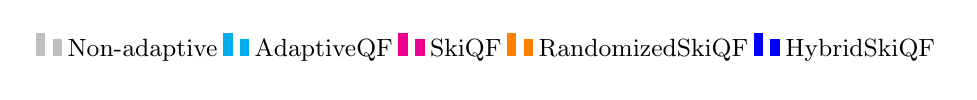
\begin{tikzpicture}
\begin{axis}[hide axis,xmin=0,xmax=1,ymin=0,ymax=1,
scale only axis,width=1cm,height=0.4cm,
legend columns=5,legend cell align=left,
legend style={draw=none,font=\small,at={(0.5,0.5)},anchor=center}]
\addlegendimage{ybar legend,/tikz/ybar,skiqfNonAdaptiveBar}
\addlegendentry{Non-adaptive}
\addlegendimage{ybar legend,/tikz/ybar,skiqfAdaptiveBar}
\addlegendentry{AdaptiveQF}
\addlegendimage{ybar legend,/tikz/ybar,skiqfSkiBar}
\addlegendentry{SkiQF}
\addlegendimage{ybar legend,/tikz/ybar,skiqfRandomizedBar}
\addlegendentry{RandomizedSkiQF}
\addlegendimage{ybar legend,/tikz/ybar,skiqfHybridBar}
\addlegendentry{HybridSkiQF}
\end{axis}\end{tikzpicture}
\par\medskip
\begingroup
\pgfmathsetlengthmacro{\skiqfpanelwidth}{(\linewidth-1.6cm-0.0cm)/1}
\begin{tikzpicture}\begin{groupplot}[skiqf axis,
group style={group size=1 by 1,horizontal sep=0.7cm,vertical sep=1.5cm},
scale only axis,width=\skiqfpanelwidth,height=3cm,scaled y ticks=true]
\nextgroupplot[title={Overall query throughput},
ylabel={Throughput\\(MOps/sec)},
ymin=0,
ybar=0,bar width=5pt,enlarge x limits=false,
xmin=-0.5,xmax=3.5,
xtick={0,1,2,3},
xticklabels={Uniform,Normal,Lognormal,Zipfian},
x tick label style={rotate=45,anchor=east,font=\scriptsize}]
\addplot[skiqfNonAdaptiveBar,mark size=1.8pt,mark repeat=1] coordinates {(0,1.817049) (1,1.858105) (2,1.843201) (3,4.148048)};
\addplot[skiqfAdaptiveBar,mark size=1.8pt,mark repeat=1] coordinates {(0,0.842753) (1,3.617783) (2,2.715952) (3,4.123663)};
\addplot[skiqfSkiBar,mark size=1.8pt,mark repeat=1] coordinates {(0,1.760643) (1,2.706858) (2,2.461892) (3,5.020314)};
\addplot[skiqfRandomizedBar,mark size=1.8pt,mark repeat=1] coordinates {(0,1.375574) (1,3.000158) (2,2.570689) (3,4.679129)};
\addplot[skiqfHybridBar,mark size=1.8pt,mark repeat=1] coordinates {(0,1.815552) (1,3.394378) (2,2.594401) (3,3.818818)};
\end{groupplot}\end{tikzpicture}\endgroup\end{center}

\begin{center}\small Final cumulative throughput; higher is better.\end{center}
\clearpage
\begin{center}
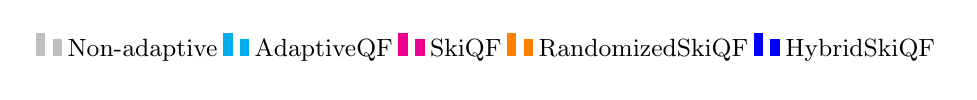
\begin{tikzpicture}
\begin{axis}[hide axis,xmin=0,xmax=1,ymin=0,ymax=1,
scale only axis,width=1cm,height=0.4cm,
legend columns=5,legend cell align=left,
legend style={draw=none,font=\small,at={(0.5,0.5)},anchor=center}]
\addlegendimage{ybar legend,/tikz/ybar,skiqfNonAdaptiveBar}
\addlegendentry{Non-adaptive}
\addlegendimage{ybar legend,/tikz/ybar,skiqfAdaptiveBar}
\addlegendentry{AdaptiveQF}
\addlegendimage{ybar legend,/tikz/ybar,skiqfSkiBar}
\addlegendentry{SkiQF}
\addlegendimage{ybar legend,/tikz/ybar,skiqfRandomizedBar}
\addlegendentry{RandomizedSkiQF}
\addlegendimage{ybar legend,/tikz/ybar,skiqfHybridBar}
\addlegendentry{HybridSkiQF}
\end{axis}\end{tikzpicture}
\par\medskip
\begingroup
\pgfmathsetlengthmacro{\skiqfpanelwidth}{(\linewidth-1.6cm-0.0cm)/1}
\begin{tikzpicture}\begin{groupplot}[skiqf axis,
group style={group size=1 by 1,horizontal sep=0.7cm,vertical sep=1.5cm},
scale only axis,width=\skiqfpanelwidth,height=3cm,scaled y ticks=true]
\nextgroupplot[title={Overall disk I/O},
ylabel={Bytes read\\(GiB)},
ymin=0,
ybar=0,bar width=5pt,enlarge x limits=false,
xmin=-0.5,xmax=3.5,
xtick={0,1,2,3},
xticklabels={Uniform,Normal,Lognormal,Zipfian},
x tick label style={rotate=45,anchor=east,font=\scriptsize}]
\addplot[skiqfNonAdaptiveBar,mark size=1.8pt,mark repeat=1] coordinates {(0,9.260845184) (1,9.016639709) (2,8.922481537) (3,3.481708527)};
\addplot[skiqfAdaptiveBar,mark size=1.8pt,mark repeat=1] coordinates {(0,15.41772079) (1,3.04441452) (2,4.428939819) (3,2.87959671)};
\addplot[skiqfSkiBar,mark size=1.8pt,mark repeat=1] coordinates {(0,8.962791443) (1,4.622535706) (2,5.509498596) (3,2.471111298)};
\addplot[skiqfRandomizedBar,mark size=1.8pt,mark repeat=1] coordinates {(0,11.10480499) (1,4.086284637) (2,5.151233673) (3,2.601951599)};
\addplot[skiqfHybridBar,mark size=1.8pt,mark repeat=1] coordinates {(0,8.957302094) (1,3.135982513) (2,4.507209778) (3,2.910675049)};
\end{groupplot}\end{tikzpicture}\endgroup\end{center}

\begin{center}\small Database plus reverse-map physical reads. Lower is better.\end{center}
\clearpage
\begin{center}
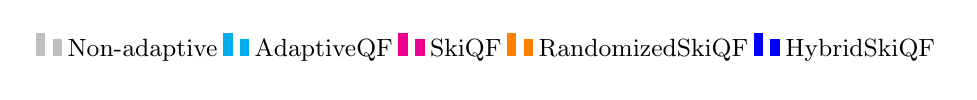
\begin{tikzpicture}
\begin{axis}[hide axis,xmin=0,xmax=1,ymin=0,ymax=1,
scale only axis,width=1cm,height=0.4cm,
legend columns=5,legend cell align=left,
legend style={draw=none,font=\small,at={(0.5,0.5)},anchor=center}]
\addlegendimage{ybar legend,/tikz/ybar,skiqfNonAdaptiveBar}
\addlegendentry{Non-adaptive}
\addlegendimage{ybar legend,/tikz/ybar,skiqfAdaptiveBar}
\addlegendentry{AdaptiveQF}
\addlegendimage{ybar legend,/tikz/ybar,skiqfSkiBar}
\addlegendentry{SkiQF}
\addlegendimage{ybar legend,/tikz/ybar,skiqfRandomizedBar}
\addlegendentry{RandomizedSkiQF}
\addlegendimage{ybar legend,/tikz/ybar,skiqfHybridBar}
\addlegendentry{HybridSkiQF}
\end{axis}\end{tikzpicture}
\par\medskip
\begingroup
\pgfmathsetlengthmacro{\skiqfpanelwidth}{(\linewidth-1.6cm-2.0999999999999996cm)/4}
\begin{tikzpicture}\begin{groupplot}[skiqf axis,
group style={group size=4 by 2,horizontal sep=0.7cm,vertical sep=1.5cm},
scale only axis,width=\skiqfpanelwidth,height=3cm,scaled y ticks=true]
\nextgroupplot[title={Uniform},
ylabel={Bytes read\\(GiB)},
ymin=0,
ybar=0,bar width=5pt,enlarge x limits=false,
xmin=-0.5,xmax=0.5,
xtick={0},
xticklabels={},
x tick label style={rotate=45,anchor=east,font=\scriptsize}]
\addplot[skiqfNonAdaptiveBar,mark size=1.8pt,mark repeat=1] coordinates {(0,9.260845184)};
\addplot[skiqfAdaptiveBar,mark size=1.8pt,mark repeat=1] coordinates {(0,8.943359375)};
\addplot[skiqfSkiBar,mark size=1.8pt,mark repeat=1] coordinates {(0,8.952911377)};
\addplot[skiqfRandomizedBar,mark size=1.8pt,mark repeat=1] coordinates {(0,8.946678162)};
\addplot[skiqfHybridBar,mark size=1.8pt,mark repeat=1] coordinates {(0,8.957214355)};
\nextgroupplot[title={Normal},
ymin=0,
ybar=0,bar width=5pt,enlarge x limits=false,
xmin=-0.5,xmax=0.5,
xtick={0},
xticklabels={},
x tick label style={rotate=45,anchor=east,font=\scriptsize}]
\addplot[skiqfNonAdaptiveBar,mark size=1.8pt,mark repeat=1] coordinates {(0,9.016639709)};
\addplot[skiqfAdaptiveBar,mark size=1.8pt,mark repeat=1] coordinates {(0,1.766857147)};
\addplot[skiqfSkiBar,mark size=1.8pt,mark repeat=1] coordinates {(0,3.401786804)};
\addplot[skiqfRandomizedBar,mark size=1.8pt,mark repeat=1] coordinates {(0,2.853275299)};
\addplot[skiqfHybridBar,mark size=1.8pt,mark repeat=1] coordinates {(0,1.855258942)};
\nextgroupplot[title={Lognormal},
ymin=0,
ybar=0,bar width=5pt,enlarge x limits=false,
xmin=-0.5,xmax=0.5,
xtick={0},
xticklabels={},
x tick label style={rotate=45,anchor=east,font=\scriptsize}]
\addplot[skiqfNonAdaptiveBar,mark size=1.8pt,mark repeat=1] coordinates {(0,8.922481537)};
\addplot[skiqfAdaptiveBar,mark size=1.8pt,mark repeat=1] coordinates {(0,2.573970795)};
\addplot[skiqfSkiBar,mark size=1.8pt,mark repeat=1] coordinates {(0,4.260837555)};
\addplot[skiqfRandomizedBar,mark size=1.8pt,mark repeat=1] coordinates {(0,3.696872711)};
\addplot[skiqfHybridBar,mark size=1.8pt,mark repeat=1] coordinates {(0,2.651622772)};
\nextgroupplot[title={Zipfian},
ymin=0,
ybar=0,bar width=5pt,enlarge x limits=false,
xmin=-0.5,xmax=0.5,
xtick={0},
xticklabels={},
x tick label style={rotate=45,anchor=east,font=\scriptsize}]
\addplot[skiqfNonAdaptiveBar,mark size=1.8pt,mark repeat=1] coordinates {(0,3.481708527)};
\addplot[skiqfAdaptiveBar,mark size=1.8pt,mark repeat=1] coordinates {(0,1.673542023)};
\addplot[skiqfSkiBar,mark size=1.8pt,mark repeat=1] coordinates {(0,2.12449646)};
\addplot[skiqfRandomizedBar,mark size=1.8pt,mark repeat=1] coordinates {(0,1.971427917)};
\addplot[skiqfHybridBar,mark size=1.8pt,mark repeat=1] coordinates {(0,1.696475983)};
\nextgroupplot[title={Uniform},
ylabel={False positives\\(millions)},
ymin=0,
ybar=0,bar width=5pt,enlarge x limits=false,
xmin=-0.5,xmax=0.5,
xtick={0},
xticklabels={},
x tick label style={rotate=45,anchor=east,font=\scriptsize}]
\addplot[skiqfNonAdaptiveBar,mark size=1.8pt,mark repeat=1] coordinates {(0,0.351454)};
\addplot[skiqfAdaptiveBar,mark size=1.8pt,mark repeat=1] coordinates {(0,0.350934)};
\addplot[skiqfSkiBar,mark size=1.8pt,mark repeat=1] coordinates {(0,0.351454)};
\addplot[skiqfRandomizedBar,mark size=1.8pt,mark repeat=1] coordinates {(0,0.351278)};
\addplot[skiqfHybridBar,mark size=1.8pt,mark repeat=1] coordinates {(0,0.351454)};
\nextgroupplot[title={Normal},
ymin=0,
ybar=0,bar width=5pt,enlarge x limits=false,
xmin=-0.5,xmax=0.5,
xtick={0},
xticklabels={},
x tick label style={rotate=45,anchor=east,font=\scriptsize}]
\addplot[skiqfNonAdaptiveBar,mark size=1.8pt,mark repeat=1] coordinates {(0,0.349015)};
\addplot[skiqfAdaptiveBar,mark size=1.8pt,mark repeat=1] coordinates {(0,0.069244)};
\addplot[skiqfSkiBar,mark size=1.8pt,mark repeat=1] coordinates {(0,0.135316)};
\addplot[skiqfRandomizedBar,mark size=1.8pt,mark repeat=1] coordinates {(0,0.113537)};
\addplot[skiqfHybridBar,mark size=1.8pt,mark repeat=1] coordinates {(0,0.072711)};
\nextgroupplot[title={Lognormal},
ymin=0,
ybar=0,bar width=5pt,enlarge x limits=false,
xmin=-0.5,xmax=0.5,
xtick={0},
xticklabels={},
x tick label style={rotate=45,anchor=east,font=\scriptsize}]
\addplot[skiqfNonAdaptiveBar,mark size=1.8pt,mark repeat=1] coordinates {(0,0.347868)};
\addplot[skiqfAdaptiveBar,mark size=1.8pt,mark repeat=1] coordinates {(0,0.100888)};
\addplot[skiqfSkiBar,mark size=1.8pt,mark repeat=1] coordinates {(0,0.168831)};
\addplot[skiqfRandomizedBar,mark size=1.8pt,mark repeat=1] coordinates {(0,0.146495)};
\addplot[skiqfHybridBar,mark size=1.8pt,mark repeat=1] coordinates {(0,0.104062)};
\nextgroupplot[title={Zipfian},
ymin=0,
ybar=0,bar width=5pt,enlarge x limits=false,
xmin=-0.5,xmax=0.5,
xtick={0},
xticklabels={},
x tick label style={rotate=45,anchor=east,font=\scriptsize}]
\addplot[skiqfNonAdaptiveBar,mark size=1.8pt,mark repeat=1] coordinates {(0,0.296627)};
\addplot[skiqfAdaptiveBar,mark size=1.8pt,mark repeat=1] coordinates {(0,0.065587)};
\addplot[skiqfSkiBar,mark size=1.8pt,mark repeat=1] coordinates {(0,0.084449)};
\addplot[skiqfRandomizedBar,mark size=1.8pt,mark repeat=1] coordinates {(0,0.078252)};
\addplot[skiqfHybridBar,mark size=1.8pt,mark repeat=1] coordinates {(0,0.067987)};
\end{groupplot}\end{tikzpicture}\endgroup\end{center}

\begin{center}\small Database I/O and false positives. Lower is better.\end{center}
\clearpage
\begin{center}
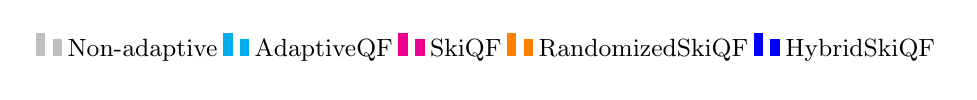
\begin{tikzpicture}
\begin{axis}[hide axis,xmin=0,xmax=1,ymin=0,ymax=1,
scale only axis,width=1cm,height=0.4cm,
legend columns=5,legend cell align=left,
legend style={draw=none,font=\small,at={(0.5,0.5)},anchor=center}]
\addlegendimage{ybar legend,/tikz/ybar,skiqfNonAdaptiveBar}
\addlegendentry{Non-adaptive}
\addlegendimage{ybar legend,/tikz/ybar,skiqfAdaptiveBar}
\addlegendentry{AdaptiveQF}
\addlegendimage{ybar legend,/tikz/ybar,skiqfSkiBar}
\addlegendentry{SkiQF}
\addlegendimage{ybar legend,/tikz/ybar,skiqfRandomizedBar}
\addlegendentry{RandomizedSkiQF}
\addlegendimage{ybar legend,/tikz/ybar,skiqfHybridBar}
\addlegendentry{HybridSkiQF}
\end{axis}\end{tikzpicture}
\par\medskip
\begingroup
\pgfmathsetlengthmacro{\skiqfpanelwidth}{(\linewidth-1.6cm-2.0999999999999996cm)/4}
\begin{tikzpicture}\begin{groupplot}[skiqf axis,
group style={group size=4 by 2,horizontal sep=0.7cm,vertical sep=1.5cm},
scale only axis,width=\skiqfpanelwidth,height=3cm,scaled y ticks=true]
\nextgroupplot[title={Uniform},
ylabel={Bytes read\\(GiB)},
ymin=0,
ybar=0,bar width=5pt,enlarge x limits=false,
xmin=-0.5,xmax=0.5,
xtick={0},
xticklabels={},
x tick label style={rotate=45,anchor=east,font=\scriptsize}]
\addplot[skiqfNonAdaptiveBar,mark size=1.8pt,mark repeat=1] coordinates {(0,0)};
\addplot[skiqfAdaptiveBar,mark size=1.8pt,mark repeat=1] coordinates {(0,6.47436142)};
\addplot[skiqfSkiBar,mark size=1.8pt,mark repeat=1] coordinates {(0,0.009880065918)};
\addplot[skiqfRandomizedBar,mark size=1.8pt,mark repeat=1] coordinates {(0,2.158126831)};
\addplot[skiqfHybridBar,mark size=1.8pt,mark repeat=1] coordinates {(0,8.773803711e-05)};
\nextgroupplot[title={Normal},
ymin=0,
ybar=0,bar width=5pt,enlarge x limits=false,
xmin=-0.5,xmax=0.5,
xtick={0},
xticklabels={},
x tick label style={rotate=45,anchor=east,font=\scriptsize}]
\addplot[skiqfNonAdaptiveBar,mark size=1.8pt,mark repeat=1] coordinates {(0,0)};
\addplot[skiqfAdaptiveBar,mark size=1.8pt,mark repeat=1] coordinates {(0,1.277557373)};
\addplot[skiqfSkiBar,mark size=1.8pt,mark repeat=1] coordinates {(0,1.220748901)};
\addplot[skiqfRandomizedBar,mark size=1.8pt,mark repeat=1] coordinates {(0,1.233009338)};
\addplot[skiqfHybridBar,mark size=1.8pt,mark repeat=1] coordinates {(0,1.280723572)};
\nextgroupplot[title={Lognormal},
ymin=0,
ybar=0,bar width=5pt,enlarge x limits=false,
xmin=-0.5,xmax=0.5,
xtick={0},
xticklabels={},
x tick label style={rotate=45,anchor=east,font=\scriptsize}]
\addplot[skiqfNonAdaptiveBar,mark size=1.8pt,mark repeat=1] coordinates {(0,0)};
\addplot[skiqfAdaptiveBar,mark size=1.8pt,mark repeat=1] coordinates {(0,1.854969025)};
\addplot[skiqfSkiBar,mark size=1.8pt,mark repeat=1] coordinates {(0,1.248661041)};
\addplot[skiqfRandomizedBar,mark size=1.8pt,mark repeat=1] coordinates {(0,1.454360962)};
\addplot[skiqfHybridBar,mark size=1.8pt,mark repeat=1] coordinates {(0,1.855587006)};
\nextgroupplot[title={Zipfian},
ymin=0,
ybar=0,bar width=5pt,enlarge x limits=false,
xmin=-0.5,xmax=0.5,
xtick={0},
xticklabels={},
x tick label style={rotate=45,anchor=east,font=\scriptsize}]
\addplot[skiqfNonAdaptiveBar,mark size=1.8pt,mark repeat=1] coordinates {(0,0)};
\addplot[skiqfAdaptiveBar,mark size=1.8pt,mark repeat=1] coordinates {(0,1.206054688)};
\addplot[skiqfSkiBar,mark size=1.8pt,mark repeat=1] coordinates {(0,0.3466148376)};
\addplot[skiqfRandomizedBar,mark size=1.8pt,mark repeat=1] coordinates {(0,0.6305236816)};
\addplot[skiqfHybridBar,mark size=1.8pt,mark repeat=1] coordinates {(0,1.214199066)};
\nextgroupplot[title={Uniform},
ylabel={Adaptations\\(millions)},
ymin=0,
ybar=0,bar width=5pt,enlarge x limits=false,
xmin=-0.5,xmax=0.5,
xtick={0},
xticklabels={},
x tick label style={rotate=45,anchor=east,font=\scriptsize}]
\addplot[skiqfNonAdaptiveBar,mark size=1.8pt,mark repeat=1] coordinates {(0,0)};
\addplot[skiqfAdaptiveBar,mark size=1.8pt,mark repeat=1] coordinates {(0,0.350934)};
\addplot[skiqfSkiBar,mark size=1.8pt,mark repeat=1] coordinates {(0,0.000523)};
\addplot[skiqfRandomizedBar,mark size=1.8pt,mark repeat=1] coordinates {(0,0.116972)};
\addplot[skiqfHybridBar,mark size=1.8pt,mark repeat=1] coordinates {(0,0)};
\nextgroupplot[title={Normal},
ymin=0,
ybar=0,bar width=5pt,enlarge x limits=false,
xmin=-0.5,xmax=0.5,
xtick={0},
xticklabels={},
x tick label style={rotate=45,anchor=east,font=\scriptsize}]
\addplot[skiqfNonAdaptiveBar,mark size=1.8pt,mark repeat=1] coordinates {(0,0)};
\addplot[skiqfAdaptiveBar,mark size=1.8pt,mark repeat=1] coordinates {(0,0.069244)};
\addplot[skiqfSkiBar,mark size=1.8pt,mark repeat=1] coordinates {(0,0.066087)};
\addplot[skiqfRandomizedBar,mark size=1.8pt,mark repeat=1] coordinates {(0,0.067147)};
\addplot[skiqfHybridBar,mark size=1.8pt,mark repeat=1] coordinates {(0,0.069211)};
\nextgroupplot[title={Lognormal},
ymin=0,
ybar=0,bar width=5pt,enlarge x limits=false,
xmin=-0.5,xmax=0.5,
xtick={0},
xticklabels={},
x tick label style={rotate=45,anchor=east,font=\scriptsize}]
\addplot[skiqfNonAdaptiveBar,mark size=1.8pt,mark repeat=1] coordinates {(0,0)};
\addplot[skiqfAdaptiveBar,mark size=1.8pt,mark repeat=1] coordinates {(0,0.100888)};
\addplot[skiqfSkiBar,mark size=1.8pt,mark repeat=1] coordinates {(0,0.067985)};
\addplot[skiqfRandomizedBar,mark size=1.8pt,mark repeat=1] coordinates {(0,0.078868)};
\addplot[skiqfHybridBar,mark size=1.8pt,mark repeat=1] coordinates {(0,0.100565)};
\nextgroupplot[title={Zipfian},
ymin=0,
ybar=0,bar width=5pt,enlarge x limits=false,
xmin=-0.5,xmax=0.5,
xtick={0},
xticklabels={},
x tick label style={rotate=45,anchor=east,font=\scriptsize}]
\addplot[skiqfNonAdaptiveBar,mark size=1.8pt,mark repeat=1] coordinates {(0,0)};
\addplot[skiqfAdaptiveBar,mark size=1.8pt,mark repeat=1] coordinates {(0,0.065587)};
\addplot[skiqfSkiBar,mark size=1.8pt,mark repeat=1] coordinates {(0,0.018874)};
\addplot[skiqfRandomizedBar,mark size=1.8pt,mark repeat=1] coordinates {(0,0.034238)};
\addplot[skiqfHybridBar,mark size=1.8pt,mark repeat=1] coordinates {(0,0.065138)};
\end{groupplot}\end{tikzpicture}\endgroup\end{center}

\begin{center}\small Reverse-map I/O and adaptations. Lower is better.\end{center}
\clearpage
\section{Adaptive adversary}
This new comparison extends the paper's adversarial study. Each filter receives its own feedback-dependent stream; each case identifies its feedback model.
\begin{center}
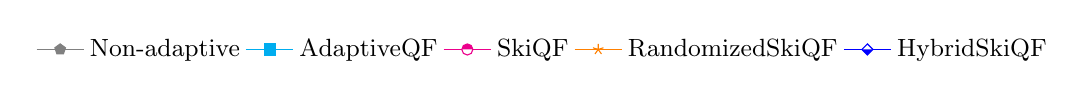
\begin{tikzpicture}
\begin{axis}[hide axis,xmin=0,xmax=1,ymin=0,ymax=1,
scale only axis,width=1cm,height=0.4cm,
legend columns=5,legend cell align=left,
legend style={draw=none,font=\small,at={(0.5,0.5)},anchor=center}]
\addlegendimage{skiqfNonAdaptive}
\addlegendentry{Non-adaptive}
\addlegendimage{skiqfAdaptive}
\addlegendentry{AdaptiveQF}
\addlegendimage{skiqfSki}
\addlegendentry{SkiQF}
\addlegendimage{skiqfRandomized}
\addlegendentry{RandomizedSkiQF}
\addlegendimage{skiqfHybrid}
\addlegendentry{HybridSkiQF}
\end{axis}\end{tikzpicture}
\par\medskip
\begingroup
\pgfmathsetlengthmacro{\skiqfpanelwidth}{(\linewidth-1.6cm-1.3cm)/2}
\begin{tikzpicture}\begin{groupplot}[skiqf axis,
group style={group size=2 by 1,horizontal sep=1.3cm,vertical sep=1.5cm},
scale only axis,width=\skiqfpanelwidth,height=3cm,scaled y ticks=true]
\nextgroupplot[title={Query throughput},
ylabel={Throughput\\(MOps/sec)},
ymin=0,
xlabel={Queries (millions)},
xmin=0,xmax=100,enlarge x limits=false]
\addplot[skiqfNonAdaptive,mark size=1.8pt,mark repeat=11] coordinates {(1,0.301487) (2,0.140198) (3,0.131647) (4,0.133119) (5,0.137779) (6,0.137238) (7,0.136589) (8,0.134375) (9,0.138181) (10,0.135279) (11,0.136083) (12,0.124457) (13,0.132323) (14,0.134081) (15,0.137774) (16,0.13452) (17,0.130437) (18,0.132451) (19,0.135369) (20,0.134375) (21,0.134768) (22,0.133785) (23,0.134112) (24,0.127984) (25,0.128786) (26,0.134703) (27,0.137972) (28,0.135877) (29,0.137156) (30,0.137433) (31,0.135637) (32,0.134132) (33,0.136871) (34,0.132734) (35,0.132963) (36,0.135713) (37,0.135544) (38,0.135516) (39,0.136033) (40,0.131334) (41,0.13851) (42,0.133205) (43,0.132292) (44,0.133655) (45,0.125768) (46,0.138912) (47,0.134029) (48,0.134081) (49,0.139119) (50,0.135881) (51,0.132161) (52,0.133826) (53,0.131116) (54,0.136993) (55,0.138129) (56,0.136226) (57,0.133108) (58,0.133797) (59,0.137238) (60,0.136223) (61,0.136728) (62,0.131777) (63,0.134309) (64,0.13722) (65,0.138312) (66,0.136344) (67,0.137953) (68,0.138238) (69,0.134964) (70,0.137734) (71,0.132822) (72,0.136287) (73,0.136768) (74,0.132189) (75,0.13553) (76,0.131047) (77,0.136696) (78,0.133574) (79,0.132527) (80,0.135224) (81,0.138304) (82,0.138243) (83,0.136066) (84,0.131935) (85,0.138557) (86,0.138241) (87,0.138164) (88,0.13583) (89,0.130863) (90,0.131339) (91,0.131647) (92,0.135863) (93,0.132488) (94,0.1354) (95,0.127961) (96,0.137081) (97,0.137888) (98,0.133118) (99,0.134101) (100,0.133247)};
\addplot[skiqfAdaptive,mark size=1.8pt,mark repeat=11] coordinates {(1,0.874312) (2,0.976421) (3,0.945378) (4,0.980449) (5,0.944162) (6,0.970258) (7,0.96623) (8,0.964589) (9,0.96891) (10,0.943447) (11,0.921965) (12,0.910805) (13,0.934554) (14,0.988902) (15,0.957261) (16,0.954862) (17,0.948911) (18,0.949411) (19,0.967148) (20,0.973051) (21,0.902198) (22,0.95047) (23,0.97932) (24,0.951279) (25,0.95336) (26,0.870671) (27,0.792493) (28,0.784896) (29,0.828862) (30,0.844554) (31,0.790916) (32,0.789477) (33,0.824804) (34,0.804618) (35,0.839183) (36,0.817752) (37,0.866766) (38,0.814071) (39,0.878279) (40,0.790221) (41,0.803531) (42,0.840701) (43,0.801273) (44,0.866605) (45,0.752898) (46,0.841902) (47,0.76615) (48,0.773631) (49,0.730488) (50,0.692972) (51,0.806432) (52,0.72703) (53,0.691203) (54,0.76476) (55,0.828147) (56,0.76366) (57,0.706347) (58,0.734185) (59,0.755641) (60,0.834116) (61,0.802308) (62,0.756202) (63,0.799945) (64,0.766653) (65,0.837248) (66,0.788663) (67,0.732776) (68,0.740148) (69,0.75484) (70,0.766973) (71,0.814823) (72,0.724931) (73,0.743712) (74,0.842904) (75,0.741988) (76,0.742357) (77,0.833079) (78,0.750048) (79,0.891057) (80,0.791482) (81,0.780803) (82,0.71686) (83,0.794319) (84,0.778661) (85,0.810778) (86,0.744194) (87,0.849714) (88,0.85064) (89,0.893479) (90,0.836417) (91,0.850416) (92,0.80888) (93,0.858861) (94,0.777835) (95,0.823783) (96,0.804927) (97,0.931765) (98,0.847766) (99,0.83718) (100,0.765605)};
\addplot[skiqfSki,mark size=1.8pt,mark repeat=11] coordinates {(1,0.801329) (2,0.769473) (3,0.758558) (4,0.848153) (5,0.653426) (6,0.678868) (7,0.643008) (8,0.650013) (9,0.648656) (10,0.631588) (11,0.640651) (12,0.571608) (13,0.642594) (14,0.641339) (15,0.635723) (16,0.628848) (17,0.61442) (18,0.6536) (19,0.652085) (20,0.653243) (21,0.645781) (22,0.651589) (23,0.66836) (24,0.612999) (25,0.622841) (26,0.624194) (27,0.624217) (28,0.662549) (29,0.677333) (30,0.619356) (31,0.664219) (32,0.648079) (33,0.609599) (34,0.619136) (35,0.6248) (36,0.625703) (37,0.648008) (38,0.642499) (39,0.641705) (40,0.636648) (41,0.640881) (42,0.63166) (43,0.647371) (44,0.634264) (45,0.633204) (46,0.622836) (47,0.62107) (48,0.631705) (49,0.63784) (50,0.630825) (51,0.637069) (52,0.662266) (53,0.613951) (54,0.645918) (55,0.662393) (56,0.608572) (57,0.600178) (58,0.666257) (59,0.609474) (60,0.669982) (61,0.633126) (62,0.657997) (63,0.604837) (64,0.626044) (65,0.575411) (66,0.625996) (67,0.639807) (68,0.578892) (69,0.645059) (70,0.661058) (71,0.657973) (72,0.66285) (73,0.643654) (74,0.672491) (75,0.663054) (76,0.653087) (77,0.662108) (78,0.668634) (79,0.649566) (80,0.650206) (81,0.655738) (82,0.645784) (83,0.629626) (84,0.670408) (85,0.679049) (86,0.664273) (87,0.664984) (88,0.671597) (89,0.677027) (90,0.691019) (91,0.667528) (92,0.659764) (93,0.673545) (94,0.663301) (95,0.669055) (96,0.657009) (97,0.675136) (98,0.675714) (99,0.668376) (100,0.663858)};
\addplot[skiqfRandomized,mark size=1.8pt,mark repeat=11] coordinates {(1,0.880858) (2,0.797258) (3,0.776646) (4,0.793399) (5,0.798936) (6,0.813466) (7,0.923685) (8,0.887188) (9,0.710367) (10,0.698004) (11,0.715112) (12,0.705464) (13,0.70688) (14,0.716018) (15,0.692483) (16,0.697666) (17,0.675607) (18,0.725494) (19,0.699067) (20,0.744344) (21,0.711134) (22,0.668608) (23,0.687345) (24,0.662191) (25,0.688205) (26,0.698649) (27,0.667181) (28,0.705839) (29,0.717349) (30,0.705541) (31,0.69496) (32,0.720301) (33,0.674904) (34,0.690218) (35,0.681959) (36,0.680145) (37,0.725839) (38,0.726202) (39,0.715379) (40,0.724077) (41,0.647201) (42,0.719796) (43,0.676866) (44,0.688154) (45,0.668756) (46,0.717197) (47,0.708187) (48,0.652926) (49,0.698847) (50,0.69263) (51,0.708768) (52,0.723467) (53,0.684274) (54,0.716926) (55,0.722742) (56,0.69659) (57,0.733497) (58,0.773244) (59,0.745113) (60,0.762907) (61,0.739695) (62,0.748264) (63,0.7534) (64,0.777858) (65,0.733077) (66,0.741527) (67,0.755936) (68,0.728281) (69,0.739674) (70,0.727509) (71,0.747362) (72,0.755318) (73,0.733235) (74,0.728634) (75,0.724249) (76,0.732248) (77,0.761278) (78,0.767465) (79,0.726174) (80,0.725473) (81,0.731781) (82,0.730228) (83,0.72345) (84,0.757025) (85,0.766768) (86,0.728132) (87,0.759671) (88,0.7594) (89,0.763438) (90,0.756379) (91,0.73607) (92,0.746658) (93,0.71735) (94,0.739101) (95,0.755762) (96,0.742498) (97,0.744444) (98,0.754469) (99,0.748555) (100,0.75075)};
\addplot[skiqfHybrid,mark size=1.8pt,mark repeat=11] coordinates {(1,0.281083) (2,0.906047) (3,0.920857) (4,0.831937) (5,0.843607) (6,0.870087) (7,0.912221) (8,0.86399) (9,0.901172) (10,0.872046) (11,0.899014) (12,0.136865) (13,0.840035) (14,0.930242) (15,0.842449) (16,0.861439) (17,0.904101) (18,0.857917) (19,0.917675) (20,0.970768) (21,0.137638) (22,0.943898) (23,0.968742) (24,0.955875) (25,0.949254) (26,0.953956) (27,0.928918) (28,0.949755) (29,0.985712) (30,0.132339) (31,0.942844) (32,0.905753) (33,0.798283) (34,0.889889) (35,0.874811) (36,0.871855) (37,0.896855) (38,0.901118) (39,0.140658) (40,0.821344) (41,0.917682) (42,0.900208) (43,0.868468) (44,0.855737) (45,0.897149) (46,0.883015) (47,0.813417) (48,0.139984) (49,0.870875) (50,0.884276) (51,0.883772) (52,0.846555) (53,0.870116) (54,0.844592) (55,0.960711) (56,0.879297) (57,0.137353) (58,0.837005) (59,0.86687) (60,0.911209) (61,0.913417) (62,0.89076) (63,0.90608) (64,0.905145) (65,0.139706) (66,0.909748) (67,0.93688) (68,0.913194) (69,0.947299) (70,0.919773) (71,0.923363) (72,0.94577) (73,0.135057) (74,0.913674) (75,0.953048) (76,0.940883) (77,0.959702) (78,0.924108) (79,0.937128) (80,0.923303) (81,0.137827) (82,0.949337) (83,0.890865) (84,0.932559) (85,0.956871) (86,0.949761) (87,0.942715) (88,0.952642) (89,0.961226) (90,0.137339) (91,0.934776) (92,0.934717) (93,0.942124) (94,0.910093) (95,0.961079) (96,0.93758) (97,0.932864) (98,0.947684) (99,0.138311) (100,0.950706)};
\nextgroupplot[title={False positives},
ylabel={False positive rate},
ymin=0,
xlabel={Queries (millions)},
xmin=0,xmax=100,enlarge x limits=false]
\addplot[skiqfNonAdaptive,mark size=1.8pt,mark repeat=11] coordinates {(1,0.053302) (2,0.053365) (3,0.053359) (4,0.053317) (5,0.053353) (6,0.053379) (7,0.053281) (8,0.053309) (9,0.053273) (10,0.053377) (11,0.053417) (12,0.053329) (13,0.053409) (14,0.053324) (15,0.053216) (16,0.053374) (17,0.053314) (18,0.053408) (19,0.053344) (20,0.053338) (21,0.053279) (22,0.053272) (23,0.053384) (24,0.053304) (25,0.053327) (26,0.053366) (27,0.053347) (28,0.053379) (29,0.05336) (30,0.053285) (31,0.05325) (32,0.053346) (33,0.053332) (34,0.053328) (35,0.053327) (36,0.053364) (37,0.053417) (38,0.053361) (39,0.053347) (40,0.05332) (41,0.053325) (42,0.053317) (43,0.053365) (44,0.053338) (45,0.053332) (46,0.053215) (47,0.053339) (48,0.053393) (49,0.053312) (50,0.053339) (51,0.053334) (52,0.053327) (53,0.053359) (54,0.053284) (55,0.053323) (56,0.053395) (57,0.05325) (58,0.053281) (59,0.053461) (60,0.053437) (61,0.053255) (62,0.053389) (63,0.053238) (64,0.053365) (65,0.053382) (66,0.053304) (67,0.053258) (68,0.053357) (69,0.053429) (70,0.05332) (71,0.053432) (72,0.053376) (73,0.053369) (74,0.053372) (75,0.053302) (76,0.053398) (77,0.053401) (78,0.053337) (79,0.053341) (80,0.053403) (81,0.053249) (82,0.053309) (83,0.053343) (84,0.053367) (85,0.053398) (86,0.0533) (87,0.05351) (88,0.053316) (89,0.053308) (90,0.053313) (91,0.053371) (92,0.053339) (93,0.053281) (94,0.053255) (95,0.053344) (96,0.053363) (97,0.053387) (98,0.053282) (99,0.0534) (100,0.053263)};
\addplot[skiqfAdaptive,mark size=1.8pt,mark repeat=11] coordinates {(1,0.003494) (2,0.003507) (3,0.003553) (4,0.003499) (5,0.003523) (6,0.003525) (7,0.003486) (8,0.003471) (9,0.003496) (10,0.003568) (11,0.003481) (12,0.003622) (13,0.003526) (14,0.00342) (15,0.00351) (16,0.003491) (17,0.00357) (18,0.003526) (19,0.003512) (20,0.003433) (21,0.003487) (22,0.003541) (23,0.003467) (24,0.003501) (25,0.003555) (26,0.00351) (27,0.003566) (28,0.003514) (29,0.003395) (30,0.003545) (31,0.003427) (32,0.003524) (33,0.00351) (34,0.003549) (35,0.003575) (36,0.003543) (37,0.003504) (38,0.003493) (39,0.003499) (40,0.003529) (41,0.003475) (42,0.003557) (43,0.003479) (44,0.003374) (45,0.003527) (46,0.003589) (47,0.003475) (48,0.003493) (49,0.003466) (50,0.0035) (51,0.003507) (52,0.003451) (53,0.003587) (54,0.00344) (55,0.003425) (56,0.003628) (57,0.003625) (58,0.00341) (59,0.003593) (60,0.003387) (61,0.003556) (62,0.003517) (63,0.003488) (64,0.003412) (65,0.00356) (66,0.003569) (67,0.003524) (68,0.003633) (69,0.003557) (70,0.003463) (71,0.00354) (72,0.00353) (73,0.003578) (74,0.003526) (75,0.00347) (76,0.003587) (77,0.003393) (78,0.003495) (79,0.003495) (80,0.003573) (81,0.003512) (82,0.003525) (83,0.003639) (84,0.003444) (85,0.003503) (86,0.003515) (87,0.003531) (88,0.003459) (89,0.003436) (90,0.003478) (91,0.003492) (92,0.003581) (93,0.003452) (94,0.00356) (95,0.003437) (96,0.00348) (97,0.003485) (98,0.003495) (99,0.003504) (100,0.003505)};
\addplot[skiqfSki,mark size=1.8pt,mark repeat=11] coordinates {(1,0.006857) (2,0.006895) (3,0.006942) (4,0.006835) (5,0.006902) (6,0.006916) (7,0.006858) (8,0.00682) (9,0.006833) (10,0.007005) (11,0.006841) (12,0.007077) (13,0.006937) (14,0.006714) (15,0.006825) (16,0.006834) (17,0.007036) (18,0.006831) (19,0.006949) (20,0.006734) (21,0.006829) (22,0.006926) (23,0.006794) (24,0.006879) (25,0.006886) (26,0.006957) (27,0.006971) (28,0.006885) (29,0.006675) (30,0.006935) (31,0.006773) (32,0.006841) (33,0.006874) (34,0.006981) (35,0.006967) (36,0.006957) (37,0.00694) (38,0.0068) (39,0.006836) (40,0.00684) (41,0.006887) (42,0.006879) (43,0.006858) (44,0.006635) (45,0.006956) (46,0.006957) (47,0.006854) (48,0.006879) (49,0.006812) (50,0.006904) (51,0.006762) (52,0.006746) (53,0.007093) (54,0.006814) (55,0.006642) (56,0.00707) (57,0.007145) (58,0.006749) (59,0.006971) (60,0.006656) (61,0.006974) (62,0.00695) (63,0.006795) (64,0.006746) (65,0.006992) (66,0.00695) (67,0.006862) (68,0.007163) (69,0.00693) (70,0.006838) (71,0.006932) (72,0.006873) (73,0.007064) (74,0.006952) (75,0.006787) (76,0.006986) (77,0.006753) (78,0.006733) (79,0.006864) (80,0.006996) (81,0.00703) (82,0.006786) (83,0.007196) (84,0.006854) (85,0.006729) (86,0.006923) (87,0.006871) (88,0.00691) (89,0.006724) (90,0.006692) (91,0.00693) (92,0.006989) (93,0.006888) (94,0.006916) (95,0.006749) (96,0.006828) (97,0.006791) (98,0.006857) (99,0.00687) (100,0.0069)};
\addplot[skiqfRandomized,mark size=1.8pt,mark repeat=11] coordinates {(1,0.005739) (2,0.00585) (3,0.005894) (4,0.005771) (5,0.005825) (6,0.005809) (7,0.005772) (8,0.005666) (9,0.005726) (10,0.005854) (11,0.005692) (12,0.005925) (13,0.005803) (14,0.005665) (15,0.005734) (16,0.005714) (17,0.005915) (18,0.005767) (19,0.005766) (20,0.005683) (21,0.005707) (22,0.005774) (23,0.005661) (24,0.005754) (25,0.005801) (26,0.005821) (27,0.005851) (28,0.005777) (29,0.005607) (30,0.005827) (31,0.005684) (32,0.005637) (33,0.005801) (34,0.005844) (35,0.005846) (36,0.005813) (37,0.005779) (38,0.005684) (39,0.005717) (40,0.005747) (41,0.005843) (42,0.005775) (43,0.005705) (44,0.00557) (45,0.005855) (46,0.005883) (47,0.005677) (48,0.005759) (49,0.005744) (50,0.005747) (51,0.005719) (52,0.005652) (53,0.005898) (54,0.005686) (55,0.005594) (56,0.005906) (57,0.005928) (58,0.005604) (59,0.005814) (60,0.005637) (61,0.005769) (62,0.005782) (63,0.005746) (64,0.005545) (65,0.005934) (66,0.005825) (67,0.005709) (68,0.006016) (69,0.005816) (70,0.005725) (71,0.005813) (72,0.005732) (73,0.005925) (74,0.005809) (75,0.005738) (76,0.005851) (77,0.005591) (78,0.00564) (79,0.005773) (80,0.005854) (81,0.005799) (82,0.005694) (83,0.005921) (84,0.005707) (85,0.005632) (86,0.005824) (87,0.005739) (88,0.005748) (89,0.005653) (90,0.00566) (91,0.005825) (92,0.005804) (93,0.005771) (94,0.005832) (95,0.005663) (96,0.00572) (97,0.005705) (98,0.005691) (99,0.005778) (100,0.00577)};
\addplot[skiqfHybrid,mark size=1.8pt,mark repeat=11] coordinates {(1,0.053302) (2,0.003513) (3,0.003562) (4,0.003496) (5,0.003517) (6,0.003543) (7,0.003487) (8,0.003469) (9,0.003493) (10,0.003562) (11,0.003482) (12,0.053397) (13,0.003584) (14,0.003419) (15,0.003476) (16,0.003477) (17,0.003607) (18,0.003504) (19,0.003518) (20,0.003438) (21,0.053249) (22,0.003556) (23,0.003486) (24,0.0035) (25,0.003528) (26,0.003526) (27,0.003562) (28,0.003516) (29,0.003394) (30,0.053351) (31,0.003452) (32,0.003516) (33,0.003519) (34,0.003564) (35,0.003515) (36,0.003571) (37,0.003548) (38,0.003474) (39,0.05329) (40,0.00353) (41,0.003523) (42,0.003471) (43,0.003505) (44,0.003403) (45,0.003496) (46,0.003561) (47,0.003531) (48,0.053246) (49,0.003459) (50,0.003526) (51,0.003506) (52,0.003397) (53,0.003586) (54,0.003548) (55,0.003335) (56,0.003585) (57,0.053462) (58,0.003457) (59,0.003598) (60,0.003392) (61,0.003507) (62,0.003538) (63,0.003495) (64,0.00342) (65,0.053325) (66,0.003612) (67,0.003485) (68,0.003644) (69,0.003505) (70,0.003539) (71,0.003554) (72,0.003491) (73,0.053354) (74,0.003598) (75,0.003445) (76,0.003527) (77,0.003453) (78,0.003473) (79,0.003452) (80,0.003534) (81,0.053427) (82,0.003522) (83,0.003618) (84,0.003493) (85,0.003485) (86,0.003482) (87,0.003538) (88,0.003497) (89,0.003451) (90,0.053227) (91,0.003542) (92,0.003537) (93,0.003522) (94,0.003552) (95,0.003437) (96,0.003462) (97,0.003516) (98,0.003468) (99,0.053315) (100,0.003516)};
\end{groupplot}\end{tikzpicture}\endgroup\end{center}

\begin{center}\small Perfect recognition of ordinary query outcomes: corrections immediately disable replay; tolerated false positives enable it. There are no probes or adversary windows. HybridSkiQF's detector window is 1,000,000 negative-key queries; smoothing remains 0.7 and the repeated-FP threshold remains 6.\end{center}
\begin{center}
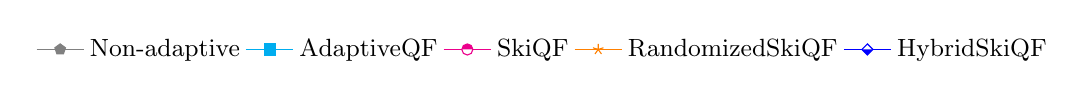
\begin{tikzpicture}
\begin{axis}[hide axis,xmin=0,xmax=1,ymin=0,ymax=1,
scale only axis,width=1cm,height=0.4cm,
legend columns=5,legend cell align=left,
legend style={draw=none,font=\small,at={(0.5,0.5)},anchor=center}]
\addlegendimage{skiqfNonAdaptive}
\addlegendentry{Non-adaptive}
\addlegendimage{skiqfAdaptive}
\addlegendentry{AdaptiveQF}
\addlegendimage{skiqfSki}
\addlegendentry{SkiQF}
\addlegendimage{skiqfRandomized}
\addlegendentry{RandomizedSkiQF}
\addlegendimage{skiqfHybrid}
\addlegendentry{HybridSkiQF}
\end{axis}\end{tikzpicture}
\par\medskip
\begingroup
\pgfmathsetlengthmacro{\skiqfpanelwidth}{(\linewidth-1.6cm-0.0cm)/1}
\begin{tikzpicture}\begin{groupplot}[skiqf axis,
group style={group size=1 by 1,horizontal sep=0.7cm,vertical sep=1.5cm},
scale only axis,width=\skiqfpanelwidth,height=3cm,scaled y ticks=true]
\nextgroupplot[title={Replay flag},
ylabel={Fraction of queries\\with replay enabled},
ymin=0,
xlabel={Queries (millions)},
xmin=0,xmax=100,enlarge x limits=false]
\addplot[skiqfNonAdaptive,mark size=1.8pt,mark repeat=11] coordinates {(1,0.999851) (2,1) (3,1) (4,1) (5,1) (6,1) (7,1) (8,1) (9,1) (10,1) (11,1) (12,1) (13,1) (14,1) (15,1) (16,1) (17,1) (18,1) (19,1) (20,1) (21,1) (22,1) (23,1) (24,1) (25,1) (26,1) (27,1) (28,1) (29,1) (30,1) (31,1) (32,1) (33,1) (34,1) (35,1) (36,1) (37,1) (38,1) (39,1) (40,1) (41,1) (42,1) (43,1) (44,1) (45,1) (46,1) (47,1) (48,1) (49,1) (50,1) (51,1) (52,1) (53,1) (54,1) (55,1) (56,1) (57,1) (58,1) (59,1) (60,1) (61,1) (62,1) (63,1) (64,1) (65,1) (66,1) (67,1) (68,1) (69,1) (70,1) (71,1) (72,1) (73,1) (74,1) (75,1) (76,1) (77,1) (78,1) (79,1) (80,1) (81,1) (82,1) (83,1) (84,1) (85,1) (86,1) (87,1) (88,1) (89,1) (90,1) (91,1) (92,1) (93,1) (94,1) (95,1) (96,1) (97,1) (98,1) (99,1) (100,1)};
\addplot[skiqfAdaptive,mark size=1.8pt,mark repeat=11] coordinates {(1,0) (2,0) (3,0) (4,0) (5,0) (6,0) (7,0) (8,0) (9,0) (10,0) (11,0) (12,0) (13,0) (14,0) (15,0) (16,0) (17,0) (18,0) (19,0) (20,0) (21,0) (22,0) (23,0) (24,0) (25,0) (26,0) (27,0) (28,0) (29,0) (30,0) (31,0) (32,0) (33,0) (34,0) (35,0) (36,0) (37,0) (38,0) (39,0) (40,0) (41,0) (42,0) (43,0) (44,0) (45,0) (46,0) (47,0) (48,0) (49,0) (50,0) (51,0) (52,0) (53,0) (54,0) (55,0) (56,0) (57,0) (58,0) (59,0) (60,0) (61,0) (62,0) (63,0) (64,0) (65,0) (66,0) (67,0) (68,0) (69,0) (70,0) (71,0) (72,0) (73,0) (74,0) (75,0) (76,0) (77,0) (78,0) (79,0) (80,0) (81,0) (82,0) (83,0) (84,0) (85,0) (86,0) (87,0) (88,0) (89,0) (90,0) (91,0) (92,0) (93,0) (94,0) (95,0) (96,0) (97,0) (98,0) (99,0) (100,0)};
\addplot[skiqfSki,mark size=1.8pt,mark repeat=11] coordinates {(1,0.035825) (2,0.035496) (3,0.035709) (4,0.035981) (5,0.036224) (6,0.036085) (7,0.036045) (8,0.03557) (9,0.03529) (10,0.03611) (11,0.035641) (12,0.036813) (13,0.036153) (14,0.03482) (15,0.035306) (16,0.0355) (17,0.036455) (18,0.035461) (19,0.036156) (20,0.035119) (21,0.035555) (22,0.035607) (23,0.035596) (24,0.036078) (25,0.03532) (26,0.036401) (27,0.036562) (28,0.036055) (29,0.034484) (30,0.035392) (31,0.034711) (32,0.035972) (33,0.035136) (34,0.036488) (35,0.036278) (36,0.036074) (37,0.036752) (38,0.035568) (39,0.035905) (40,0.036683) (41,0.035633) (42,0.03566) (43,0.035574) (44,0.034894) (45,0.036086) (46,0.035782) (47,0.035707) (48,0.035543) (49,0.035022) (50,0.035922) (51,0.03579) (52,0.034745) (53,0.037541) (54,0.036138) (55,0.03413) (56,0.037031) (57,0.037343) (58,0.034554) (59,0.036731) (60,0.034493) (61,0.036196) (62,0.036023) (63,0.03555) (64,0.035398) (65,0.036567) (66,0.035981) (67,0.03595) (68,0.037823) (69,0.036012) (70,0.035736) (71,0.036378) (72,0.036084) (73,0.03686) (74,0.035899) (75,0.035466) (76,0.036528) (77,0.035429) (78,0.034845) (79,0.035705) (80,0.036464) (81,0.036194) (82,0.03555) (83,0.037083) (84,0.035382) (85,0.034953) (86,0.036398) (87,0.036109) (88,0.036116) (89,0.034818) (90,0.034674) (91,0.035854) (92,0.036225) (93,0.03586) (94,0.035918) (95,0.035158) (96,0.035305) (97,0.035367) (98,0.035674) (99,0.035643) (100,0.035747)};
\addplot[skiqfRandomized,mark size=1.8pt,mark repeat=11] coordinates {(1,0.023653) (2,0.02473) (3,0.025205) (4,0.024356) (5,0.024583) (6,0.024283) (7,0.023995) (8,0.023335) (9,0.023505) (10,0.02455) (11,0.023585) (12,0.024274) (13,0.024522) (14,0.023819) (15,0.024156) (16,0.023656) (17,0.02501) (18,0.024544) (19,0.023516) (20,0.023579) (21,0.023746) (22,0.023637) (23,0.023051) (24,0.024042) (25,0.024622) (26,0.024277) (27,0.024381) (28,0.024301) (29,0.023788) (30,0.023949) (31,0.023782) (32,0.022953) (33,0.024576) (34,0.023886) (35,0.024419) (36,0.02382) (37,0.024372) (38,0.023791) (39,0.02367) (40,0.023453) (41,0.024644) (42,0.023901) (43,0.023904) (44,0.023548) (45,0.024123) (46,0.023823) (47,0.02347) (48,0.02371) (49,0.024464) (50,0.024165) (51,0.024244) (52,0.024239) (53,0.023938) (54,0.023523) (55,0.02324) (56,0.024149) (57,0.023989) (58,0.022577) (59,0.023692) (60,0.023423) (61,0.024134) (62,0.023735) (63,0.023906) (64,0.023303) (65,0.024523) (66,0.024274) (67,0.023818) (68,0.025387) (69,0.02382) (70,0.02373) (71,0.024005) (72,0.023835) (73,0.024687) (74,0.024335) (75,0.023866) (76,0.023741) (77,0.022698) (78,0.023631) (79,0.024386) (80,0.025186) (81,0.024185) (82,0.023199) (83,0.024194) (84,0.024151) (85,0.023575) (86,0.024013) (87,0.023301) (88,0.023739) (89,0.023037) (90,0.023567) (91,0.02493) (92,0.02405) (93,0.024156) (94,0.024298) (95,0.023304) (96,0.023733) (97,0.02405) (98,0.0235) (99,0.024742) (100,0.024304)};
\addplot[skiqfHybrid,mark size=1.8pt,mark repeat=11] coordinates {(1,0.999851) (2,1e-06) (3,0) (4,0) (5,0) (6,0) (7,0) (8,0) (9,0) (10,0) (11,0) (12,0.999639) (13,1e-06) (14,0) (15,0) (16,0) (17,0) (18,0) (19,0) (20,0) (21,0.999311) (22,1e-06) (23,0) (24,0) (25,0) (26,0) (27,0) (28,0) (29,0) (30,0.999771) (31,1e-06) (32,0) (33,0) (34,0) (35,0) (36,0) (37,0) (38,0) (39,0.999763) (40,1e-06) (41,0) (42,0) (43,0) (44,0) (45,0) (46,0) (47,0) (48,0.998478) (49,1e-06) (50,0) (51,0) (52,0) (53,0) (54,0) (55,0) (56,0) (57,0.999862) (58,1e-06) (59,0) (60,0) (61,0) (62,0) (63,0) (64,0) (65,0.999596) (66,1e-06) (67,0) (68,0) (69,0) (70,0) (71,0) (72,0) (73,0.999437) (74,1e-06) (75,0) (76,0) (77,0) (78,0) (79,0) (80,0) (81,0.999936) (82,1e-06) (83,0) (84,0) (85,0) (86,0) (87,0) (88,0) (89,0) (90,0.999977) (91,1e-06) (92,0) (93,0) (94,0) (95,0) (96,0) (97,0) (98,0) (99,0.999859) (100,1e-06)};
\end{groupplot}\end{tikzpicture}\endgroup\end{center}

\begin{center}\small The flag changes immediately; the plot averages its value over each reporting interval.\end{center}
\begin{center}
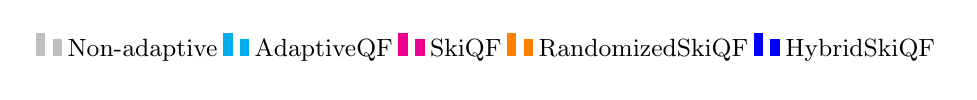
\begin{tikzpicture}
\begin{axis}[hide axis,xmin=0,xmax=1,ymin=0,ymax=1,
scale only axis,width=1cm,height=0.4cm,
legend columns=5,legend cell align=left,
legend style={draw=none,font=\small,at={(0.5,0.5)},anchor=center}]
\addlegendimage{ybar legend,/tikz/ybar,skiqfNonAdaptiveBar}
\addlegendentry{Non-adaptive}
\addlegendimage{ybar legend,/tikz/ybar,skiqfAdaptiveBar}
\addlegendentry{AdaptiveQF}
\addlegendimage{ybar legend,/tikz/ybar,skiqfSkiBar}
\addlegendentry{SkiQF}
\addlegendimage{ybar legend,/tikz/ybar,skiqfRandomizedBar}
\addlegendentry{RandomizedSkiQF}
\addlegendimage{ybar legend,/tikz/ybar,skiqfHybridBar}
\addlegendentry{HybridSkiQF}
\end{axis}\end{tikzpicture}
\par\medskip
\begingroup
\pgfmathsetlengthmacro{\skiqfpanelwidth}{(\linewidth-1.6cm-0.0cm)/1}
\begin{tikzpicture}\begin{groupplot}[skiqf axis,
group style={group size=1 by 1,horizontal sep=0.7cm,vertical sep=1.5cm},
scale only axis,width=\skiqfpanelwidth,height=3cm,scaled y ticks=true]
\nextgroupplot[title={Corrections by traffic regime},
ylabel={Corrections},
ymin=0,
ybar=0,bar width=5pt,enlarge x limits=false,
xmin=-0.5,xmax=1.5,
xtick={0,1},
xticklabels={Replay disabled,Replay enabled},
x tick label style={rotate=45,anchor=east,font=\scriptsize}]
\addplot[skiqfNonAdaptiveBar,mark size=1.8pt,mark repeat=1] coordinates {(0,0) (1,0)};
\addplot[skiqfAdaptiveBar,mark size=1.8pt,mark repeat=1] coordinates {(0,350934) (1,0)};
\addplot[skiqfSkiBar,mark size=1.8pt,mark repeat=1] coordinates {(0,20) (1,338247)};
\addplot[skiqfRandomizedBar,mark size=1.8pt,mark repeat=1] coordinates {(0,113864) (1,228634)};
\addplot[skiqfHybridBar,mark size=1.8pt,mark repeat=1] coordinates {(0,308681) (1,12)};
\end{groupplot}\end{tikzpicture}\endgroup\end{center}

\begin{center}\small Regimes refer to the flag before the query; a correction disables replay for the next query.\end{center}
\begin{center}
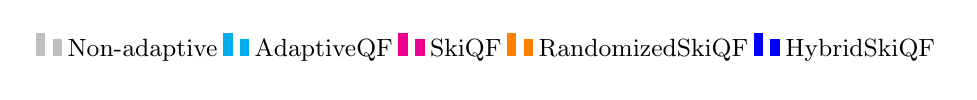
\begin{tikzpicture}
\begin{axis}[hide axis,xmin=0,xmax=1,ymin=0,ymax=1,
scale only axis,width=1cm,height=0.4cm,
legend columns=5,legend cell align=left,
legend style={draw=none,font=\small,at={(0.5,0.5)},anchor=center}]
\addlegendimage{ybar legend,/tikz/ybar,skiqfNonAdaptiveBar}
\addlegendentry{Non-adaptive}
\addlegendimage{ybar legend,/tikz/ybar,skiqfAdaptiveBar}
\addlegendentry{AdaptiveQF}
\addlegendimage{ybar legend,/tikz/ybar,skiqfSkiBar}
\addlegendentry{SkiQF}
\addlegendimage{ybar legend,/tikz/ybar,skiqfRandomizedBar}
\addlegendentry{RandomizedSkiQF}
\addlegendimage{ybar legend,/tikz/ybar,skiqfHybridBar}
\addlegendentry{HybridSkiQF}
\end{axis}\end{tikzpicture}
\par\medskip
\begingroup
\pgfmathsetlengthmacro{\skiqfpanelwidth}{(\linewidth-1.6cm-1.3cm)/2}
\begin{tikzpicture}\begin{groupplot}[skiqf axis,
group style={group size=2 by 1,horizontal sep=1.3cm,vertical sep=1.5cm},
scale only axis,width=\skiqfpanelwidth,height=3cm,scaled y ticks=true]
\nextgroupplot[title={Overall throughput},
ylabel={Throughput\\(MOps/sec)},
ymin=0,
ybar=0,bar width=5pt,enlarge x limits=false,
xmin=-0.5,xmax=0.5,
xtick={0},
xticklabels={Immediate feedback},
x tick label style={rotate=45,anchor=east,font=\scriptsize}]
\addplot[skiqfNonAdaptiveBar,mark size=1.8pt,mark repeat=1] coordinates {(0,0.135454)};
\addplot[skiqfAdaptiveBar,mark size=1.8pt,mark repeat=1] coordinates {(0,0.82827)};
\addplot[skiqfSkiBar,mark size=1.8pt,mark repeat=1] coordinates {(0,0.648501)};
\addplot[skiqfRandomizedBar,mark size=1.8pt,mark repeat=1] coordinates {(0,0.727537)};
\addplot[skiqfHybridBar,mark size=1.8pt,mark repeat=1] coordinates {(0,0.553586)};
\nextgroupplot[title={Overall FPR},
ylabel={False positive rate},
ymin=0,
ybar=0,bar width=5pt,enlarge x limits=false,
xmin=-0.5,xmax=0.5,
xtick={0},
xticklabels={Immediate feedback},
x tick label style={rotate=45,anchor=east,font=\scriptsize}]
\addplot[skiqfNonAdaptiveBar,mark size=1.8pt,mark repeat=1] coordinates {(0,0.05333935)};
\addplot[skiqfAdaptiveBar,mark size=1.8pt,mark repeat=1] coordinates {(0,0.00350934)};
\addplot[skiqfSkiBar,mark size=1.8pt,mark repeat=1] coordinates {(0,0.00688029)};
\addplot[skiqfRandomizedBar,mark size=1.8pt,mark repeat=1] coordinates {(0,0.00576227)};
\addplot[skiqfHybridBar,mark size=1.8pt,mark repeat=1] coordinates {(0,0.00948638)};
\end{groupplot}\end{tikzpicture}\endgroup\end{center}

\begin{center}\small Final cumulative measurements. Throughput: higher is better; FPR: lower is better.\end{center}
}{Medium validation and execution are pending. No large experiment has started.}

\begin{thebibliography}{9}
\bibitem{karlin} A. R. Karlin, M. S. Manasse, L. A. McGeoch, and S. Owicki, \emph{Competitive Randomized Algorithms for Non-Uniform Problems}, SODA 1990, pp. 301--309, especially Theorem 1, p. 303. \url{https://courses.csail.mit.edu/6.895/fall03/handouts/papers/karlin.pdf}.
\bibitem{background} A. M\k{a}dry and D. Panigrahi, \emph{The Semi-stochastic Ski-rental Problem}, introduction and discussion of the classical model. \url{https://madry.mit.edu/docs/skirental.pdf}.
\end{thebibliography}
\end{document}
